\documentclass[oneside, a4paper, 11pt]{book}
\usepackage{titlesec}
% \usepackage[utf8]{inputenc}
\usepackage{graphicx}
% \usepackage{subfiles}
\usepackage{fancyhdr}
\usepackage[top=2cm, bottom=2cm, bmargin=2cm]{geometry}
% \usepackage[nottoc, numbib]{tocbibind}
\usepackage{listings}
\usepackage{color}
\usepackage{caption}
\usepackage{float}
\usepackage[caption = false]{subfig}
% \usepackage{subcaption}
\usepackage{amsmath}
\usepackage{hyperref}

% Just to get the page numbering right
\pagestyle{fancy}
\fancyhf{}
\renewcommand{\headrulewidth}{0pt}
\cfoot{\thepage}

% paths to the same images folder relative to the root and the "sections" folders.
\graphicspath{{images/}{../images/}}

\title{\Huge \textbf{Modelling of\\Gene Regulatory Networks using Microarray Data}\\Work Report}
\author{Shivam Rana}

\titleformat{\chapter}
  {\Large\bfseries} % format
  {}                % label
  {0pt}             % sep
  {\huge}

\titlespacing{\chapter}{0pc}{0.8pc}{0.8pc}

\definecolor{codegreen}{rgb}{0,0.6,0}
\definecolor{codegray}{rgb}{0.5,0.5,0.5}
\definecolor{codepurple}{rgb}{0.58,0,0.82}

\lstdefinestyle{mystyle}{
    backgroundcolor=\color{white},   
    commentstyle=\color{codegreen},
    keywordstyle=\color{magenta},
    numberstyle=\tiny\color{codegray},
    stringstyle=\color{codepurple},
    basicstyle=\footnotesize,
    breakatwhitespace=false,         
    breaklines=true,                 
    frame=single,
    captionpos=b,                    
    keepspaces=true,                 
    numbers=left,                    
    numbersep=5pt,                  
    showspaces=false,                
    showstringspaces=false,
    showtabs=false,                  
    tabsize=2
}
 
\lstset{style=mystyle}

\begin{document}

\frontmatter
\date{}
\maketitle

\tableofcontents
\mainmatter


%%%%%%%%%%%%%%%%%%%%%%%%%%%%%%
%%%%%% ACKNOWLEDGEMENTS %%%%%%
%%%%%%%%%%%%%%%%%%%%%%%%%%%%%%
\chapter*{Acknowledgements}
I would like to thank \href{https://www.iiitd.edu.in/~vikram/}{Prof. Vikram Goyal} and \href{https://www.iiitd.ac.in/sriram}{Prof. K. Sriram} for guiding me throughout the duration of the internship.
I would also like to thank National Network for Mathematics and Computational Biology for giving me this opportunity to work on this research project.
\medskip
\medskip

Shivam Rana


%%%%%%%%%%%%%%%%%%%%%%%
%%%%%% OBJECTIVE %%%%%%
%%%%%%%%%%%%%%%%%%%%%%%
\chapter{Objective}
\markboth{}{}
A Gene Regulatory Network is a collection of regulators that interact with each other and with other substances in the cell to govern the gene expression levels of messenger ribonucleic acid and proteins. Expressions of different genes may have a positive or negative effects on the others. Microarray Data or Gene Expression Data represents the expression level of various genes under certain experimental conditions. Our objective is to model the GRNs using the microarray data.


%%%%%%%%%%%%%%%%%%%%%%
%%%%% MOTIVATION %%%%%
%%%%%%%%%%%%%%%%%%%%%%
\chapter{Motivation}
\markboth{}{}
\section{So, why Gene Regulatory Networks?}
Gene regulatory networks (GRNs) have an important role in every process of life, including cell differentiation, metabolism, the cell cycle and signal transduction. It is important to emphasize that the inference of gene regulatory networks is not the final result, but these networks are supposed to help in solving a number of different biological and biomedical problems. Some problems GRNs can help solve, discussed in the following sections, might give you an idea of how GRNs can be helpful.

\section{Causal map of molecular interactions}
The most common use of the GRNs might be to serve as a \textit{map} or a \textit{blueprint} of molecular interactions. Thus, such a network can be used to derive a biological hypothesis about molecular interactions (eg., for the transcription regulation of genes), which can then be investigated in wet lab experiments. In such a case, GRNs represent causal biochemical interactions because the predicted links are supposed to correspond to actual physical binding events between molecules. An important aspect of this application is that the GRNs represent statistically significant predictions of molecular interactions obtained from large-scale data. Given the very large number of potential interactions between ~20,000 genes in Human and ~6000 gene in yeast, the GRNs are of tremendous help in narrowing these numbers down to potential interactions for which statistical support is available. Overall, this enables more effective experiments by an adopted experimental design.

\section{Comparative network analysis}
When more and more gene regulatory networks from different physiological and disease conditions become available, it will be possible to statistically compare these networks. This will allow to learn about interaction changes across different physiological or disease conditions and enrich our biological and biomedical understanding of such phenotypes. It might be challenging to determine which similarity or distance measures are suitable to perform such a comparative network analysis and different types of networks as well as different biological questions may require different approaches.

However, in order for this approach to succeed it will be necessary to establish databases, similar to sequence or protein structure databases, that provide free access to the inferred gene regulatory networks from different physiological and disease conditions.

\section{Network medicine and drug design}
For establishing a network medicine useful for clinicians, it will be necessary to integrate different types of gene networks with each other, because each network type carries information about particular molecular aspects. For example, whereas the transcriptional regulatory network contains only information about the controlling regulations of gene expression, protein interaction networks represent information about protein-protein complexes. Taken together, an integration of various important molecular interaction types results in a comprehensive overview of regulatory programs and organizational architectures. Also, information about temporal (time varying) changes in the network structure are important to understand immune response, infection and differentiation processes.

Also, for a more efficient design of rational drugs the utilization of gene networks are indispensable. This would allow to create, e.g., a connectivity map that is based on the similarity of molecular interaction networks rather than on the mere similarity of expression profiles. Overall, this would help us on our way to a more personalized medicine, because condition specific gene regulatory networks are closer to the phenotype\footnote{\textbf{Phenotype} is an organism's actual observed properties, such as morphology, development, or behavior. This distinction is fundamental in the study of inheritance of traits and their evolution.} than genetic\footnote{\textbf{Genetics} is the study of genes, heredity, and genetic variation in living organisms.} or epigenetic\footnote{\textbf{Epigenetics} is the study, in the field of genetics, of cellular and physiological phenotypic trait variations that are caused by external or environmental factors that switch genes on and off and affect how cells read genes instead of being caused by changes in the DNA sequence.} markers.


%%%%%%%%%%%%%%%%%%%%%%
%%%% INTRODUCTION %%%%
%%%%%%%%%%%%%%%%%%%%%%
\chapter{Introduction}
\markboth{}{}
\section{What is a GRN?}
The genes, regulators, and the regulatory connections between them, together with an interpretation scheme form gene network. \textbf{Regulators} are proteins, RNAs and other metabolites which can regulate (encourage or inhibit the expression levels) the genes. In general, each \textbf{mRNA (Messenger Ribonucleic acid)} molecule makes a protein (or set of proteins). Some proteins serve only to activate other genes, and these are called the \textbf{transcription factors} (regulators), the main players in regulatory networks. Each gene has a region called \textbf{cis-region} (promoter region), where the regulator binds and turns them on, initiating the production of another protein, and so on\cite{streib}.

A GRN represents the functionally related genes, that is, genes which are causally linked and not just correlated. GRN models can span from genetic interaction maps to physical interaction graphs to models of network dynamics and gene expression kinetics. \medskip

\begin{figure}[h]
    \centering
    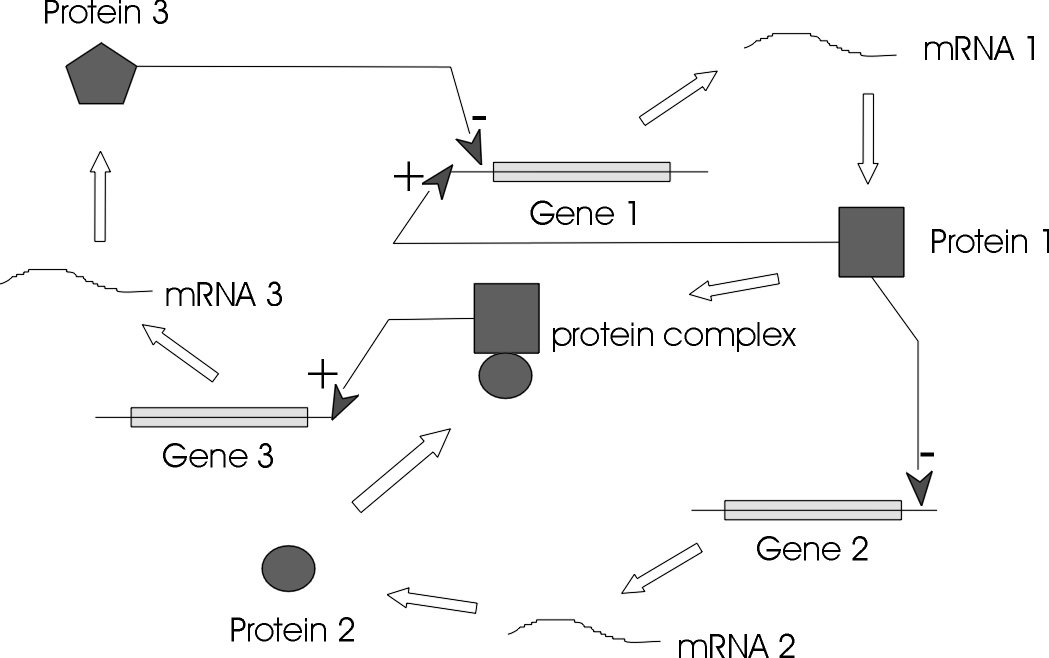
\includegraphics[scale=0.70]{regulation.JPG}
    \caption {\texttt{A Genetic Regulatory Network}}
    \captionsetup{singlelinecheck=off,font=footnotesize, width=0.8\textwidth}
    \caption*{Gene 1 produces mRNA 1 which produces the Protein 1. Now, Protein 1 binds on \textit{cis-region} of Gene 2 and inhibits it. Gene 2 in turn produces Protein 2 through mRNA 2, which binds to the another Protein to make a protein complex. Now, this protein complex binds to Gene 3 and promotes it to produce mRNA 3 which makes the Protein 3. Finally, Protein 1 and Protein 3 binds to the Gene 1 and promotes and inhibits it, respectively. This, completes the cycle. Thus, here we have 2 feedback loops. Note that it is not necessary that there will only be feedback loops in a GRN. This example just shows a very small part of a GRN. A GRN usually consists of thousands of genes.}
\end{figure}

\section{What is microarray data?}
Microarray Data or Gene Expression Data represents gene expression of genes in a particular tissue of the body under certain experimental conditions. A DNA microarray (also commonly known as DNA chip or biochip) is a collection of microscopic DNA spots attached to a solid surface. Scientists use DNA microarrays to measure the expression levels of large numbers of genes simultaneously or to genotype multiple regions of a genome. Each DNA spot contains picomoles of a specific DNA sequence, known as probes (or reporters or oligos). These can be a short section of a gene or other DNA element that are used to hybridize a cDNA or cRNA (also called anti-sense RNA) sample (called target) under high-stringency conditions. Probe-target hybridization is usually detected and quantified by detection of fluorophore, silver, or chemiluminescence-labeled targets to determine relative abundance of nucleic acid sequences in the target. Microarray data can be used to model the GRNs. So, for the analysis part we have a decimal values for each gene for each experiment.

\begin{figure}[h]
    \centering
    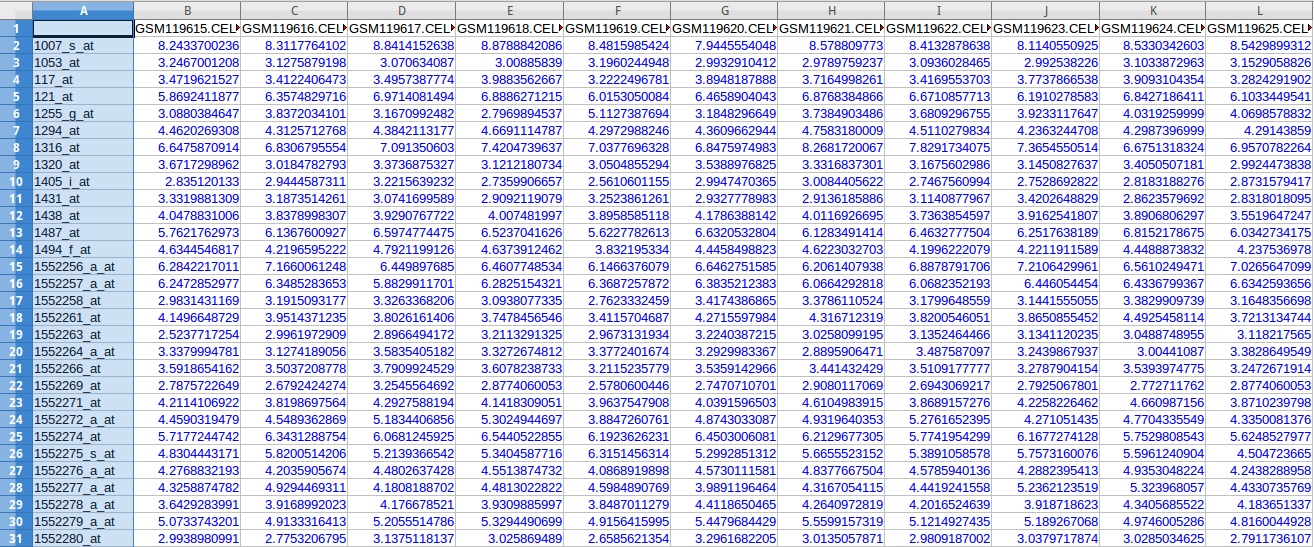
\includegraphics[width=\textwidth]{microarray.png}
    \caption {\texttt{A Sample Microarray Data}}
    \captionsetup{singlelinecheck=off,font=footnotesize, width=0.8\textwidth}
    \caption*{The selected column is the gene column. Each string ending with "\_at" is a gene. Other columns represent experiments with each decimal value pertaining to the expression value of that gene in that particular experiment. There are 150 other columns (experiments) that couldn't be shown in the snapshot.}
\end{figure}

\section{Different methods for modelling GRNs}
There are a variety of modeling techniques\cite{bolouri} that can be used for representing GRNs. Some are summarised below.

\subsection{Graph Theoretical Models}
Graph Theoretical Models (GTM) mainly describe the topology/architecture of a gene network. They describe the feature relationship between genes and possibly their nature. GTMs are particularly useful for knowledge representation. 

Gene networks are represented by graph structure, G(V,E), where V ($V = \{1, 2, 3, \ldots,\\ n\}$) represents the gene regulatory elements (genes, proteins) and E ($E = \{(i, j)|i,j \in V\}$) represents interactions between them (activation, inhibition, causality, binding specificity). The edges can be directed (indicating that one node is the precursor to other) or weighted (indicating the strength). The nodes and edges both can be labelled with function or nature of the relationship (activator, activation, inhibitor, inhibition, etc).

GTMs are not particularly useful as they can't show the dynamics of the network. One can't perform simulations on the gene networks using GTMS.

\subsection{Bayesian Networks}
A Bayesian network is basically an annotated directed acyclic graph G(X, E), where the nodes represent random variables (or gene expressions) and the edges indicate the conditional dependencies between the nodes (genes). Each node is associated with a probability function that takes, as input, a particular set of values for the node's parent variables, and gives (as output) the probability (or probability distribution, if applicable) of the variable represented by the node. The technique is based on the the assumption that given a node's parents, each variable is independent of its non-descendants. Thus, each Bayesian network uniquely specifies a decomposition of the joint distribution over all variables down to the conditional distributions of the nodes\cite{heckerman, zou}. The figure \ref{bayes} will explain the Bayesian network using an example although the example does not belong to the Biology domain.

\begin{figure}[h]
    \centering
    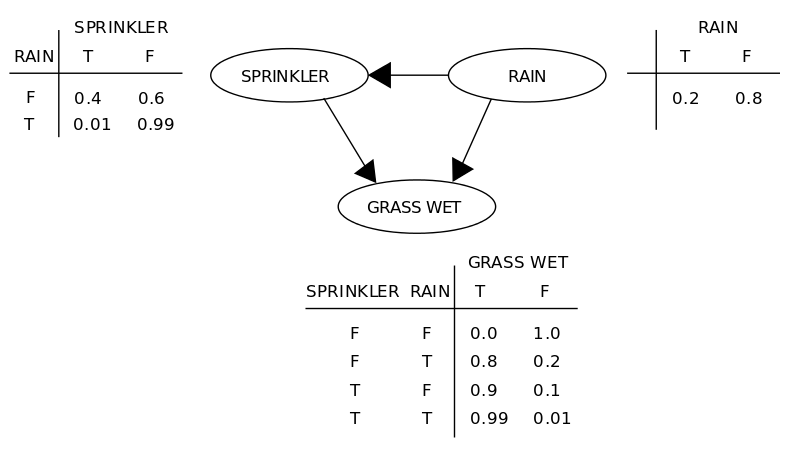
\includegraphics[width=\textwidth]{bn.png}
    \caption {\texttt{A simple Bayesian network}}
    \captionsetup{singlelinecheck=off,font=footnotesize, width=0.8\textwidth}
    \caption*{Assuming there are two events which could cause grass to be wet: either the sprinkler is on or it's raining. Also, suppose that the rain has a direct effect on the use of the sprinkler (namely that when it rains, the sprinkler is usually not turned on). Then the situation can be modeled with a Bayesian network (shown). All three variables have two possible values, T (for true) and F (for false). [Figure taken from wikipedia.]}
\end{figure}

\subsection{Boolean Networks}
A Boolean network is a directed graph $G(X, E)$, where the nodes are boolean variables with an associated boolean function. Each gene is represented by a node and state of each node is determined by the boolean function. Assuming an ideal situation, each node has two states - on or off (1 or 0). At any given time, the states (values) of all nodes represent the state of the network. All states’ transitions together correspond to a state transition of the network from $S(t)$ to the new network state, $S(t + 1)$. Synchronicity is another assumption of the boolean networks. Thus, whole network transits from state $S(t)$ to state $S(t+1)$. A series of state transitions is called a trajectory\cite{vladmir}.

\begin{figure}[h]
    \centering
    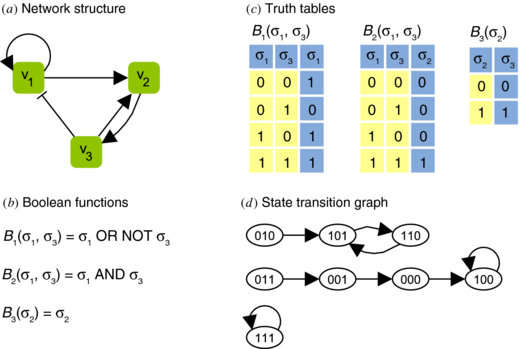
\includegraphics[width=\textwidth]{BN2.jpg}
    \caption {\texttt{A made up Boolean network}}
    \label{bayes}
\end{figure}

\section{Pre-processing} \label{preprocess}
Data-gathering methods are often loosely controlled, resulting in out-of-range values, impossible data combinations, missing values, etc. Analyzing data that has not been carefully screened for such problems can produce misleading results. Thus, the representation and quality of data is first and foremost before running an analysis. It includes cleaning, normalization, transformation, feature extraction and selection, etc.

\subsection{Pre-processing in this study}
\begin{itemize}
  \item Normalization
  \item Quality Control
  \item Filtering and differential expression
\end{itemize}

\textbf{Quality Control} (QC) assessment is a crucial first step in successful data analysis: before any comparisons can be performed it is necessary to check that there were no problems with sample processing, and that arrays are of sufficient quality to be included in a study.
\newline

\textbf{Normalization} is a broad term for methods that are used for removing systematic variations from DNA microarray data. In other words, normalization makes the measurements from different arrays inter-comparable. The methods are largely dissimilar for different DNA microarray technologies. Robust multiarray average (RMA) is a commonly used method for preprocessing and normalizing microarray data.
\newline

\textbf{Filtering}, is to exclude some part of the data. There are two kinds - unspecific and specific filtering. \textbf{Unspecific filtering} refers to methods for excluding a certain part of the data without any knowledge of the grouping of the samples. It is typically used for excluding any uninteresting genes from the dataset. Genes that are not changing at all during the experiment or are expressed on a very low level so that their measurements are unreliable, are usually excluded from further analyses. \textbf{Specific filtering} is used is situations when the filtering is affected by the known grouping of the samples. For example, in a case-control study genes that are expressed on a very low level across all samples might be removed in an unspecific filtering process. Genes could also be removed from the data using some statistical test or some other method that requires group knowledge.

If the filtering in truly unspecific, then no bias has been introduced to the statistical testing, and it’s results should be valid. If in doubt whether to filter or not, one can always first run a statistical test, and after that use unspecific filtering.

\section{Statistical Analyses}
Statistical analysis of DNA microarray experiments is still under heavy development. There are no consensus, no strict guidelines or real rules of thumb when to apply some tests and when never to apply certain other tests. One of the widely used tools for the statistical analysis is \texttt{limma}, which implements
linear models. One of the assumptions of the limma’s method is that the data is normally distributed (otherwise the significance tests give wrong results), but the real world data is not always normally distributed. From a typical Affymetrix experiment, maybe only about 20\% of the expression values are normally distributed (inferred from several chips, of course). Other are non-normally distributed, and one should probably use non-parametric methods for the analysis. However, usually the same method is used for all genes, and the results are therefore only approximate. One can probably rank the genes according to the p-values, but assuming that the p-values are unbiased in the traditional statistical sense is an illusion.

\subsection{Design matrix (or model matrix)}
The design matrix contains data on the \textit{independent variables} (also called explanatory variables) in statistical models (e.g., the general linear model) which attempt to explain observed data on a \textit{response variable} (often called a \textit{dependent variable}) in terms of the explanatory variables. It can contain indicator variables (ones and zeros) that indicate group membership in an ANOVA\footnote{\textbf{Analysis of variance (ANOVA)} is a collection of statistical models used to analyze the differences among group means and their associated procedures (such as "variation" among and between groups), developed by statistician and evolutionary biologist Ronald Fisher.}, or it can contain values of continuous variables.
\newline

In a regression model, written in matrix-vector form as

$$y=X\beta+ \epsilon$$

the matrix $X$ is the design matrix, while $y$ is the vector of observations on the dependent variable, $\beta$ is a vector of response coefficients (one for each explanatory variable) and $\epsilon$ is a vector containing the values of the model's error term for the various observations. In the design matrix, each column is a vector of observations on one of the explanatory variables.
\newline

\subsection{One-way ANOVA \protect{(offset from reference group)}}
In our case, the ANOVA model could be equivalently written as each group parameter $\tau_i$ being an offset from some overall reference. Typically, this reference point is taken to be one of the groups under consideration. This makes sense in the context of comparing multiple treatment groups to a control group and the control group is considered the \textit{reference}. In the following example, group 1 was chosen to be the reference group. As such the model to be fit is

$$y_{ij} = \mu + \tau_i + \epsilon_{ij}$$

with the constraint that $\tau_1$ is zero.

$$
\begin{bmatrix}
    y_1 \\ y_2 \\ y_3 \\ y_4 \\ y_5 \\ y_6 \\ y_7
\end{bmatrix} = 
\begin{bmatrix}
    1 &0 &0 \\1 &0  &0 \\ 1 & 0 & 0 \\ 1 & 1 & 0 \\ 1 & 1 & 0 \\ 1 & 0 & 1 \\ 1  & 0 & 1
\end{bmatrix}
\begin{bmatrix}
    \mu \\  \tau_2 \\ \tau_3
\end{bmatrix} +
\begin{bmatrix} 
    \epsilon_1 \\ \epsilon_2 \\ \epsilon_3 \\ \epsilon_4 \\ \epsilon_5 \\ \epsilon_6 \\ \epsilon_7
\end{bmatrix}
$$

In this model $\mu$ is the mean of the reference group and $\tau_i$ is the difference from group i to the reference group. $\tau_1$ is not included in the matrix because its difference from the reference group (itself) is necessarily zero.

\subsection{Analyses using linear model}
The method to be used is called \textbf{empirical Bayes}\footnote{\textbf{Empirical Bayes methods} are procedures for statistical inference in which the prior distribution is estimated from the data. Empirical Bayes may be viewed as an approximation to a fully Bayesian treatment of a hierarchical model wherein the parameters at the highest level of the hierarchy are set to their most likely values, instead of being integrated out.}, since it uses a method where certain parameter are inferred from the data (hence, empirical), and Bayes is term used to describe certain approaches in statistics.

Empirical Bayes is a better analysis method than, traditional \textbf{t-test}\footnote{A \textbf{t-test} is any statistical hypothesis test in which the test statistic follows a Student's t-distribution if the null hypothesis is supported.} for DNA microarray data, since it gives us more precise estimates of the statistical significance of the genes.

\section{Gene Set Enrichment Analysis (GSEA)}
GSEA is used to describe all methods that are used for statistically testing whether genes in our list of interesting genes are enriched in some pathways or functional categories. Typically these methods employ \textit{hypergeometric test based statistics}\footnote{In probability theory and statistics, the \textbf{hypergeometric distribution} is a discrete probability distribution that describes the probability of k successes in n draws, without replacement, from a finite population of size N that contains exactly K successes, wherein each draw is either a success or a failure. In contrast, the binomial distribution describes the probability of k successes in n draws with replacement. In statistics, the \textbf{hypergeometric test} uses the hypergeometric distribution to calculate the statistical significance of having drawn a specific k successes (out of n total draws) from the aforementioned population. The test is often used to identify which sub-populations are over- or under-represented in a sample.}. Prior to this a statistical test is typically conducted in order to find the statistically significantly regulated genes from the data.

\subsection{GO categories}
Gene ontology (GO) is a major bioinformatics initiative to unify the representation of gene and gene product attributes across all species. More specifically, the project aims to: 

\begin{enumerate}
    \item Maintain and develop its controlled vocabulary of gene and gene product attributes.
    \item Annotate genes and gene products, and assimilate and disseminate annotation data.
    \item Provide tools for easy access to all aspects of the data provided by the project, and to enable functional interpretation of experimental data using the GO, for example via enrichment analysis.
\end{enumerate}

An ontology is a representation of something we know about. "Ontologies" consist of a representation of things that are detectable or directly observable, and the relationships between those things. The ontology covers three domains:

\begin{itemize}
    \item \textbf{Cellular component}, the parts of a cell or its extracellular environment
    \item \textbf{Molecular function}, the elemental activities of a gene product at the molecular level, such as binding or catalysis
    \item \textbf{Biological process}, operations or sets of molecular events with a defined beginning and end, pertinent to the functioning of integrated living units: cells, tissues, organs, and organisms.
\end{itemize}

Each GO term within the ontology has a term name, which may be a word or string of words; a unique alphanumeric identifier; a definition with cited sources; and a namespace indicating the domain to which it belongs. The GO ontology is structured as a directed acyclic graph, and each term has defined relationships to one or more other terms in the same domain, and sometimes to other domains. The GO vocabulary is designed to be species-neutral, and includes terms applicable to prokaryotes and eukaryotes, single and multicellular organisms. The GO ontology file is freely available from the GO website\footnote{http://amigo.geneontology.org/}.

\subsection{KEGG pathways}
KEGG (Kyoto Encyclopedia of Genes and Genomes) is a collection of databases dealing with genomes, biological pathways, diseases, drugs, and chemical substances. The KEGG database project was initiated in 1995 by Minoru Kanehisa, Professor at the Institute for Chemical Research, Kyoto University, under the then ongoing Japanese Human Genome Program.

It is a collection of manually drawn KEGG pathway maps representing experimental knowledge on metabolism and various other functions of the cell and the organism. Each pathway map contains a network of molecular interactions and reactions and is designed to link genes in the genome to gene products (mostly proteins) in the pathway. This has enabled the analysis called KEGG pathway mapping, whereby the gene content in the genome is compared with the KEGG PATHWAY database to examine which pathways and associated functions are likely to be encoded in the genome.

\section{Clustering}
\subsection{Heatmap or Hierarchical Clustering}
Heatmap presents hierarchical clustering of both genes and arrays, and additionally displays the expression patterns, all in the same visualization.

\subsubsection{Clusterig}
In order to decide where a cluster should be split (for divisive), a measure of dissimilarity between sets of observations is required. In most methods of hierarchical clustering, this is achieved by use of an appropriate metric (a measure of distance between pairs of observations), and a linkage criterion which specifies the dissimilarity of sets as a function of the pairwise distances of observations in the sets. Following two phases make up the clustering process,

\begin{itemize}
  \item Calculation of pairwise distances
  \item Selection of tree construction method or linkage criteria
\end{itemize}

\medskip
\textbf{Calculation of pairwise distances} between genes and between samples (arrays) are calculated using a selected distance measure. The choice of an appropriate metric will influence the shape of the clusters, as some elements may be close to one another according to one distance and farther away according to another. For example, in a 2-dimensional space, the distance between the point (1,0) and the origin (0,0) is always 1 according to the usual norms, but the distance between the point (1,1) and the origin (0,0) can be 2 under Manhattan distance, $\scriptstyle\sqrt{2}$ under Euclidean distance. Some commonly used distance metrics are - euclidean distance\footnote{$d = \sqrt{\sum_i (a_i-b_i)^2}$} or pearson correlation\footnote{$d = 1-r$ where $r = \frac{Z(x) . Z(y)}{n}$, or in other words, dot-product of the z-scores of the vectors x and y. The z-score of x is constructed by subtracting from x its mean and dividing by its standard deviation.}.

\medskip
\textbf{Linkage criteria} determines the distance between sets of observations as a function of the pairwise distances between observations. In other words, this parameter specifies how the distance between clusters is measured. Some commonly used  linkage criteria between two sets of observations A and B and a chosen metric d, are - Maximum or complete-linkage clustering\footnote{$\max \, \{\, d(a,b) : a \in A,\, b \in B \,\}$}, Minimum or single-linkage clustering\footnote{$\min \, \{\, d(a,b) : a \in A,\, b \in B \,\}$}, Mean or average linkage clustering, or UPGMA\footnote{$\frac{1}{|A| |B|} \sum_{a \in A }\sum_{ b \in B} d(a,b)$}.

\subsubsection{Color Schemes}
There are many different color schemes that can be used to illustrate the heatmap, with perceptual advantages and disadvantages for each. Rainbow colormaps are often used, as humans can perceive more shades of color than they can of gray, and this would purportedly increase the amount of detail perceivable in the image. However, this is discouraged by many in the scientific community. The usual coloring scheme for microarray data in heatmaps is to present down-regulated genes with green, and up-regulated genes with red. You'll see an example of a heatmap in the next chapter.

\subsection{k-Means Clustering}
k-means clustering aims to partition n observations into k clusters in which each observation belongs to the cluster with the nearest mean, serving as a prototype of the cluster. The problem is computationally difficult (NP-hard); however, there are efficient heuristic algorithms that are commonly employed and converge quickly to a local optimum. 

k-means clustering does not produce a tree, but divides the genes or arrays into a number of clusters. In contrast to hierarchical clustering, k-means clustering is feasible even for very large datasets. Before the analysis, user has to specify how many clusters should be returned. Unfortunately, there are no good rules of thumb for estimating the starting number of clusters before the analysis. Although, a technique will be discussed in next chapter which gives us a good estimate for the number of clusters.

\subsubsection{Standard algorithm\protect\footnote{The following description of the algorithm has been taken from the Wikipedia article}}
The most common algorithm uses an iterative refinement technique.
Given an initial set of k means $m_1(1)$, \ldots, $m_k(1)$, the algorithm proceeds by alternating between two steps:

\textbf{Assignment step}: Assign each observation to the cluster whose mean yields the least within-cluster sum of squares (WCSS). Since the sum of squares is the squared Euclidean distance, this is intuitively the "nearest" mean. (Mathematically, this means partitioning the observations according to the Voronoi diagram generated by the means).

$$S_i^{(t)} = \big \{ x_p : \big \| x_p - m^{(t)}_i \big \|^2 \le \big \| x_p - m^{(t)}_j \big \|^2 \ \forall j, 1 \le j \le k \big\},$$

where each $x_p$ is assigned to exactly one $S^{(t)}$, even if it could be assigned to two or more of them.

\textbf{Update step}: Calculate the new means to be the centroids of the observations in the new clusters.

$$m^{(t+1)}_i = \frac{1}{|S^{(t)}_i|} \sum_{x_j \in S^{(t)}_i} x_j$$

Since the arithmetic mean is a least-squares estimator, this also minimizes the within-cluster sum of squares (WCSS) objective.


The algorithm has converged when the assignments no longer change. Since both steps optimize the WCSS objective, and there only exists a finite number of such partitions, the algorithm must converge to a (local) optimum. The algorithm is often presented as assigning objects to the nearest cluster by distance. The standard algorithm aims at minimizing the WCSS objective, and thus assigns by "least sum of squares", which is exactly equivalent to assigning by the smallest Euclidean distance.


\subsubsection{Initialization Methods}
Commonly used initialization methods are \textbf{Forgy} and \textbf{Random Partition}\cite{hamerly}. The Forgy method randomly chooses k observations from the data set and uses these as the initial means. The Random Partition method first randomly assigns a cluster to each observation and then proceeds to the update step, thus computing the initial mean to be the centroid of the cluster's randomly assigned points. The Forgy method tends to spread the initial means out, while Random Partition places all of them close to the center of the data set. For expectation maximization and standard k-means algorithms, the Forgy method of initialization is preferable.

\begin{figure}[h]
    \centering
    \subfloat[k initial "means" (in this case k=3) are randomly generated within the data domain (shown in color).]{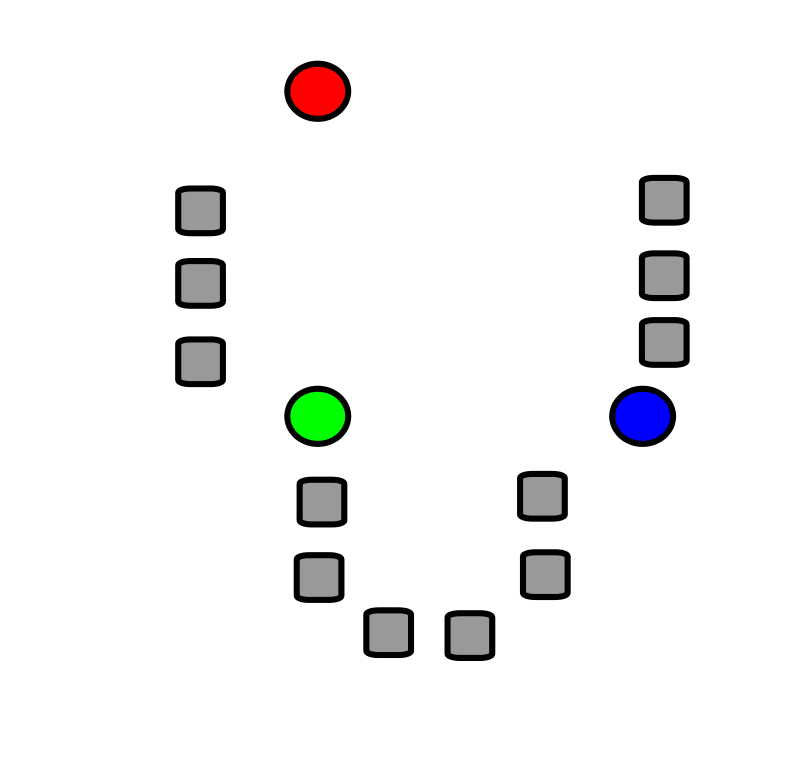
\includegraphics[width = .23\textwidth]{KMeans1.png}}\hspace{1em}%
    \subfloat[k clusters are created by associating every observation with the nearest mean. The partitions here represent the Voronoi diagram generated by the means.]{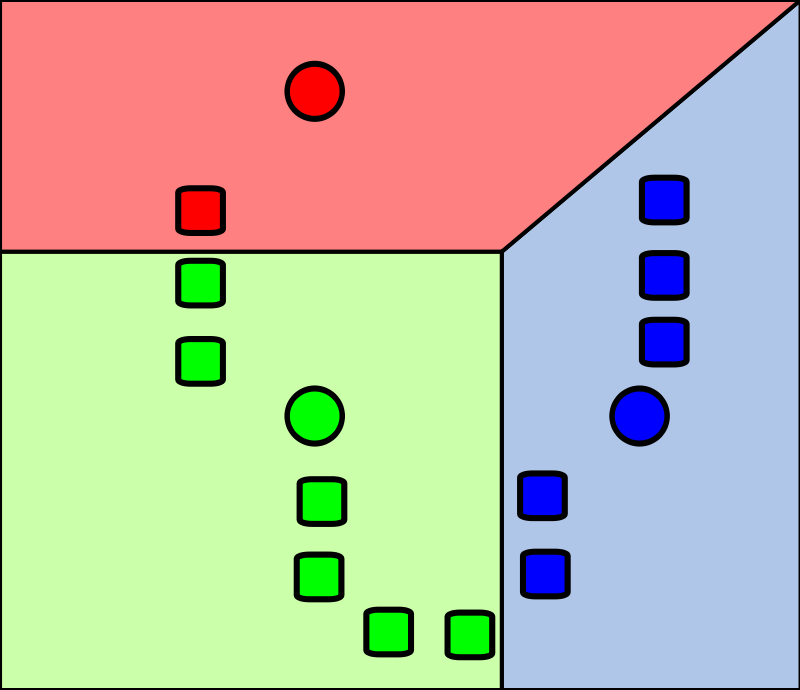
\includegraphics[width = .23\textwidth]{KMeans2.png}}\hspace{1em}%
    \subfloat[The centroid of each of the k clusters becomes the new mean]{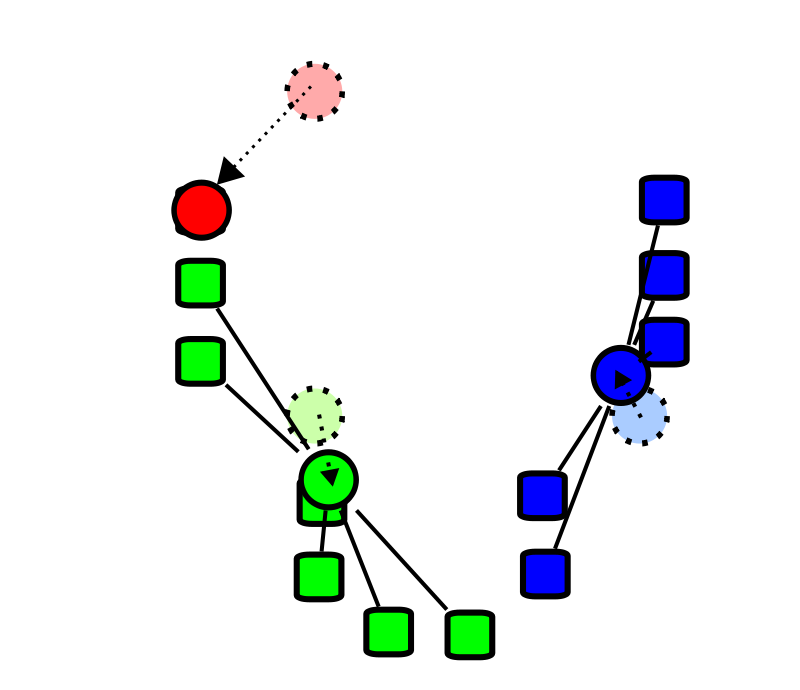
\includegraphics[width = .23\textwidth]{KMeans3.png}}\hspace{1em}%
    \subfloat[Steps 2 and 3 are repeated until convergence has been reached.]{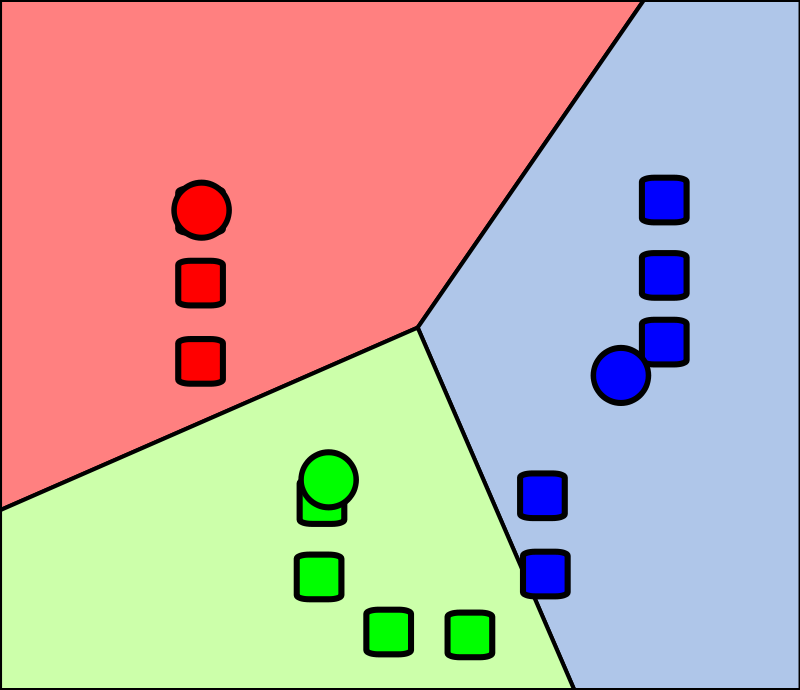
\includegraphics[width = .23\textwidth]{KMeans4.png}}% 
    \caption{Standard k-means clustering algorithm}
\end{figure}


%%%%%%%%%%%%%%%%%%%%%%%%%%%%%%%%%%%%%%%
%%%% WHAT I DID DURING THE SUMMERS %%%%
%%%%%%%%%%%%%%%%%%%%%%%%%%%%%%%%%%%%%%%
\chapter{What I did during the summers}
\markboth{}{}
\section{Literature}
Initial part of the internship was to read the literature available on the domain and do kind of a survey on the available modeling techniques. Some the techniques that I read about, have been documented in the introduction part. A summary of the all the surveyed techniques can be found here in this \href{http://slides.com/tminima/gene-regulatory-networks\#/}{online presentation}\footnote{http://slides.com/tminima/gene-regulatory-networks\#/} and \href{http://slides.com/tminima/modeling-grn-with-big-data\#/}{this one}\footnote{http://slides.com/tminima/modeling-grn-with-big-data\#/}.

\section{Working with microarray data}
As explained in the Introduction chapter, microarray data is a data containing the measurements of the expression levels of genes. The whole process has been documented in the \href{http://slides.com/tminima/deck\#/}{linked slide}\footnote{http://slides.com/tminima/deck\#/} but it's been explained further in the coming sections.

\subsection{Getting the data}
In any data mining (analysis) project the first goal is getting the data. \href{http://www.ncbi.nlm.nih.gov/}{NCBI}\footnote{http://www.ncbi.nlm.nih.gov/} supports and distributes a variety of open databases for the medical and scientific communities. The data requirements of the project were fulfilled by NCBI. We decided to do the study on the Alzheimer's Disease (AD) so, the dataset chosen for the study was - \href{http://www.ncbi.nlm.nih.gov/geo/query/acc.cgi?acc=GSE5281}{\textbf{Alzheimer's disease and the normal aged brain (steph-affy-human-433773)}}\footnote{http://www.ncbi.nlm.nih.gov/geo/query/acc.cgi?acc=GSE5281}.

\subsection{Dataset description}
As the title of the dataset suggests, it contains the expression values of certain parts of an AD and normal aged brain.
The dataset consists of 161 samples with 54675 genes in each thus, making the whole dataset of the size of 1GB. There are 74 control variables and 87 treatment variables (or affected variables, in this case) with sub-categories (table \ref{vartab}) among them, measured on the \textit{Affymetrix Human Genome U133 Plus 2.0 Array} which is the technology released on Nov 07, 2003. This dataset was made public on Jul 10, 2006.

\begin{table}[h]
    \centering
    \begin{tabular}{ |l|p{0.5\textwidth}| }
        \hline
        Arrays & Variable Type\\
        \hline
        GSM119615-88 & Control (EC-13, HIP-13, MTG-12, PC-13, SFG-11, VCX-12)\\  
        GSM238763, 91-98 & Affected (EC-10) \\
        GSM238799-808 & Affected (HIP-10) \\
        GSM238809-25 & Affected (MTG-16) \\
        GSM238826,27, 34-41 & Affected (PC-9) \\
        GSM238842-48, 51, 54-68, 70, 71 & Affected (SFG-23) \\
        GSM238872-75, 77, 941-953, 955, 963 & Affected (VCX-19)\\
        \hline
    \end{tabular}
    \caption{Summary of control and affected variables}
    \label{vartab}
\end{table}

More specifically, I worked on Affymetrix data (Affymetrix CEL-files). CEL files contains the 'raw' data produced at the end of the array scan. The format of the CEL file is an ASCII text file divided up into sections. The start of each section is defined by a line containing a section name enclosed in square braces. The section names are: "CEL", "HEADER", "INTENSITY", "MASKS", "OUTLIERS" and "MODIFIED". For more details on the sections \href{http://media.affymetrix.com/support/developer/powertools/changelog/gcos-agcc/cel.html}{this link}\footnote{http://media.affymetrix.com/support/developer/powertools/changelog/gcos-agcc/cel.html} from the Affymetrix DEveloper Network will be helpful.

\subsection{Working Environment}
R is a free software environment for statistical computing and graphics. I used R in a Linux environment (Elementary OS) for the whole duration of the project.

The majority of the R packages used in this project to analyze the microarray data are developed by the \href{http://www.bioconductor.org/}{Bioconductor}\footnote{http://www.bioconductor.org/}. The main packages used were - \texttt{affy, genefilter, limma, hgu133plus2.db, GO.db, GOstats, KEGG.db, simpleaffy}.

\subsection{Importing Data}
Below shows the code snippet which is responsible for importing the data in our R environment. All the comments (green coloured lines) will explain what the code will do. This will be the common pattern you'll notice in the whole document. The comments will explain the code. Other explanations will be provided in prose.

\begin{lstlisting}[language=R, caption=Data Importing]
# The function ReadAffy() reads in the raw data files, and stores the data
# as an AffyBatch object. By default, all CEL-files in the same directory
# are read.
library(affy)
dat <- ReadAffy()
print(dat)

# Output of the above statement.
# AffyBatch object
# size of arrays=1164x1164 features (83 kb)
# cdf=HG-U133_Plus_2 (54675 affyids)
# number of samples=161
# number of genes=54675
# annotation=hgu133plus2
# notes=
\end{lstlisting}

As can be seen in the above output of \texttt{print(dat)} statement the \texttt{affy package} binds our data in an object (named \texttt{dat} here) with certain metadata like the number of samples, number of genes in the dataset, annotation upon which our dataset is based on, etc. Thus, our data is imported in the environment with the above shown code.

\section{Pre-processing}
How preprocessing comes into play in this study was explained in the Introduction (section \ref{preprocess}). The technical description is given here.

\subsection{Quality Control}
The Affymetrix platform has a collection of QC metrics and accompanying guidelines that aid the identification of problematic arrays. Quality control of Affymetrix arrays is performed for raw data, i.e., imported CEL files (or \texttt{dat} object in our case).

Basic quality control for Affymetrix consists of checking for RNA degradation and examining the expression for control genes, scaling factors, percentage of present genes and the average background.

One strong indicator of the good quality of our dataset is that it has already been used in publications still the following QC checks were done.

\begin{lstlisting}[language=R, caption=Quality Control]
# Function AffyRNAdeg() from package Affy calculates RNA degradation.
# Other descriptives will be calculated using the
# function qc() from package simpleaffy.

library(affy)
library(simpleaffy)

# QC stats plot
aqc <- qc(dat)
plot(aqc)

# RNA degradation plot
# Sample a no. of colors from all available colors into cols
# distinct colors are equal to the no. of samples in dat object.
cols <- sample(colors(), nrow(pData(dat)))

deg <- AffyRNAdeg(dat)

# Plots the actual image using above colors,
png("rnadeg.png"), width=12, height=10, units="in", res=250)
plotAffyRNAdeg(deg, col=cols)
# A legend is added, for every array it holds one thin line
# colored using the above cols object.
legend(legend=sampleNames(dat), x="topleft", lty=1, cex=0.5, col=cols)
dev.off()
\end{lstlisting}

\begin{figure}[h]
    \centering
    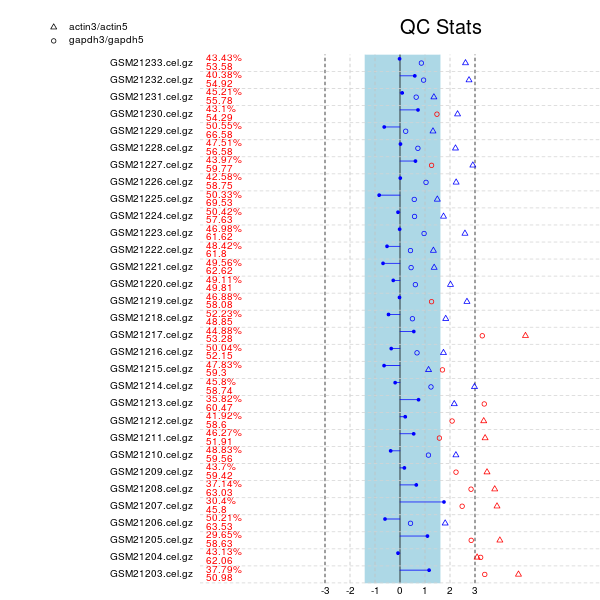
\includegraphics[scale=0.5]{qcplot.png}
    \caption{\texttt{Quality Control plot}}
    \captionsetup{singlelinecheck=off, font=footnotesize, width=\textwidth}
    \caption*{QC stats plot reports quality control parameters for the chips. The red numbers on the left report the number of probesets with present flag, and the average background on the chip. The blue region in the middle denotes the area where scaling factors are less than 3-fold of the mean scale factors of all chips. Bars that end with a point denote scaling factors for the chips. The triangles denote beta-actin 3’:5’ ratio, and open circles are GADPH 3’:5’ ratios. If the scaling factors or ratios fall within the 3-fold region (1.25-fold for GADPH), they are colored blue, otherwise red. The deviant chips are therefore easy to pick of by their red coloring. [note: this plot is not from the data used in this study as it was taking too much time to be generated.]}
\end{figure}

\begin{figure}[h]
    \centering
    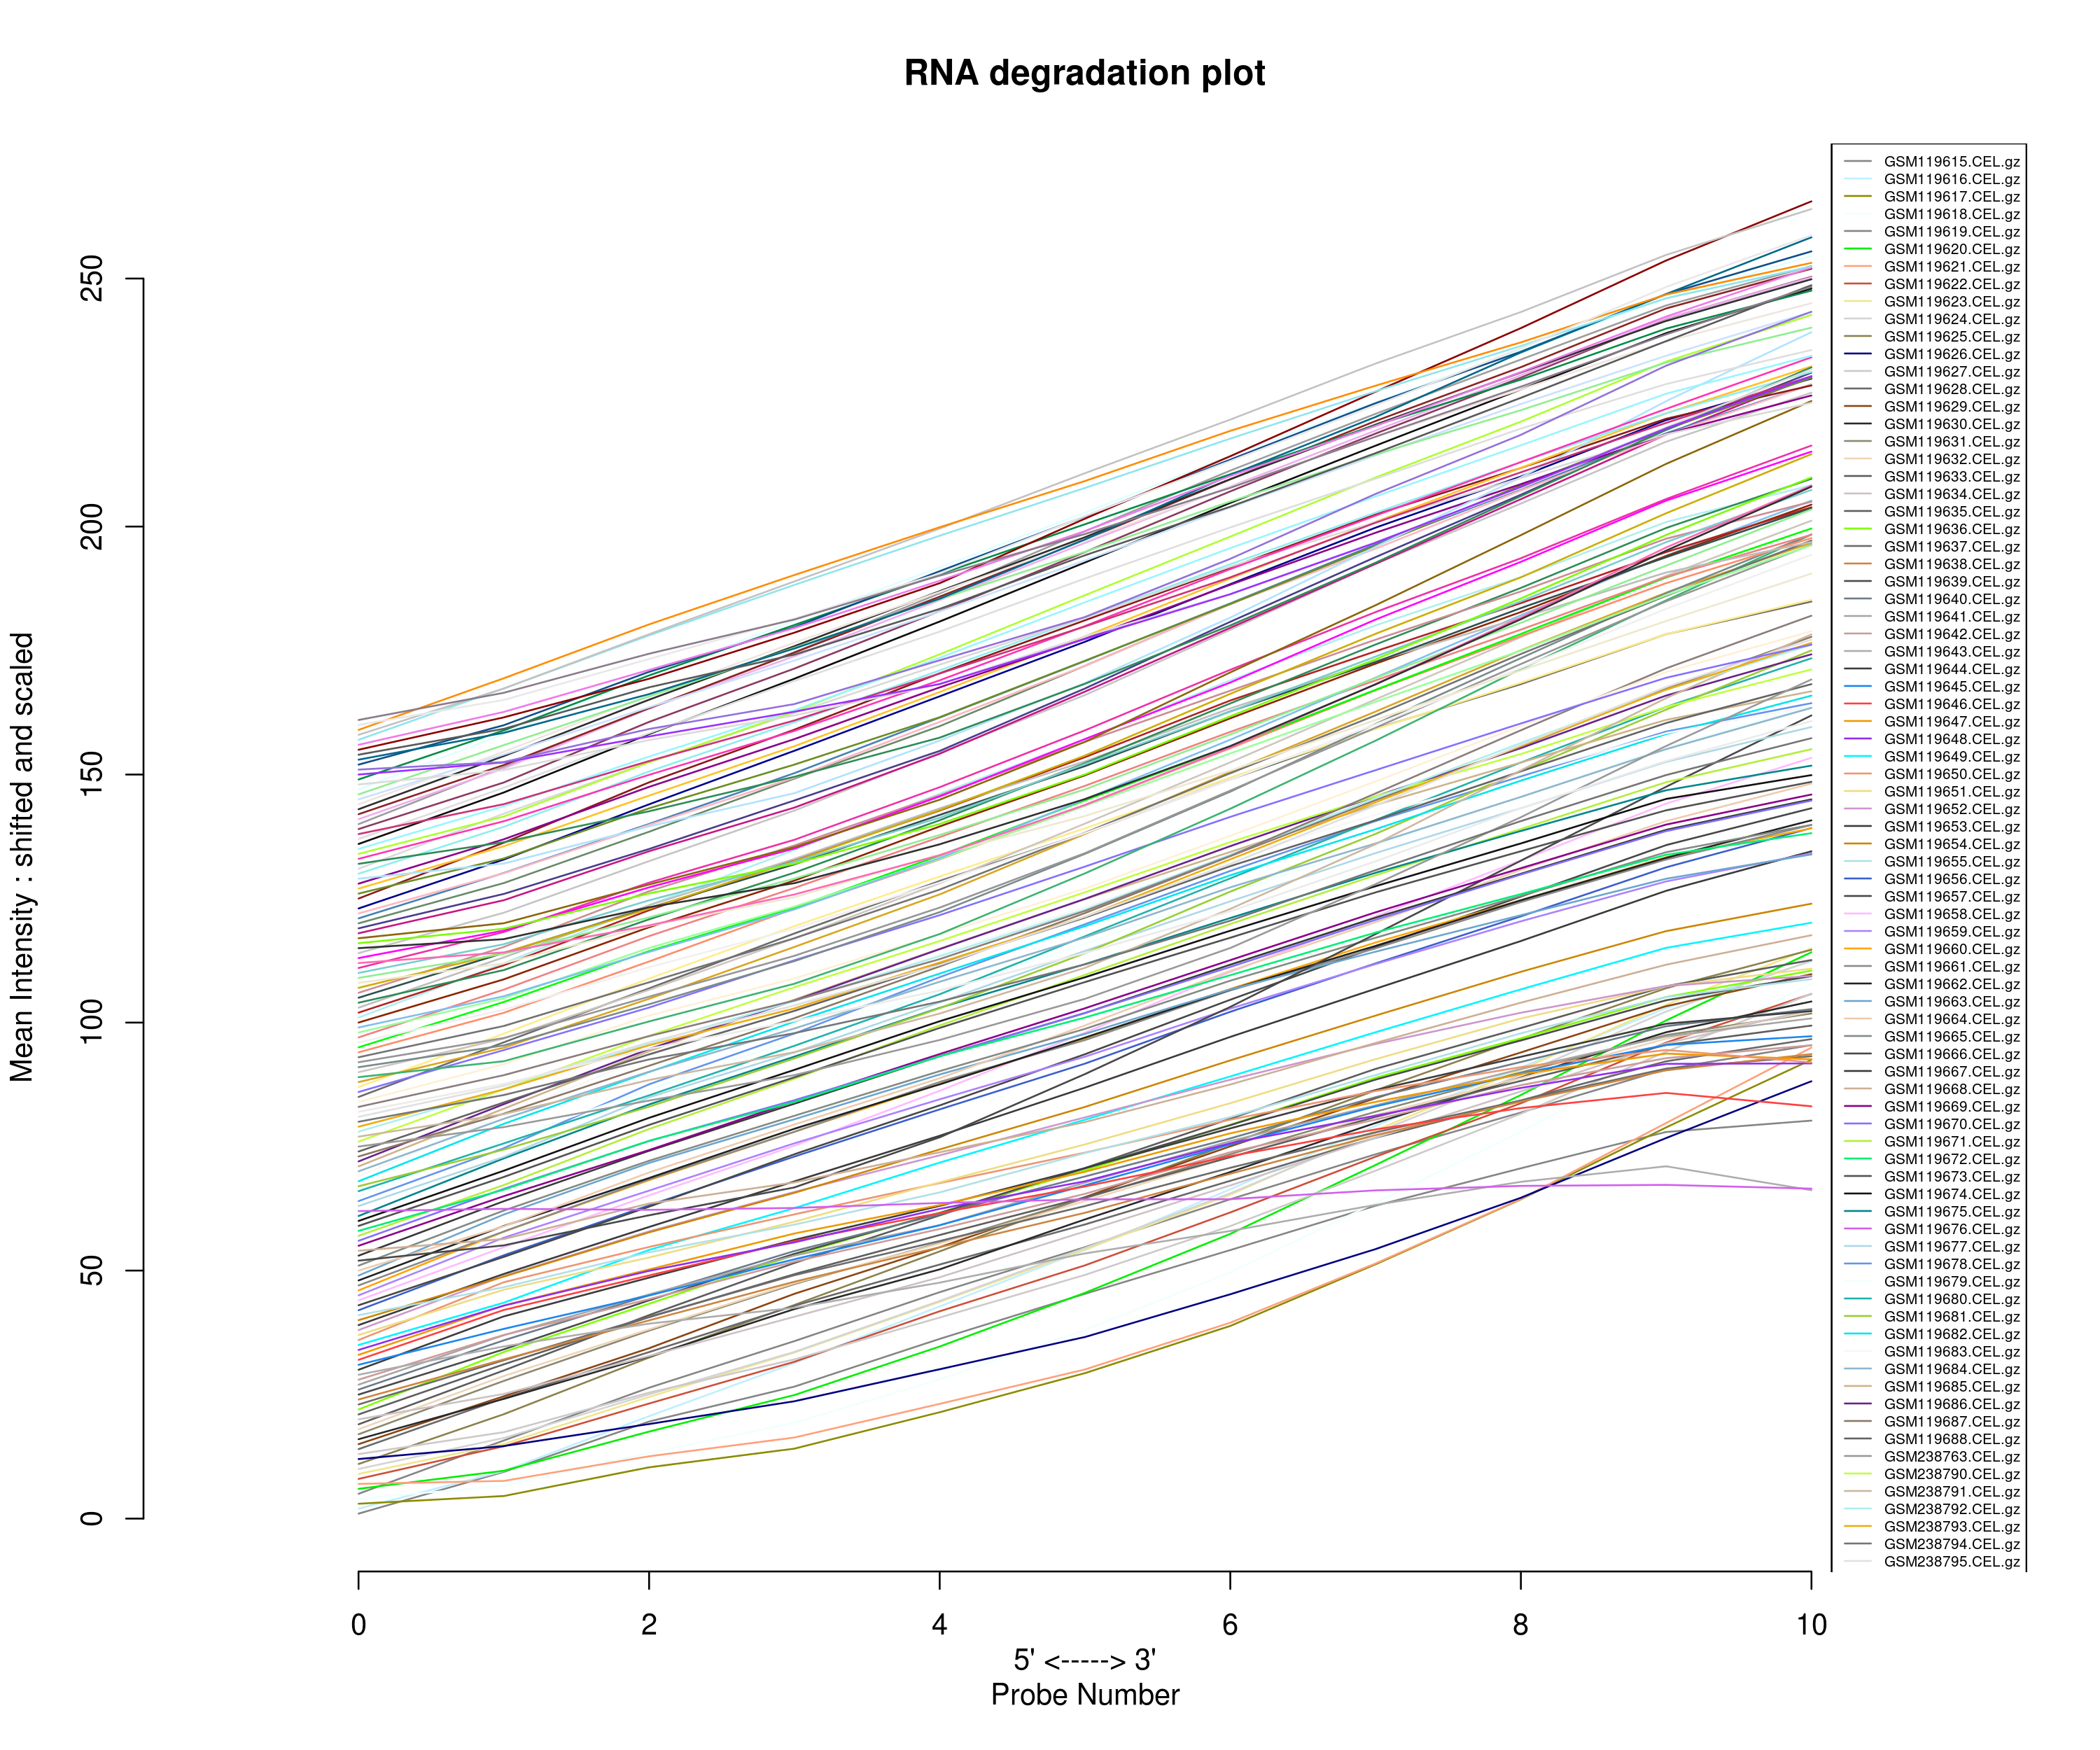
\includegraphics[scale=0.45]{rnadeg.png}
    \caption{\texttt{RNA degradation plot}}
    \captionsetup{singlelinecheck=off, font=footnotesize, width=\textwidth}
    \caption*{Every single array is represented by a single line. There are 161 lines. The idea is to check whether the slopes and profiles of the lines are similar for all the arrays. It is easy to spot the two lines that deviate from the others by having a steeper slope. Here, we have 3-4 lines at the bottom of the plot, with almost flat slope. Those arrays seems to be outliers, but it would probably not be too worrisome a phenomenan, and it is acceptable to retain them in the analysis.}
\end{figure}

\subsection{Normalization}
Robust multiarray average (RMA) is a commonly used method for pre-processing and normalizing Affymetrix data and our microarray data being Affymetrix type, natural choice was to use RMA. Another reason, why RMA was chosen is based on observations that it gives highly precise estimates of expression (which is desirable), although it might not give as accurate results (as it seems systematically to underestimate gene expression).

Typically pre-processing methods, such as RMA, consist of several steps: background correction, normalization of probes, and summarizing where individual probes are combined into a probeset. Also, log2-transformed data is used for further analysis. Thus, most of the normalization functions produce data in this format by default.

\begin{lstlisting}[language=R, caption=Data Normalization]
# Function rma() present in the package affy will be used here
# It takes in the raw data read previously.
dat2 <- rma(dat)

# Output:
# Background correcting
# Normalizing
# Calculating Expression

# The normalized data object (dat2) obtained here is in the format internal
# to the Bioconductor packages (affy). The following output of the dat2
# shows the fields it maintains about the data.

print(dat2)
# Output:
# ExpressionSet (storageMode: lockedEnvironment)
# assayData: 54675 features, 161 samples 
#   element names: exprs 
# protocolData
#   sampleNames: GSM119615.CEL.gz GSM119616.CEL.gz ... GSM238963.CEL.gz
#     (161 total)
#   varLabels: ScanDate
#   varMetadata: labelDescription
# phenoData
#   sampleNames: GSM119615.CEL.gz GSM119616.CEL.gz ... GSM238963.CEL.gz
#     (161 total)
#   varLabels: sample
#   varMetadata: labelDescription
# featureData: none
# experimentData: use 'experimentData(object)'
# Annotation: hgu133plus2

# Getting the normalized data in the matrix format
dat.m <- exprs(dat2)
print(dim(dat.m))
# Output: [1] 54675   161

# dat.m is the data object that will be used from now on,
# throughout the project.
# Removal of memory intensive objects
rm(dat, dat2)
\end{lstlisting}

\subsection{Filtering}
Here, we had to cases to consider- filtering before statistical testing and after statistical testing.

Statistical testing will be covered in the next section. Results of filtering process before and after statistical testing are documented here. There are two filtering methods considered here - standard deviation filter and expression filter. 

\subsubsection{Standard deviation filter}
Standard deviation for every single gene is calculated using the function \texttt{rowSds()}. After calculating these row-wise statistics, they are used for excluding the genes; we only retain those rows (genes) of the expression matrix that have a standard deviation of at least 2. The filtered dataset is saved in a new matrix called \texttt{dat.f}.

\begin{lstlisting}[language=R, caption=Standard Deviation Filtering]
library(genefilter)

# Standard deviation filter
# 1. Calculate the std deviation of every single gene
# 2. Retaining the genes with (sd >= 2)
std_filter <- function(analyzed_dat, fname){
    rsd <- rowSds(analyzed_dat)
    i <- rsd >= 2
    dat.f <- analyzed_dat[i,]

    print("Creating data dump... (dat.f.txt created)")
    write.table(dat.f,
        paste(fname, "dat.f.txt", sep=""),
        sep="\t",
        row.names=T,
        col.names=T,
        quote=F)

    rm(rsd, i)
    dat.f
}
\end{lstlisting}

\subsubsection{Expression Filtering}
When filtering by expression, it is not a sensible assumption that all arrays would behave similarly. On some arrays the gene might be expressed, but for some reason on some other arrays, it does not seem to be expressed at all or is expressed at a very low level. Therefore, the filter needs to take into account this possible discrepancy. This is implemented by letting the gene pass the filter (and to be included in the dataset), if the gene is expressed at the set level in at least some proportion of the samples. Using the functions \texttt{kOverA()} or \texttt{pOverA()} present in package \texttt{genefilter} we can make such filters. The former function uses the absolute number of samples during filtering, whereas the latter function uses the proportion. We will use the proportion method here (that is, \texttt{pOverA()} function).

Thus, to describe the process of filtering, first, a filtering function is created using the function \texttt{pOverA()} (line 15). This function is applied to all rows of the matrix using the function \texttt{genefilter()} (line 18). Here, the assumption was we want to find 2-fold over-expression (A=1), and that the gene has to be over-expressed in at least 50\% (p=0.5) of the arrays.

\begin{lstlisting}[language=R, caption=Expression Filtering]
library(genefilter)

# Expression filter
# Gene expressed at the set level is at least in some
# proportion of the samples.
# kOverA -> uses absolute no of samples
# pOverA -> uses the proportion
#
# 1. Choose a filtering function (pOverA in this case) assuming
#     a) Intensity of a gene should be above log2(100) in at least 25
#        percent of the samples.
#     b) Interquartile range of log2-intensities should be at least 0.5
#
exp_filter <- function(analyzed_dat, fname){
    f1 <- pOverA(A=log2(100), p=0.25)
    f2 <- function(x) (IQR(x) > 0.5)
    ff <- filterfun(f1, f2)
    i <- genefilter(analyzed_dat, ff)

    dat.fo <- analyzed_dat[i, ]

    print("Creating data dump... (dat.fo.txt created)")
    write.table(dat.fo,
        paste(fname, "dat.fo.txt", sep=""),
        sep="\t",
        row.names=T,
        col.names=T,
        quote=F)

    rm(f1, f2, ff, i)
    dat.fo
}

\end{lstlisting}

\subsubsection{Filtering before Statistical Testing}
Lets see what we got in the data opbects after filtering before the statistical testing.

\begin{lstlisting}[language=R, caption=Filtering before Statistical Testing]
dat.f <- std_filter(dat.m, "BeforeStatTest/StdFilter/")
print(dim(dat.f))
# Output: [1]  30 161

dat.fo <- exp_filter(dat.m, "BeforeStatTest/ExpFilter/")
print(dim(dat.fo))
# Output: [1] 8755  161

# Further statistical testing will be conducted on the data object dat.f and dat.fo.
\end{lstlisting}

The dimensions of the matrices \texttt{dat.f} and \texttt{dat.fo} printed by the function \texttt{dim()} shows us that out of 54,675 genes, only, 30 and 8,755 genes were filtered in \texttt{dat.f} and \texttt{dat.fo}, respectively.

\subsubsection{Filtering after Statistical Testing}
\begin{lstlisting}[language=R, caption=Filtering after Statistical Testing]
# Assuming the data object obtained after statistical testing is dat.s

dat.s.f <- std_filter(dat.s, "AfterStatTest/StdFilter/")
print(dim(dat.s.f))
# Output: [1]   3 161

dat.s.fo <- exp_filter(dat.s, "AfterStatTest/ExpFilter/")
print(dim(dat.s.fo))
# Output: [1] 4175  161

\end{lstlisting}

The dimensions of the matrices \texttt{dat.s.f} and \texttt{dat.s.fo} printed by the function \texttt{dim()} gives us the filtered genes out of 54,675 genes. Only 3 and 4,175 genes were filtered in \texttt{dat.s.f} and \texttt{dat.s.fo}, respectively.

\section{Statistical Analyses}
Moving on with the statistical testing using the \texttt{limma} package from Bioconductor project. In order to be able to use tools in limma package, one must be able to build a \textbf{model matrix} that describes the experiment. R comes with a command \texttt{model.matrix()} that makes building the model matrix a bit easier. The following code demonstrates that.

\begin{lstlisting}[language=R, caption=Design Matrix]
groups <- c(
    rep("C", 74),
    rep("T1", 10),
    rep("T2", 10),
    rep("T3", 16),
    rep("T4", 9),
    rep("T5", 23),
    rep("T6", 19))

# Creation of a model matrix.
groups <- as.factor(groups)
design <- model.matrix(~groups)
print(design)
# Output:
#     (Intercept) groupsT1 groupsT2 groupsT3 groupsT4 groupsT5 groupsT6
# 1             1        0        0        0        0        0        0
# 2             1        0        0        0        0        0        0
# 3             1        0        0        0        0        0        0
# 4             1        0        0        0        0        0        0
# 5             1        0        0        0        0        0        0
# 6             1        0        0        0        0        0        0
# ...
# 154           1        0        0        0        0        0        1
# 155           1        0        0        0        0        0        1
# 156           1        0        0        0        0        0        1
# 157           1        0        0        0        0        0        1
# 158           1        0        0        0        0        0        1
# 159           1        0        0        0        0        0        1
# 160           1        0        0        0        0        0        1
# 161           1        0        0        0        0        0        1
# attr(,"assign")
# [1] 0 1 1 1 1 1 1
# attr(,"contrasts")
# attr(,"contrasts")$groups
# [1] "contr.treatment"

\end{lstlisting}

\subsection{Analyses using linear model}
Empirical bayes analysis is carried out by using the command \texttt{lmFit()} (line 30) followed by \texttt{eBayes()} (line 31). The object, \texttt{fit} contains the results of the analysis. Results can be extracted using the command \texttt{toptable()}.

\begin{lstlisting}[language=R, caption=Statistical Testing]
# Assumption: Data is normally distributed. Thus, using linear models.
# From a typical Affymetrix experiment, maybe only about
# 20% of the expression values are normally distributed.
# One should probably use non-parametric methods for the analysis
library(limma)

# Groups and model matrix were created by the data.R
# On filtered data
analysis <- function(filter_dat, fname){
    fit <- lmFit(filter_dat, design)
    fit <- eBayes(fit)

    # Extracting the genes that have the unadjusted p-value at most 0.001
    #  TODO: Think about the other values of coeff.
    tt <- toptable(fit, coef=2, n=nrow(filter_dat))
    rn <- rownames(tt)[tt$P.Value <= 0.001]
    # rn <- as.numeric(rn)
    dat.s <- filter_dat[rn, ]
    print("Dumping dat.s...")

    write.table(dat.s,
        paste(fname, "dat.s.txt", sep=""),
        sep="\t",
        row.names=T,
        col.names=T,
        quote=F)

    rm(fit, tt, rn)
    dat.s
}

# Analysis after the filtering was done in the previous section
# Analysis of dat.f (obtained after standard filtering).
dat.s1 <- analysis(dat.f, "BeforeStatTest/StdFilter/")
print(dim(dat.s1))
# Output: [1]   3 161

# Analysis of dat.fo (obtained after expression filtering).
dat.s2 <- analysis(dat.fo, "BeforeStatTest/ExpFilter/")
print(dim(dat.s2))
# Output: [1] 4138  161

# Analysis before the filtering.
dat.s <- analysis(dat.m, "AfterStatTest/")
print(dim(dat.s))
# Output: [1] 13949   161
\end{lstlisting}

The original values of all the genes that have the unadjusted p-value at most 0.001 after the statistical testing were extracted at lines 35-38. The object \texttt{dat.s} stores the data for the genes that were selected (as differentially expressed). As the output of \texttt{dim()} suggests, reduced from 54,675 genes we have 3 and 4138 genes in \texttt{dat.s1} and \texttt{dat.s2}, respectively. And, in \texttt{dat.s} (data object obtained after directly analysing \texttt{dat.m}), 54,675 genes were reduced to 13,949 genes.

\subsection{Gene Set Enrichment Analysis (GSEA)}
Before any analysis, microarray probe IDs need to be converted to \textbf{EntrezIDs}. EntrezIDs are gene-specific identifiers used by NCBI to cross-link different databases together. Annotation packages produced in the Bioconductor project contain the mappings from probe IDs to EntrezIDs.

\begin{lstlisting}[language=R, caption=Gene Set Enrichment Analysis]
# Gene Set Enrichment Analysis
# Works on filtered data

# source("http://www.bioconductor.org/biocLite.R")
# biocLite("hgu133plus2.db")
library(hgu133plus2.db)

gsea <- function(dat, fname){
    allg <- get("hgu133plus2ENTREZID")
    allg <- as.data.frame(unlist(as.list(allg)))
    # Contains all the probes that we consider interesting
    myids <- unique(allg[rownames(dat),])

    print("Dumping myids...")
    write.table(myids,
        paste(fname, "myids.txt", sep=""),
        sep="\t",
        row.names=T,
        col.names=T,
        quote=F)

    rm(allg)
    myids
}

# Gene set enrichment analysis before statistical testing
# IDs from dat.s2 (obtained after standard filtering).
myids1 <- gsea(dat.s1, "BeforeStatTest/StdFilter/")
print(length(myids1))
# Output: [1] 2

# IDs from dat.s2 (obtained after expression filtering).
myids2 <- gsea(dat.s2, "BeforeStatTest/ExpFilter/")
print(length(myids2))
# Output: [1] 3244

# Gene set enrichment analysis after statistical testing
myids.s.1 <- gsea(dat.s.f, "AfterStatTest/StdFilter/")
print(length(myids.s.1))
# Output: [1] 2

myids.s.2 <- gsea(dat.s.fo, "AfterStatTest/ExpFilter/")
print(length(myids.s.1))
# Output: [1] 3269

\end{lstlisting}

In the above code, the annotation package \texttt{hgu133plus2} was loaded and then all the \texttt{ENTREZID} are loaded in a data frame \texttt{allg} followed by the keeping the unique EntrezIDs only for the genes in our list of interesting genes (data object obtained after the statistical analysis). Now \texttt{myids} contains all the probes that we considered interesting.

As can be seen, in the datset obtained after filtering before statistical analysis, out of 3 genes in dat.s1 we got 2 interesting genes (saved in myids1) and out of 4138 there are 3244 genes (saved in myids2). Although, the results of standard deviation filtered dataset doesn't give many interested genes we'll try to see what we get in the further use of this data object. The similar pattern in seen in the dataset obtained after the filtering after statistical testing (output of the code shows the numbers).

\subsubsection{GO categories}
The actual test is run in three steps, since the GO hierarchy consists of three distinct ontologies - \textit{biological process} (BP), \textit{molecular function} (MF) and \textit{cellular component} (CC).

First the hypergeometric test parameters are initialized using the command \texttt{new()} (with arguments, \texttt{geneIds}: names of the interesting genes, \texttt{annotation}: an annotation
package, \texttt{ontology}: which ontology to test, \texttt{pvalueCutoff}: p-value cutoff, \texttt{testDirection}: whether to test over- or under-enrichment). After initialization, the test is calculated using the command \texttt{hyperGTest()}.
The following commands test all three ontologies, and store the results in objects \texttt{resultBP, resultMF and resultCC}. They all use the p-value of 0.05, which is a rather typical choice, and test for over-enrichment, which is also a typical choice. A HTML report was generated using \texttt{htmlReport()}.
\newline

\begin{lstlisting}[language=R, caption=Gene Set Enrichment Analysis - GO categories]
library(GO.db)
library(GOstats)

GO <- function(myids, fname){
    params <- new("GOHyperGParams",
        geneIds=myids,
        annotation=c("hgu133plus2"),
        ontology="BP",
        pvalueCutoff=0.05,
        conditional=FALSE,
        testDirection="over")
    resultBP <- hyperGTest(params)
    params <- new("GOHyperGParams",
        geneIds=myids,
        annotation=c("hgu133plus2"),
        ontology="MF",
        pvalueCutoff=0.05,
        conditional=FALSE,
        testDirection="over")
    resultMF <- hyperGTest(params)
    params <- new("GOHyperGParams",
        geneIds=myids,
        annotation=c("hgu133plus2"),
        ontology="CC",
        pvalueCutoff=0.05,
        conditional=FALSE,
        testDirection="over")
    resultCC <- hyperGTest(params)

    fname <- paste(fname, "hypergeo_GO.html", sep="")
    htmlReport(resultBP, fname, append=T)
    htmlReport(resultMF, fname, append=T)
    htmlReport(resultCC, fname, append=T)
    print("Created the HTML report...")

    rm(params, fname)
    result <- list(resultBP = resultBP,
        resultMF = resultMF,
        resultCC = resultCC)
}

# Analysis before the stat test was done.
GO_result1 <- GO(myids1, "BeforeStatTest/StdFilter/")
# Output:
# Error in getGoToEntrezMap_db(p) : 
#   The genes you are testing do not have any corresponding GO terms for the ontology you are searching.

GO_result2 <- GO(myids2, "BeforeStatTest/ExpFilter/")
print(GO_result2)
# $resultBP
# Gene to GO BP  test for over-representation 
# 7966 GO BP ids tested (1114 have p < 0.05)
# Selected gene set size: 2815 
#     Gene universe size: 14686 
#     Annotation package: hgu133plus2 
# 
# $resultMF
# Gene to GO MF  test for over-representation 
# 2051 GO MF ids tested (267 have p < 0.05)
# Selected gene set size: 2759 
#     Gene universe size: 14312 
#     Annotation package: hgu133plus2 
# 
# $resultCC
# Gene to GO CC  test for over-representation 
# 1059 GO CC ids tested (301 have p < 0.05)
# Selected gene set size: 2986 
#     Gene universe size: 15586 
#     Annotation package: hgu133plus2

# Analysis after the stat test.
GO_result.s.1 <- GO(myids.s.1, "AfterStatTest/StdFilter/")
# Error in getGoToEntrezMap_db(p) : 
#   The genes you are testing do not have any corresponding GO terms for the ontology you are searching.

GO_result.s.2 <- GO(myids.s.2, "AfterStatTest/ExpFilter/")
# $resultBP
# Gene to GO BP  test for over-representation 
# 7985 GO BP ids tested (1123 have p < 0.05)
# Selected gene set size: 2838 
#     Gene universe size: 14686 
#     Annotation package: hgu133plus2 
# 
# $resultMF
# Gene to GO MF  test for over-representation 
# 2051 GO MF ids tested (260 have p < 0.05)
# Selected gene set size: 2781 
#     Gene universe size: 14312 
#     Annotation package: hgu133plus2 
# 
# $resultCC
# Gene to GO CC  test for over-representation 
# 1057 GO CC ids tested (303 have p < 0.05)
# Selected gene set size: 3011 
#     Gene universe size: 15586 
#     Annotation package: hgu133plus2
\end{lstlisting}

As expected, due to very few (only 2) interesting genes there were no satisfactory results obtained for the GO categories in the case of \texttt{myids1} (IDs obtained out of the data from data filtered using standard deviation filter, before statistical analysis). In fact, it ended with an error. Now, the GO results of the dataset after expression filtering we got some considerable matches, as the output shows.

The dataset obtained after filtering after the statistical testing follows a similar pattern. The standard filter doesn't show much promise, but the expression filter gave some good results.

\begin{figure}[h]
    \centering
    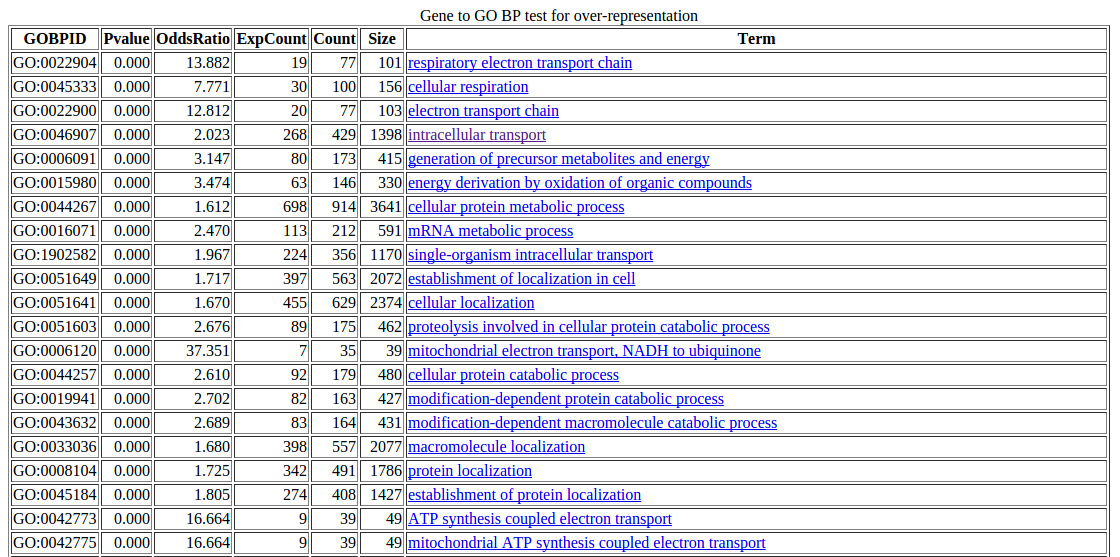
\includegraphics[width=\textwidth]{GOreport.png}
    \caption {\texttt{A snapshot of the HTML report generated}, clicking on a link, will take you to the particular entry in the genome database with all the onlology details.}
\end{figure}

\subsubsection{KEGG pathways}
Analysis for KEGG pathways is very similar to the one explained for the GO categories. Prior to the test, we need to generate a list of EntrezIDs (saved in the object \texttt{myids}). The end result is the generation of the HTML report.

\begin{lstlisting}[language=R, caption=Gene Set Enrichment Analysis - KEGG pathways]
library(KEGG.db)

KEGG <- function(myids, fname) {
    params <- new("KEGGHyperGParams",
        geneIds=myids,
        annotation="hgu133plus2",
        pvalueCutoff=0.05,
        testDirection="over")
    result <- hyperGTest(params)

    fname <- paste(fname, "hypergeo_KEGG.html", sep="")
    htmlReport(result, fname, append=T)
    print("HTML report generated...")

    rm(params, fname)
    result
}

# Analysis before the stat test
KEGG_result1 <- KEGG(myids1, "BeforeStatTest/StdFilter/")
# Output:
#Warning messages:
#1: No results met the specified criteria.  Returning 0-row data.frame 
#2: In htmlReportFromDf(r = df, caption = paste(label, description(r)),  :
#  No rows to report.  Skipping

KEGG_result2 <- KEGG(myids2, "BeforeStatTest/ExpFilter/")
print(KEGG_result2)
# Output:
# Gene to KEGG  test for over-representation 
# 210 KEGG ids tested (37 have p < 0.05)
# Selected gene set size: 1152 
#     Gene universe size: 5234 
#     Annotation package: hgu133plus2

# Analysis after the stat test.
KEGG_result.s.1 <- KEGG(myids.s.1, "AfterStatTest/StdFilter/")
# Warning messages:
# 1: No results met the specified criteria.  Returning 0-row data.frame 
# 2: In htmlReportFromDf(r = df, caption = paste(label, description(r)),  :
#   No rows to report.  Skipping

KEGG_result.s.2 <- KEGG(myids.s.2, "AfterStatTest/ExpFilter/")
# Gene to KEGG  test for over-representation 
# 210 KEGG ids tested (38 have p < 0.05)
# Selected gene set size: 1162 
#     Gene universe size: 5234 
#     Annotation package: hgu133plus2
\end{lstlisting}

Here again, the standard deviation filtered data didn't have any matching KEGG pathway, while the the expression filtered data did give us results.

% \subsection{Gene Set Testing (GST)}
% In GST genes are first assigned to pathways or categories and their statistical significance is tested using both the knowledge of the category and the expression data. It takes the original, unfiltered data as it came out after the normalization (data object \texttt{dat.m}).

% \subsubsection{GO categories}
% \begin{lstlisting}[language=R, caption=Gene Set Testing - GO categories]
% \end{lstlisting}

% \subsubsection{KEGG pathways}
% \begin{lstlisting}[language=R, caption=Gene Set Testing - KEGG pathways]
% \end{lstlisting}

\section{Clustering}
\subsection{Heatmap or Hierarchical Clustering}
As the introducition said, heatmap presents hierarchical clustering of both genes and arrays (that is 161 experiments in our data set), and additionally displays the expression patterns, all in the same visualization.

Library \texttt{amap} offers function \texttt{hcluster()} to calculate the distances using person correlation (argument \texttt{method="pearson"}) and linkage criteria as average linkage (argument \texttt{link="average"}). The  heatmap can be generated using the command \texttt{heatmap()}.

\begin{lstlisting}[language=R, caption=Heatmap \& Hierarchical Clustering]
# We are going to use the filtered or analysed data (dat.f or dat.s) for clustering.

# Function hcluster() from package amap can calculate the
# both the distances and the tree construction details.
# We will use Pearson coorelation for the distances and
# Average Linkage as the tree construction method. Other
# methods can be used by changing the arguments as follows,
# method="euclidean" or method="spearman"
# link="complete" or link="single"
library(amap)

cluster <- function(dat, fname){
    clust.genes <- hcluster(x=dat, method="pearson", link="average")
    clust.arrays <- hcluster(x=t(dat), method="pearson", link="average")

    # Usual coloring scheme for microarray data in heatmaps is to
    # present down-regulated genes with green, and up-regulated genes with red.
    # Function colorRampPalette() takes first argument as the color for the
    # smallest observation (the most down-regulated gene), and second argument
    # the color for the largest observation (the most up-regulated gene). The
    # number after the command specifies how many different colors between the
    # extremes should be generated, here we use 32 colors.
    heatcol <- colorRampPalette(c("Green", "Red"))(32)

    # Function heatmap() generates the heatmap. It takes in 4 arguments
    # x = matrix dataset (dat.m is converted to matrix here)
    # Rowv = dendogram of clustred genes
    # Colv = dendogram of clustred samples
    # col = coloring scheme to be used

    png(paste(fname, "heatmap.png"), width=12, height=10, units="in", res=250)
    heatmap(x=as.matrix(dat),
        Rowv=as.dendrogram(clust.genes),
        Colv=as.dendrogram(clust.arrays),
        col=heatcol)
    dev.off()

    rm(clust.genes, clust.arrays, heatcol)
}

# Clustering before the stat test
# Standard deviation filtered data
cluster(dat.f, "BeforeStatTest/StdFilter/")
# Statistically analysed, standard deviation data
cluster(dat.s1, "BeforeStatTest/StdFilter/stat_")
# Expression based filtered data
cluster(dat.fo, "BeforeStatTest/ExpFilter/")
# Statistically analysed, expression based filtered data
cluster(dat.s2, "BeforeStatTest/ExpFilter/stat_")

# Clustering after the stat test
# Statistically analyzed data
cluster(dat.s, "AfterStatTest/")
# Standard deviation filtered data
cluster(dat.s.f, "AfterStatTest/StdFilter/")
# Expression based filtered data
cluster(dat.s.fo, "AfterStatTest/ExpFilter/")
\end{lstlisting}

Hierarchical clustering of genes are on the left side (with labeling on the right) and arrays are on the top of the colored area (with array labels at the bottom). In the colored area, every gene is represented by a colored bar. Colors represent the down-regulation (green) or up-regulation (red) of the genes.

\begin{figure}[h]
    \centering
    \subfloat[Standard deviation filtered data clustering]{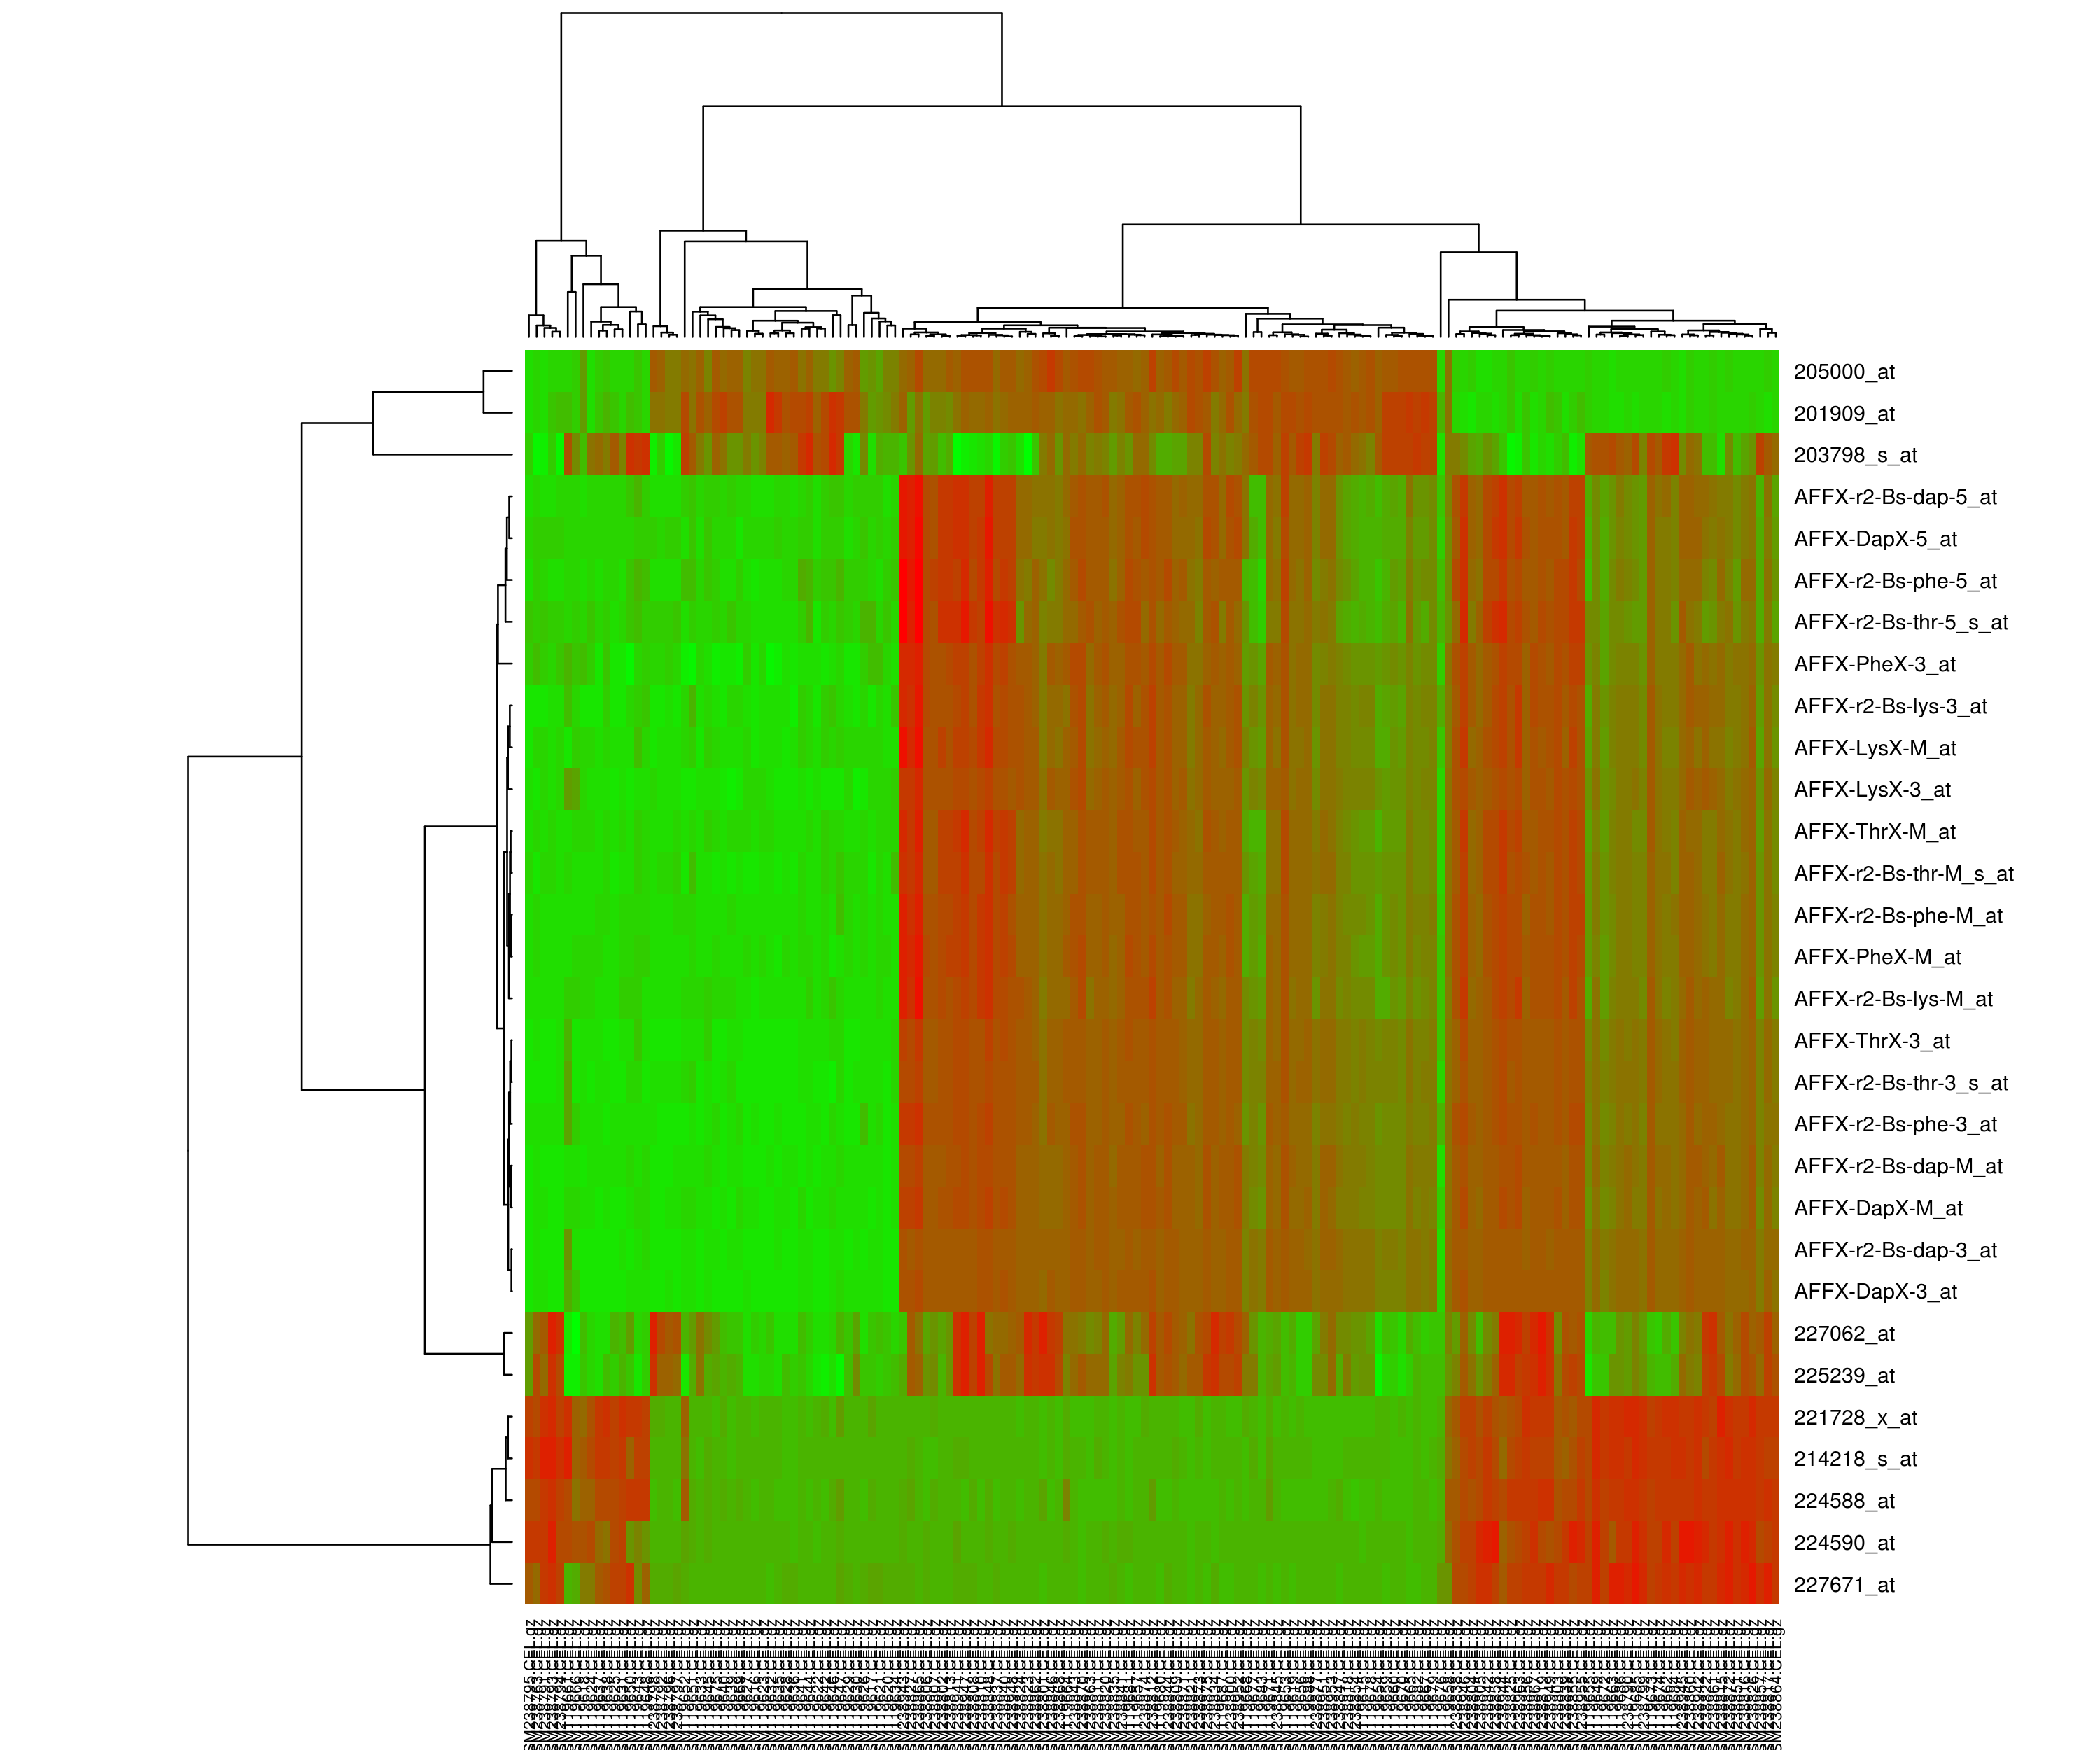
\includegraphics[width = .48\textwidth]{b_heatmap_f.png}}\hspace{1em}%
    \subfloat[Statistically analysed, standard deviation data clustering]{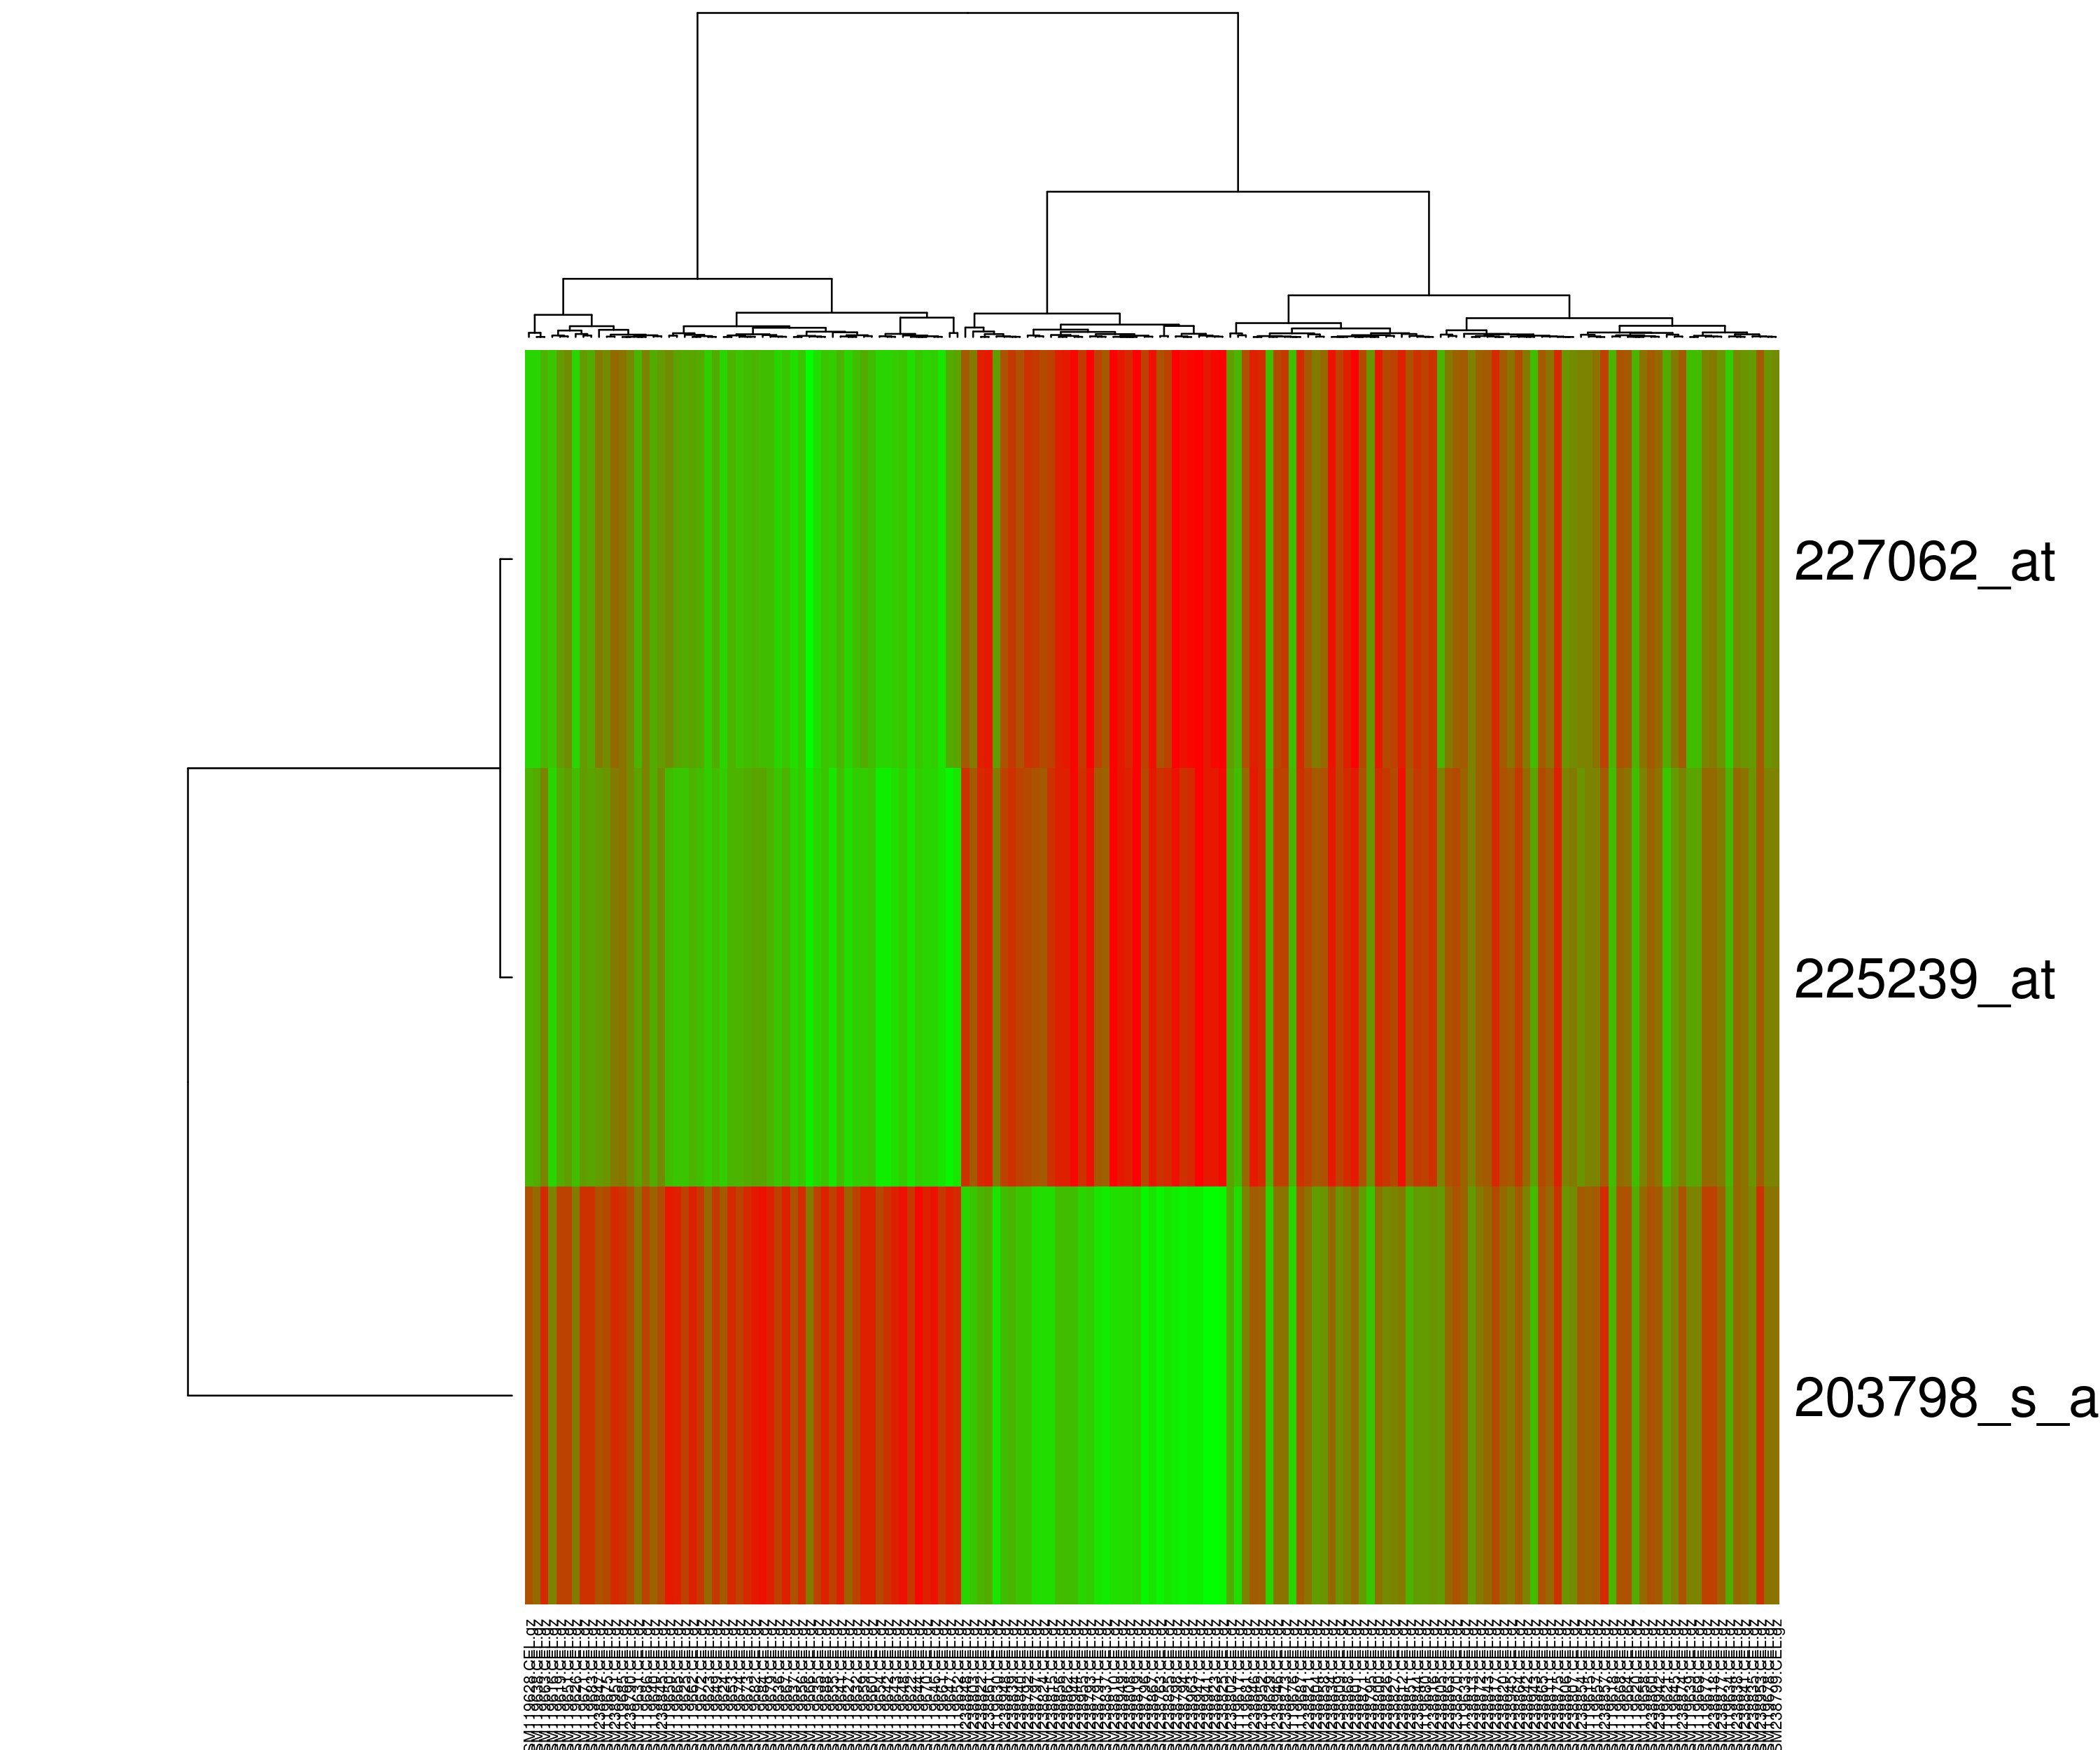
\includegraphics[width = .48\textwidth]{b_heatmap_s.png}}\hspace{1em}\\%
    \subfloat[Expression based filtered data clustering]{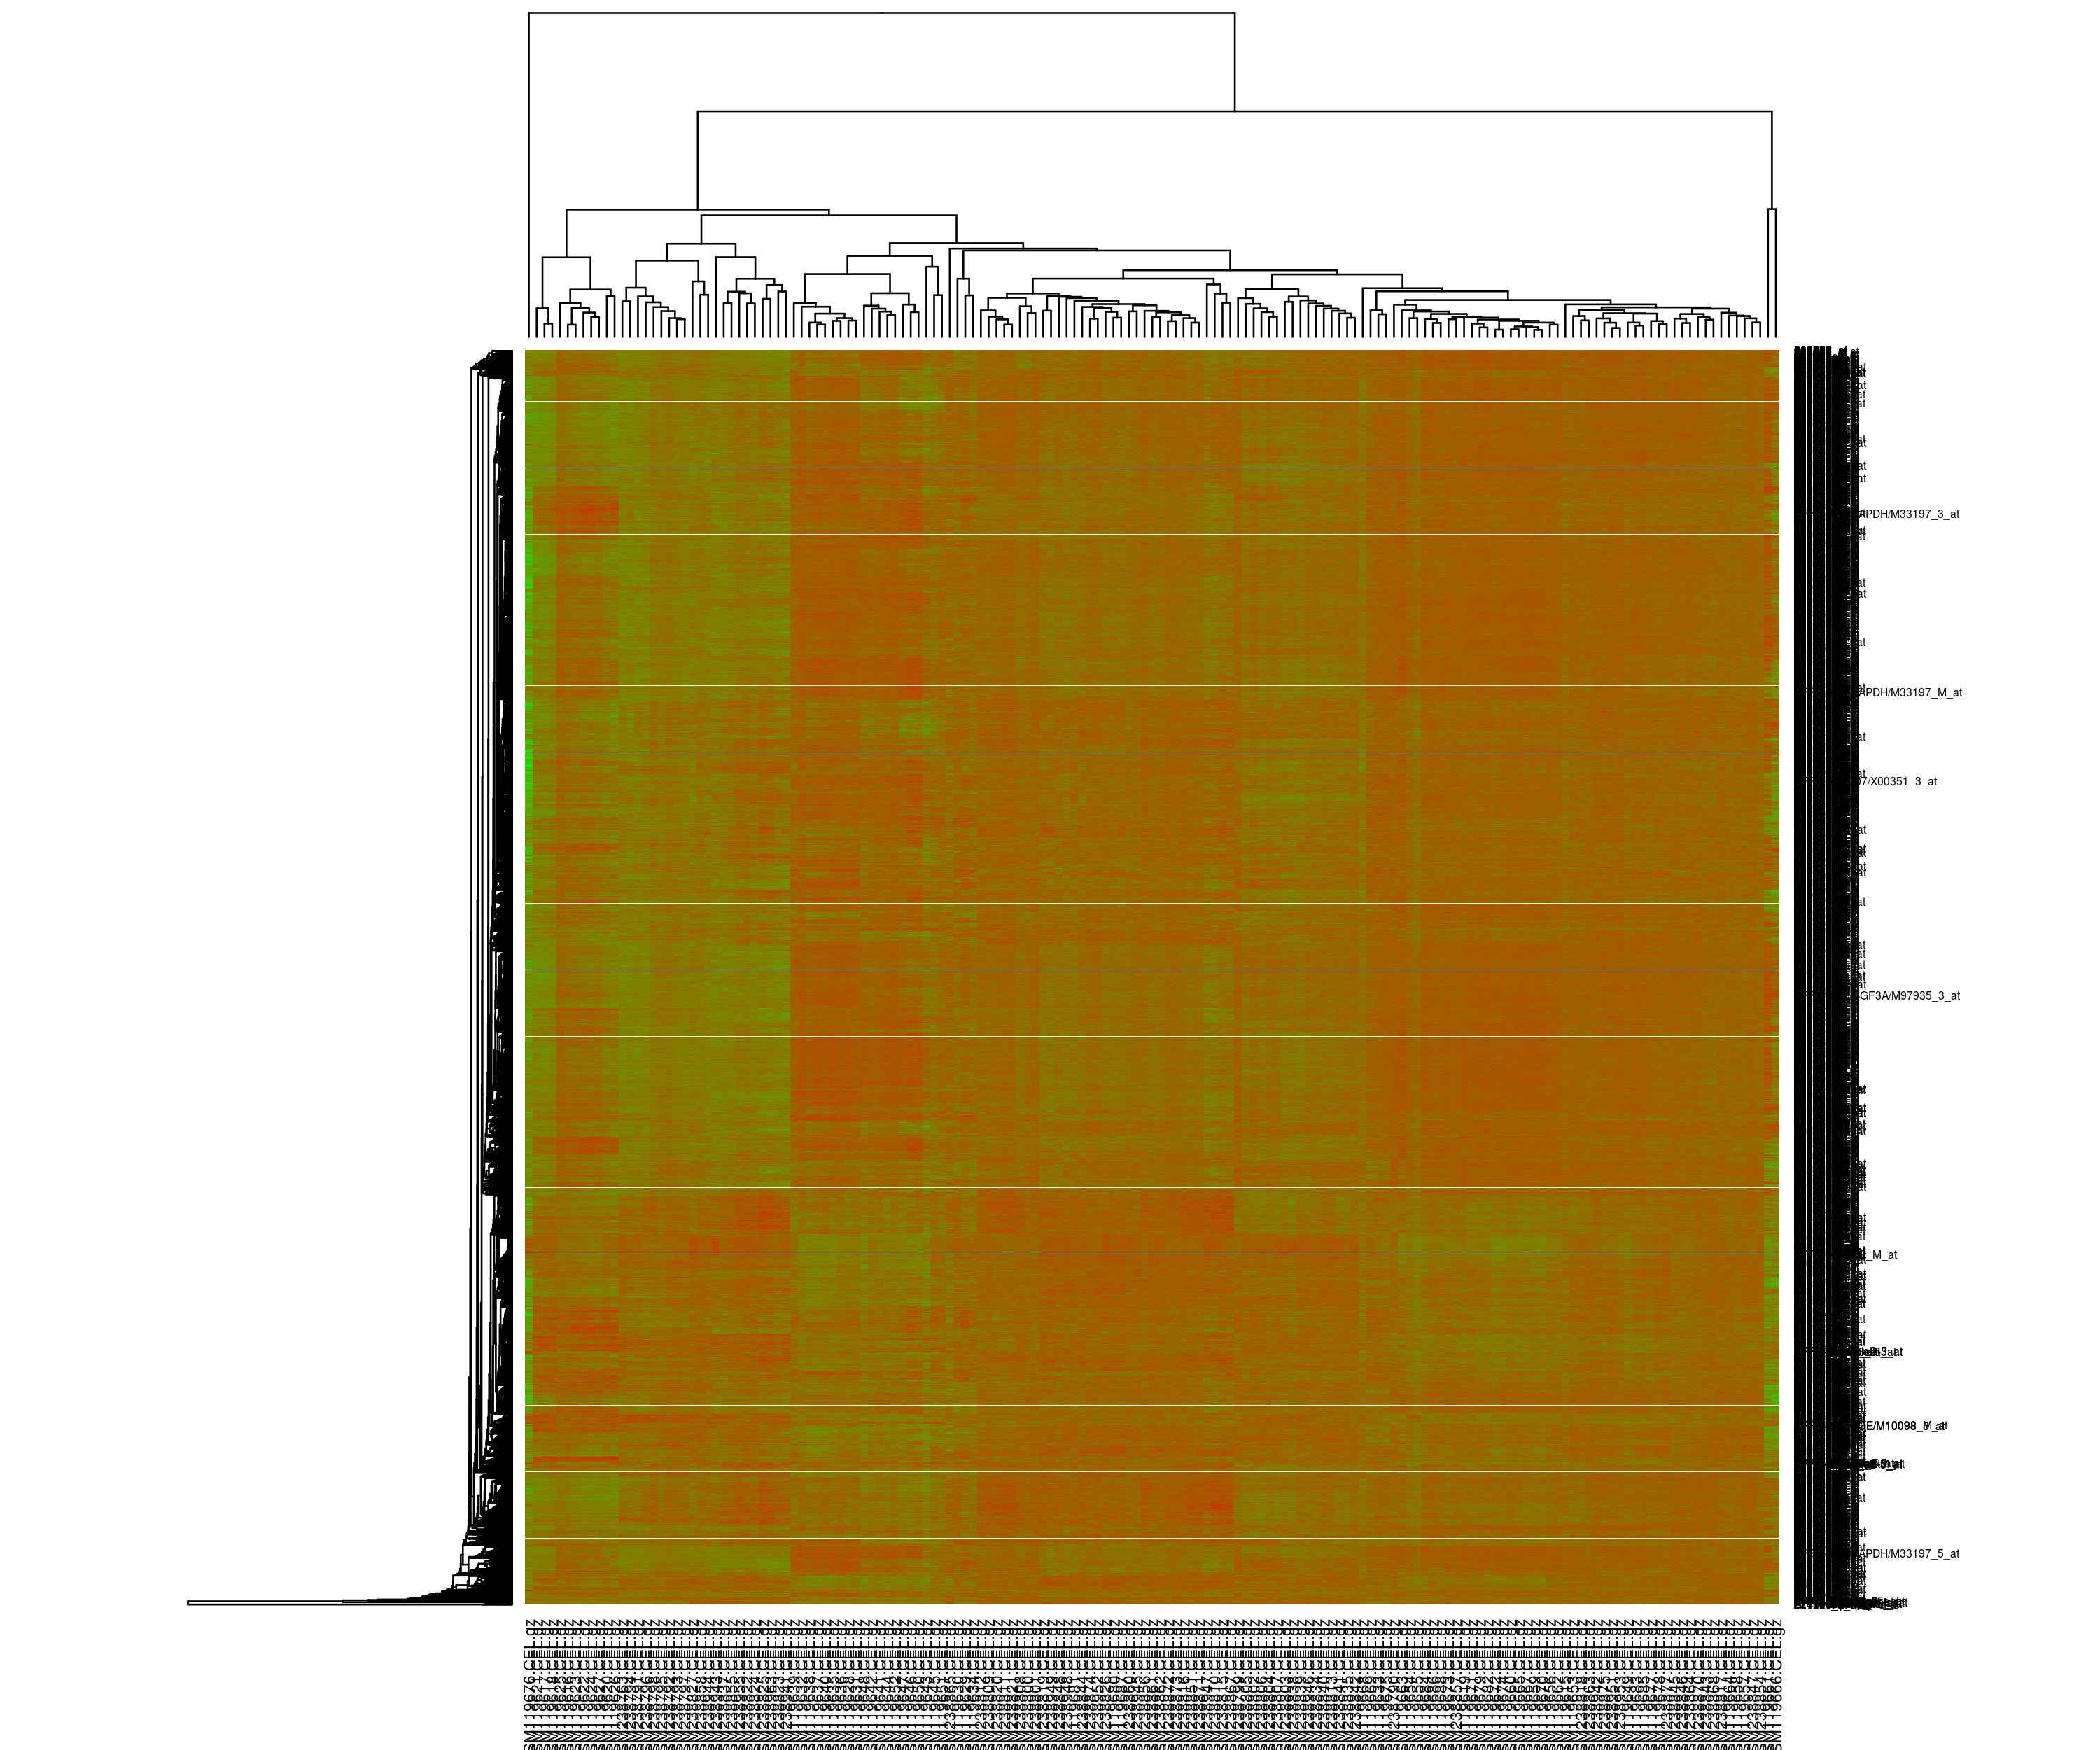
\includegraphics[width = .48\textwidth]{a_heatmap_f.png}}\hspace{1em}%
    \subfloat[Statistically analysed, expression based filtered data clustering]{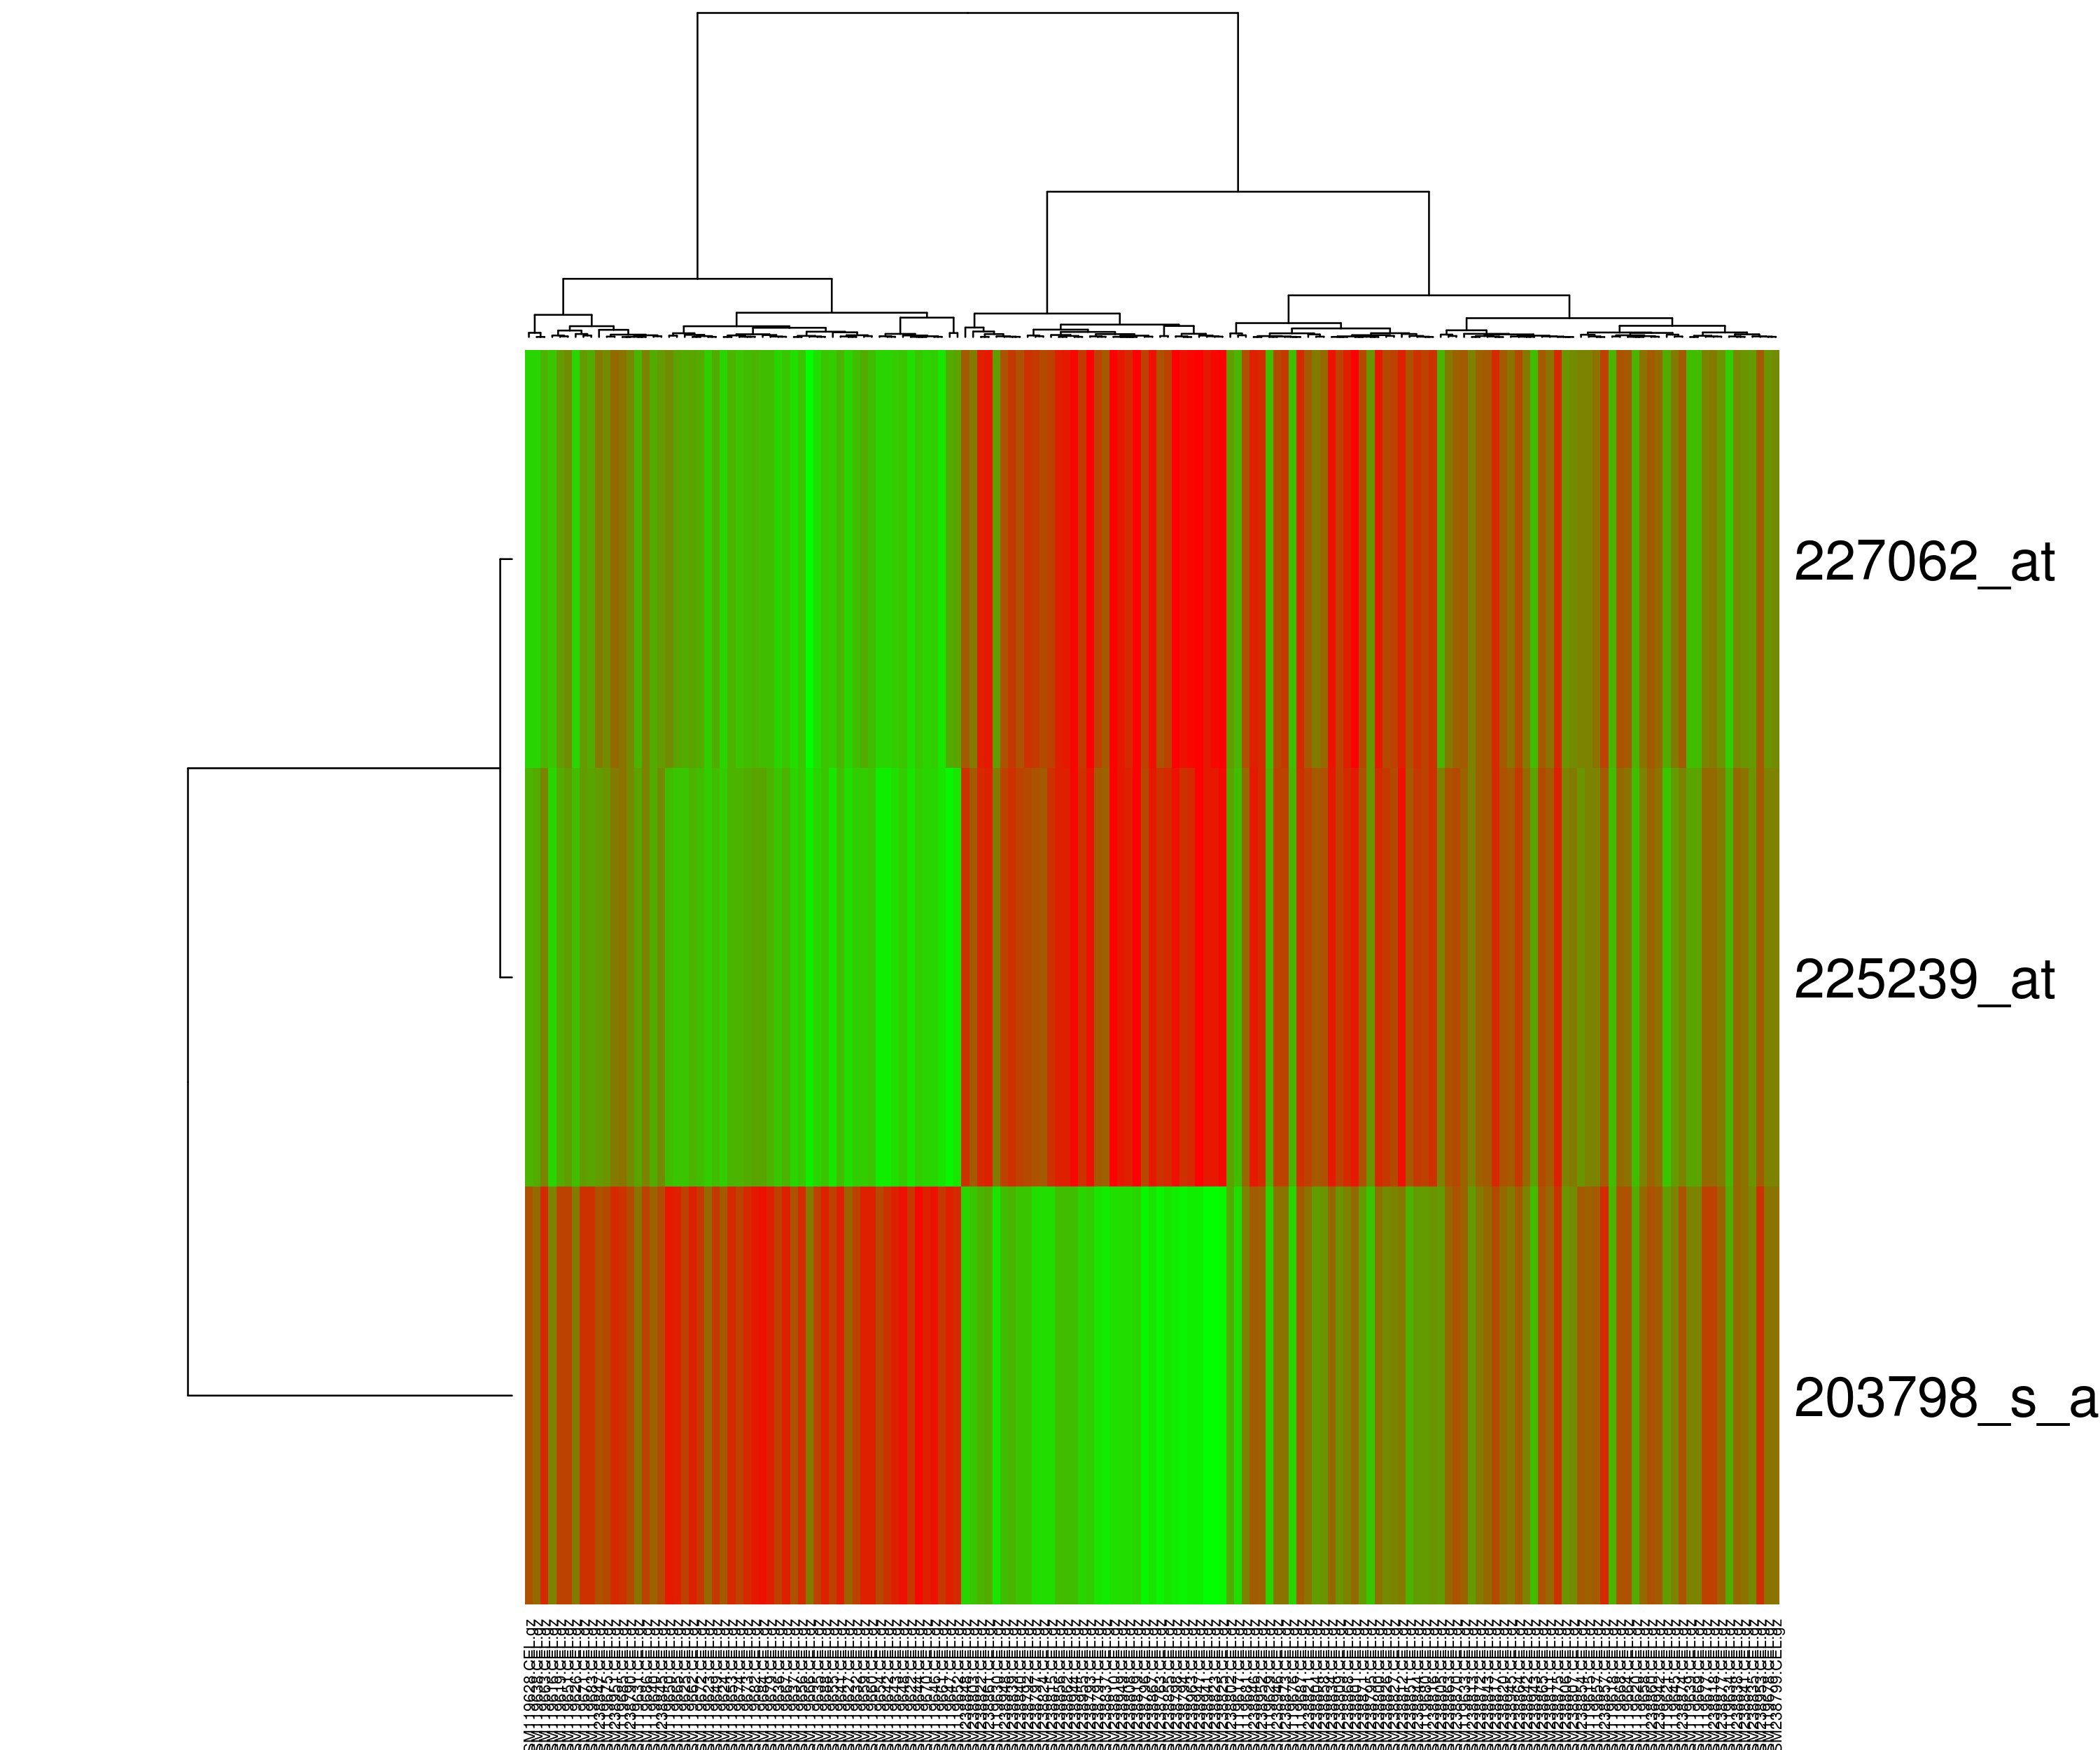
\includegraphics[width = .48\textwidth]{a_heatmap_s.png}}% 
    \caption{\texttt{Clusters from datasets obtained after filtering before statistical analysis}}
\end{figure}

\begin{figure}[h]
    \centering
    \subfloat[Statistically analysed data clustering]{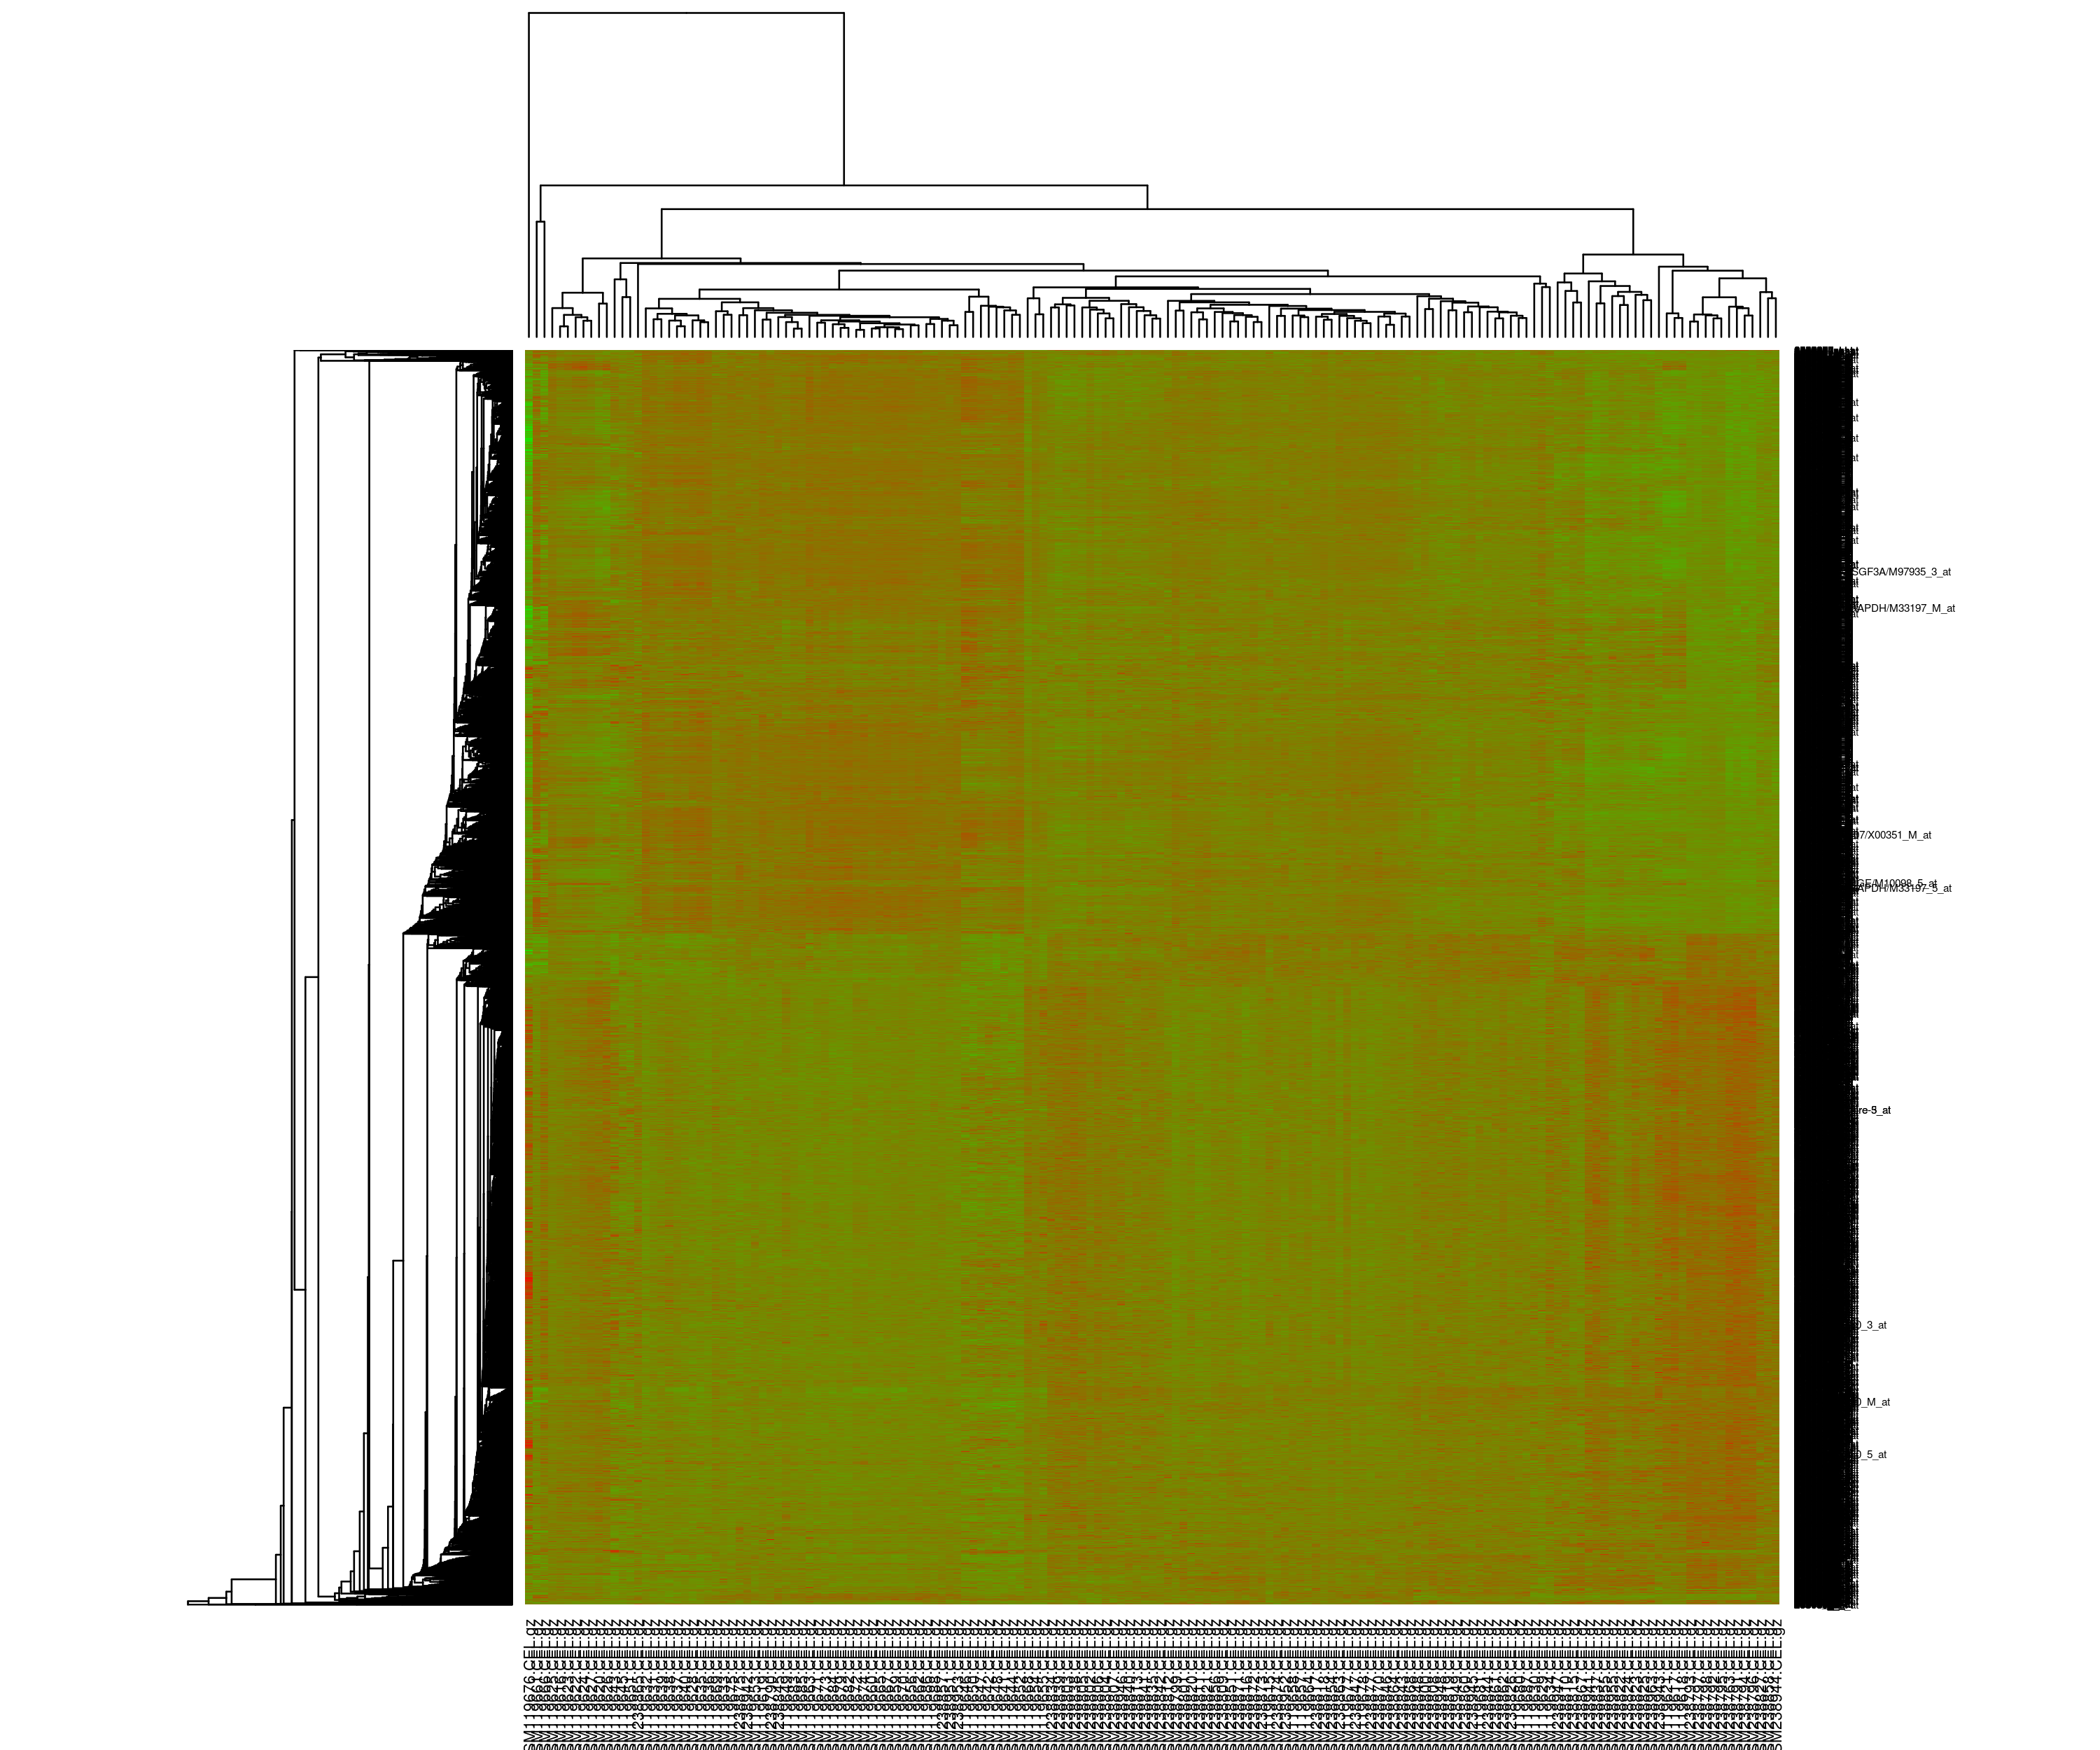
\includegraphics[width = \textwidth]{a_heatmap.png}}\hspace{1em}\\%
    \subfloat[Standard deviation filtered data clustering]{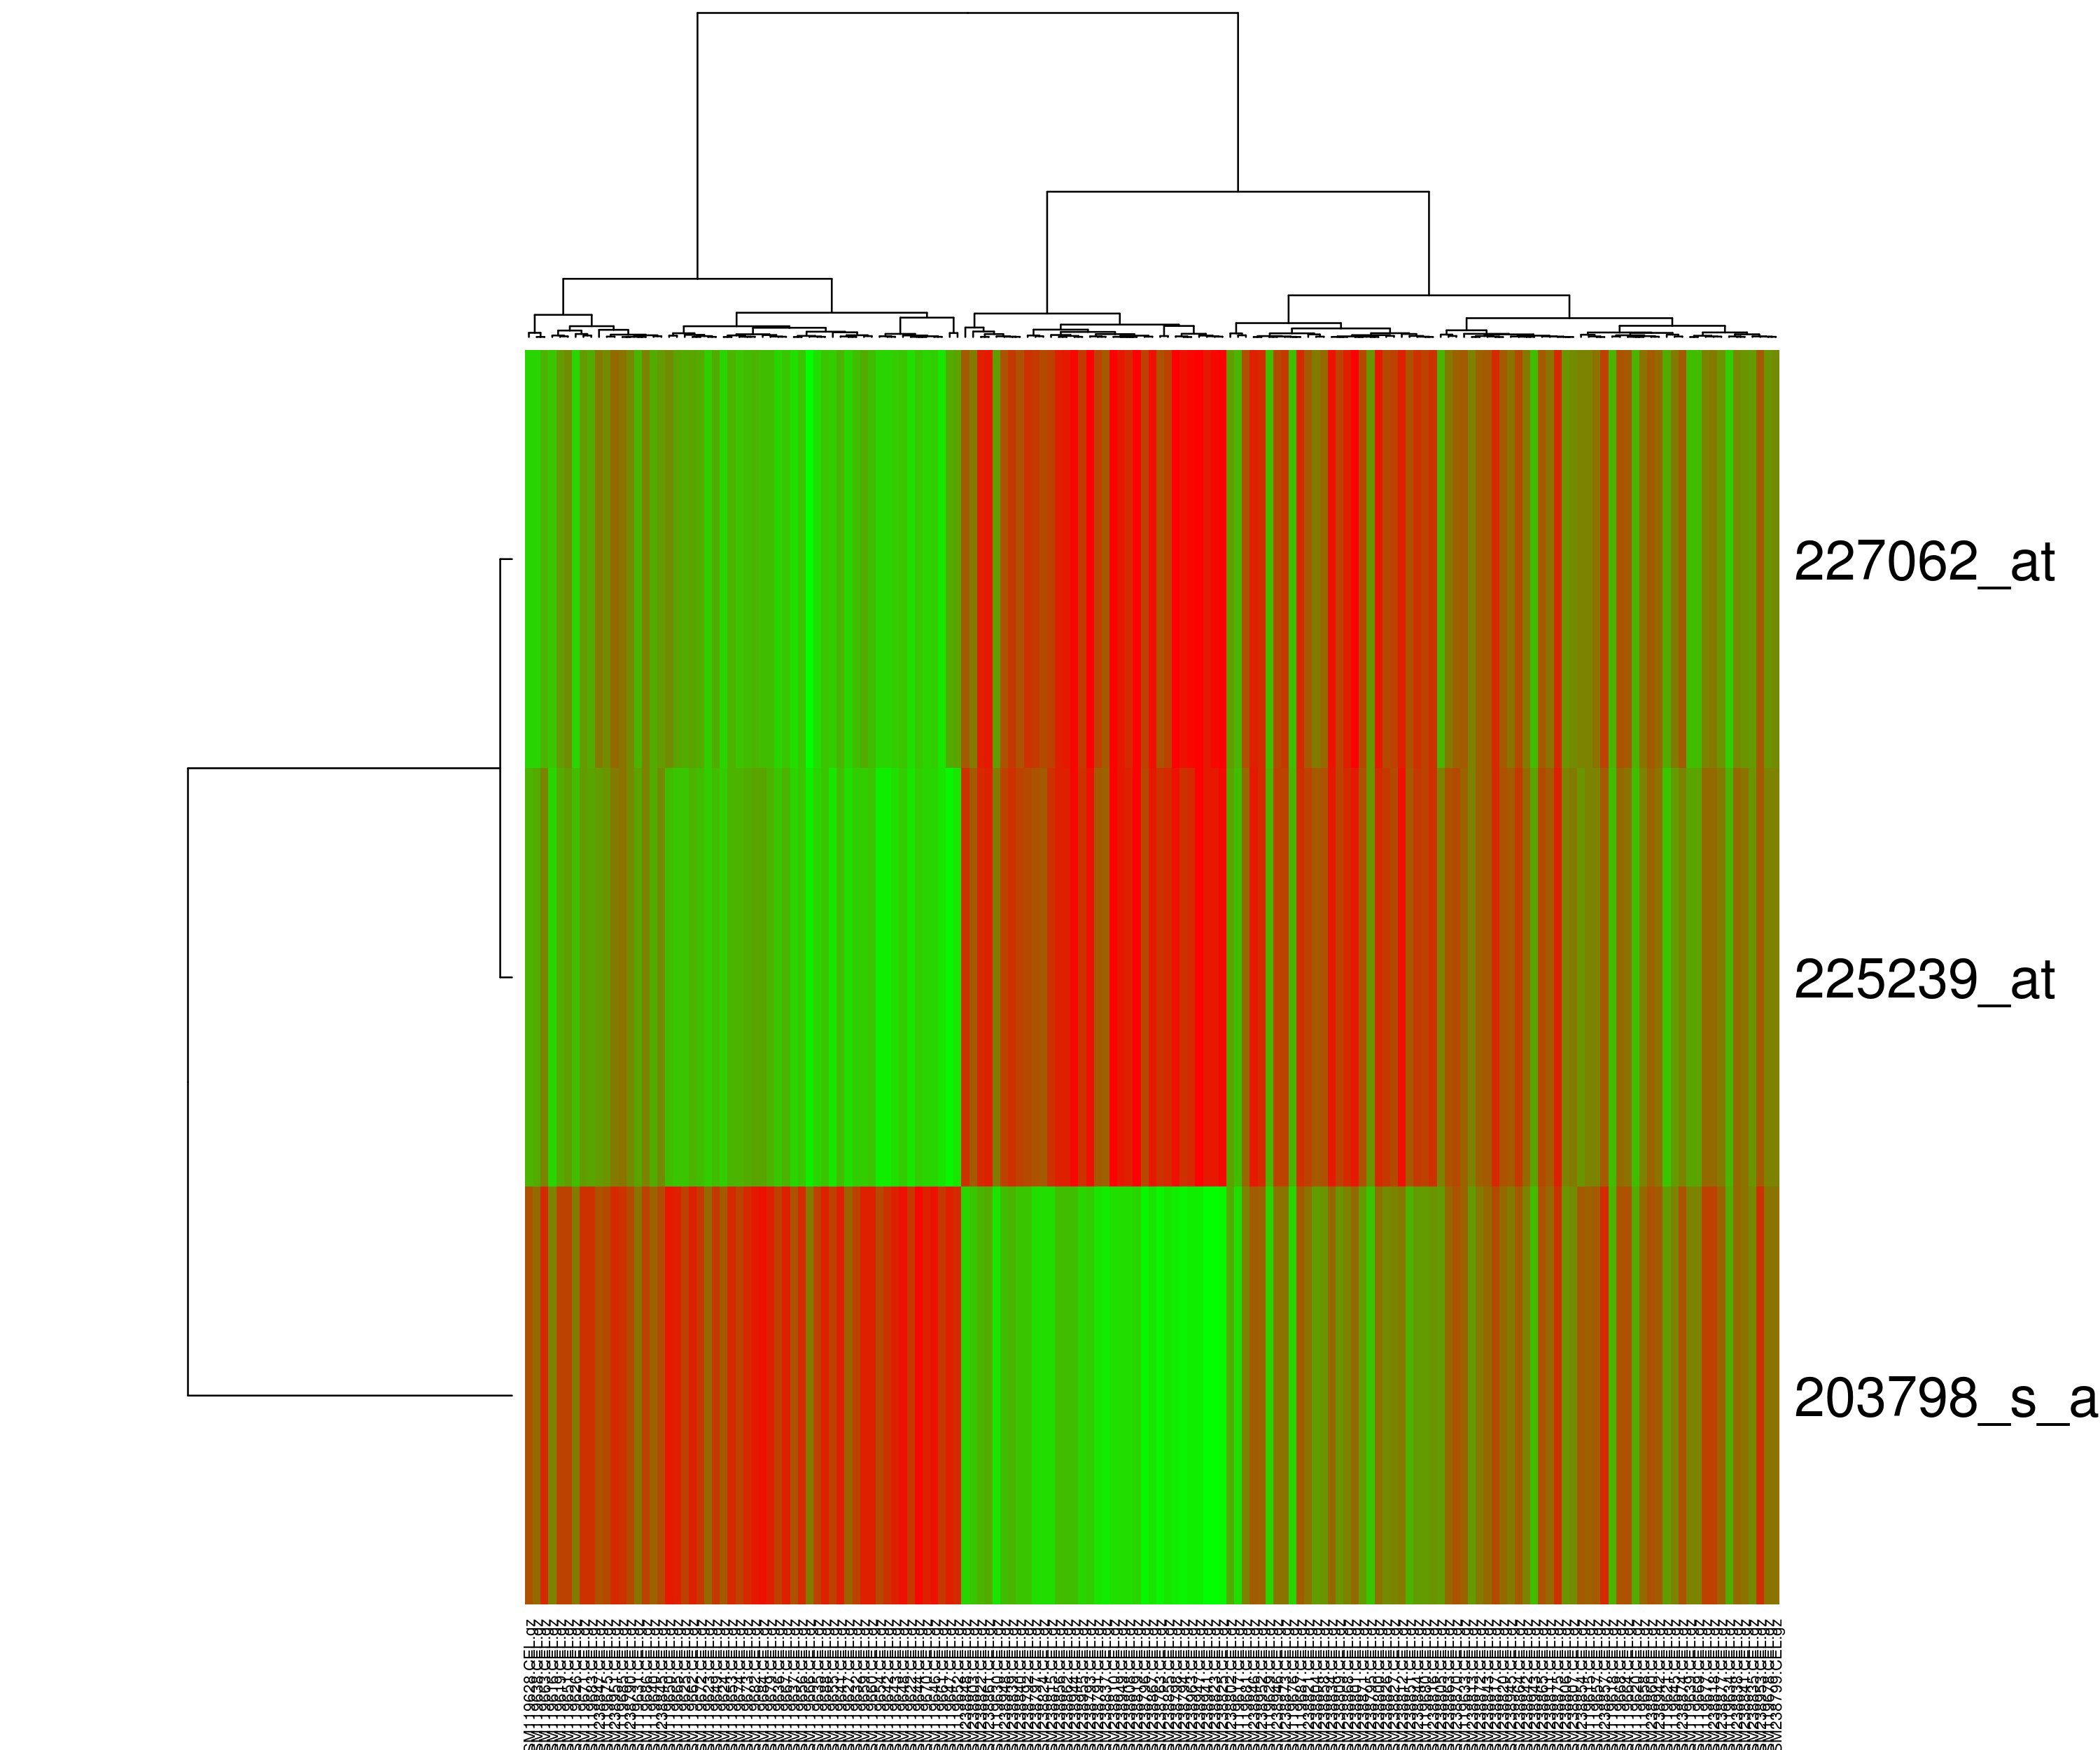
\includegraphics[width = .48\textwidth]{a_heatmap_s.png}}\hspace{1em}%
    \subfloat[Expression based filtered data clustering]{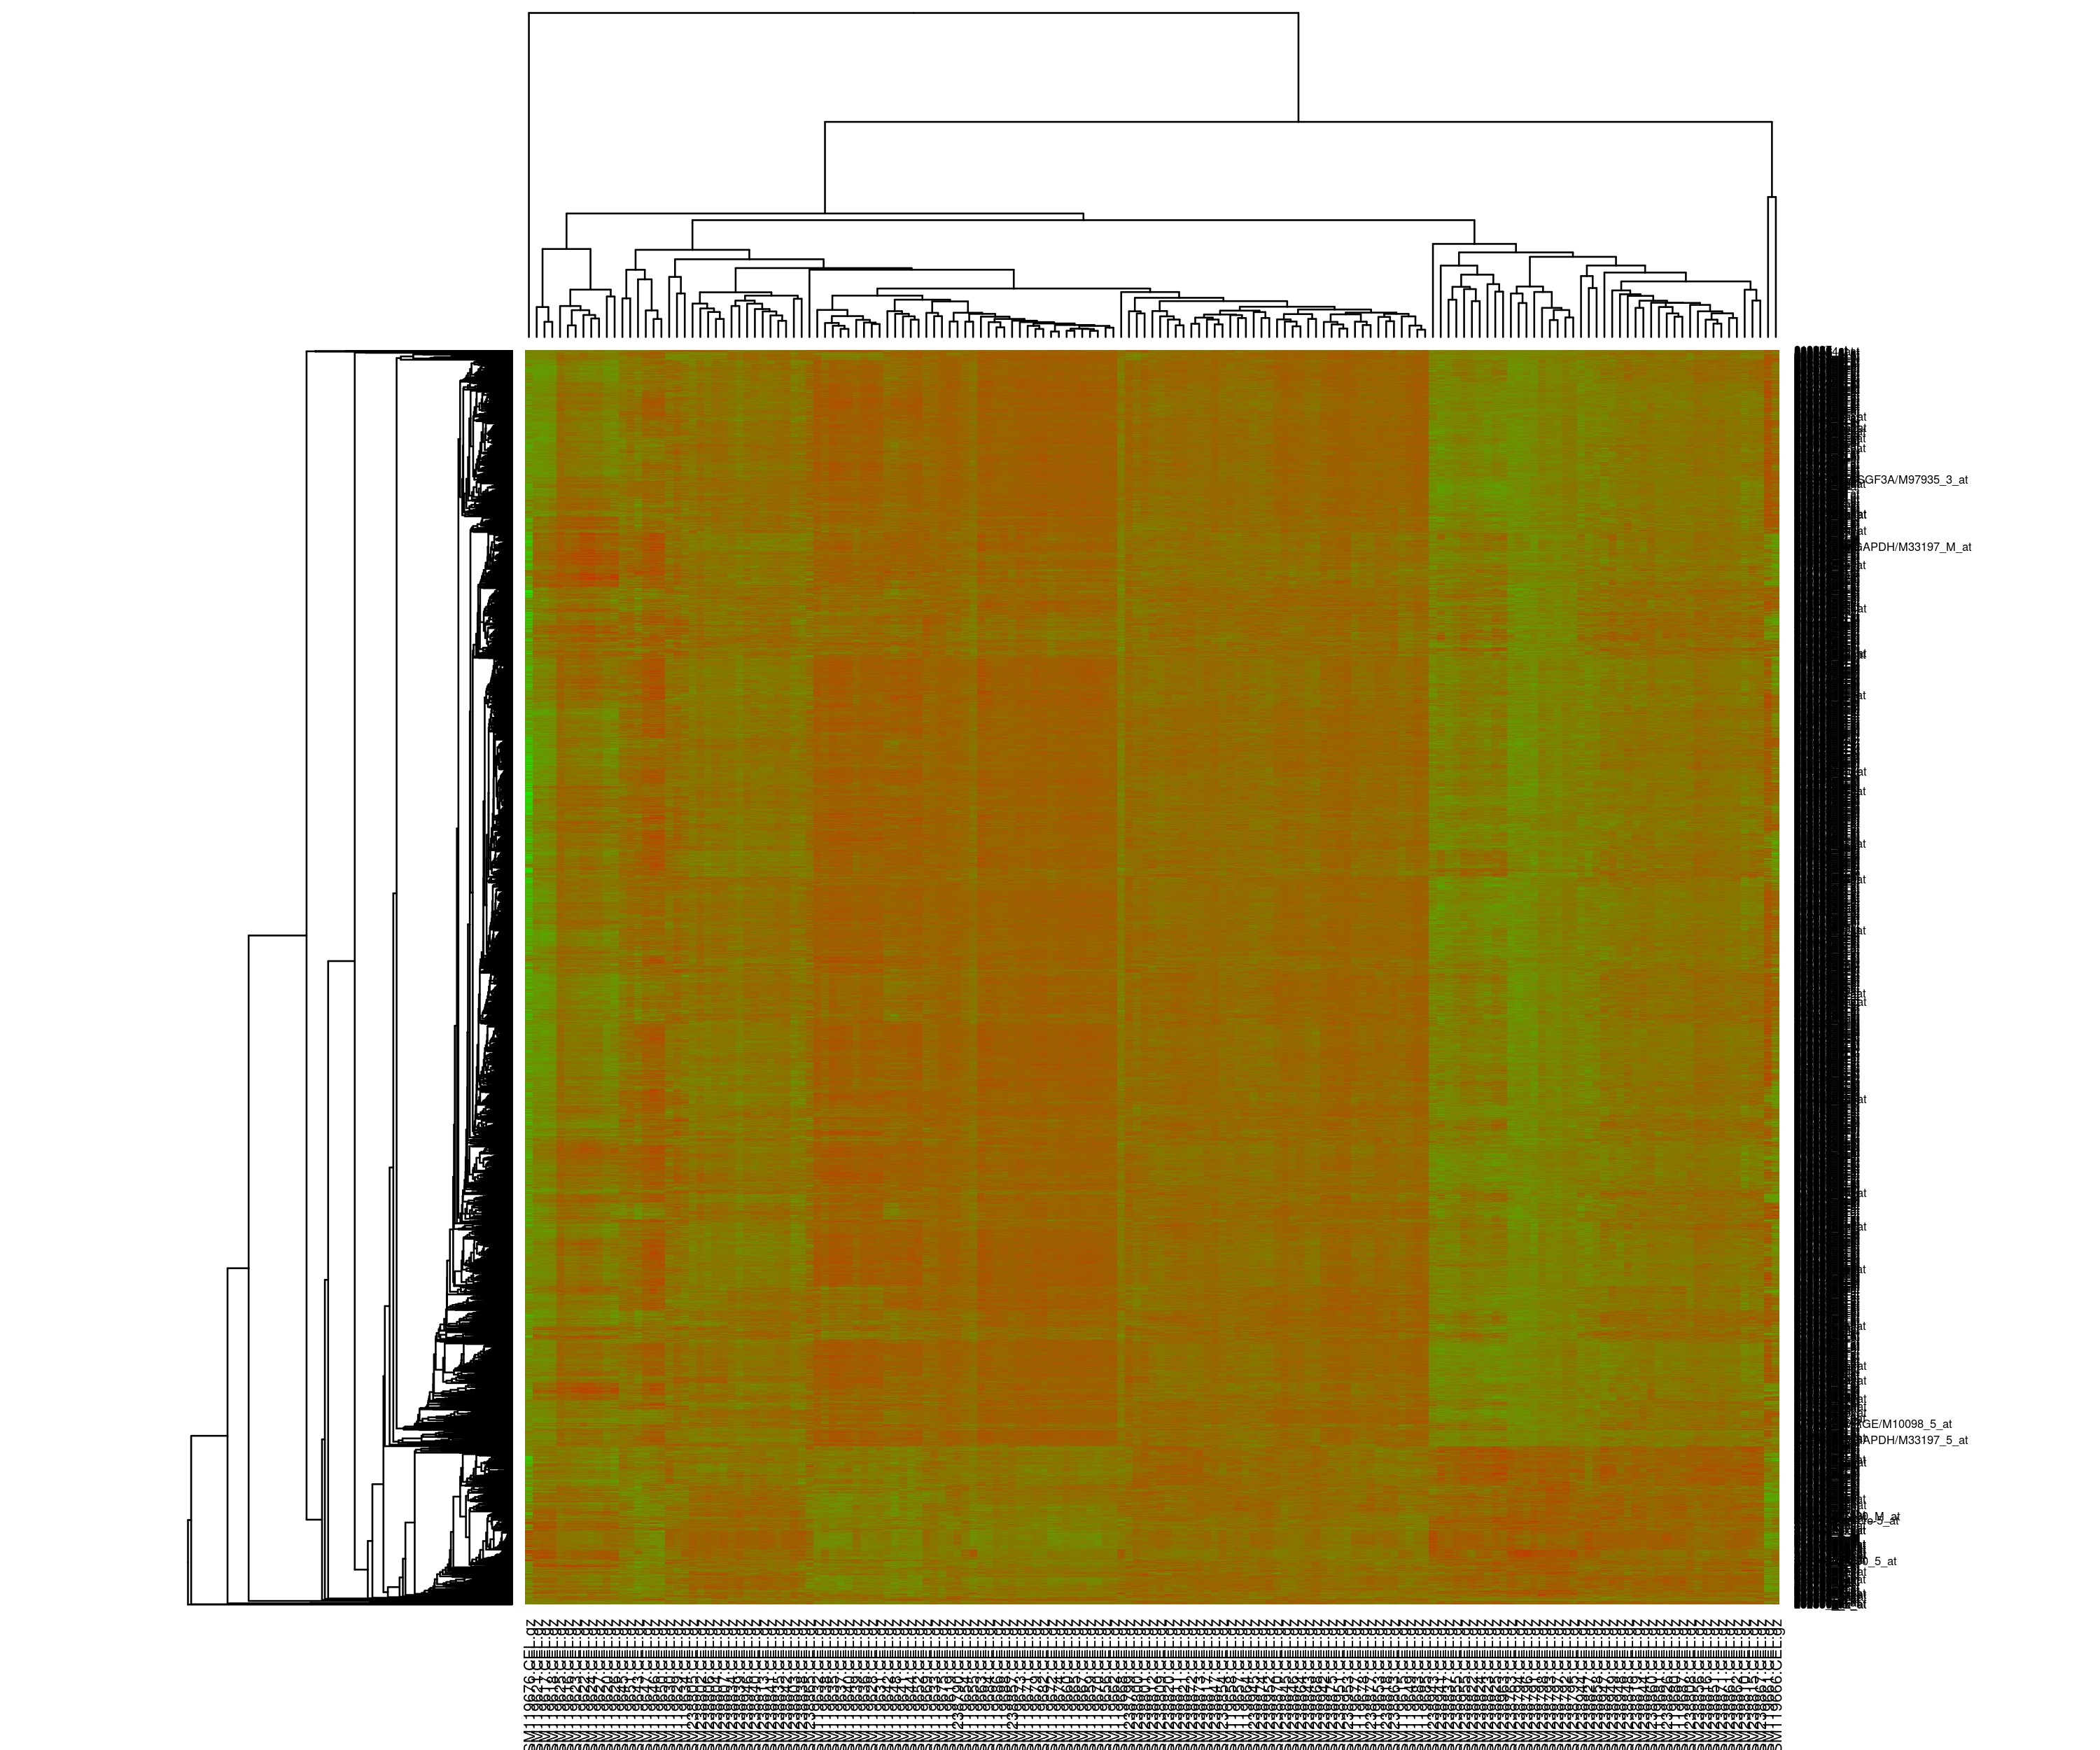
\includegraphics[width = .48\textwidth]{a_heatmap_e.png}}\hspace{1em}%
    \caption{\texttt{Clusters from datasets obtained after filtering after statistical analysis}}
\end{figure}

\subsection{k-Means Clustering}
Command \texttt{kmeans()} calculates a K-means clustering result. It takes four arguments - \texttt{x}, name of the data object; \texttt{centers}, number of clusters to create; \texttt{iter.max}, iteration maximum; \texttt{nstart}, which specifies how many times the run should be performed using the same settings. The analysis will be performed on \texttt{dat.s} or \texttt{dat.f}.

\begin{lstlisting}[language=R, caption=Performing k-means Clustering]
# Function kmeans() calculates a K-means clustering result.
# nstart specifies how many times the run should be performed
# using the same settings.

km <- kmeans(x=as.matrix(dat.m), centers=5, iter.max=100000, nstart=10)

sum(km$withinss)
# Output: [1] 3969607

head(km$cluster)
# Output:
# 1007_s_at   1053_at    117_at    121_at 1255_g_at   1294_at 
#         4         2         2         5         2         3

# Rows for which the km$cluster is equal to 1 can be extracted from the
# normalized data as follows
dat.c <- dat.m[km$cluster==1, ]
\end{lstlisting}

\subsection{Optimal number of clusters}
The analysis proceeds by changing the number of clusters, checking the results, and finally picking the solution that appears to be reasonable. Optimality of the solution can be checked using the within clusters sum of squares (within SS), and the idea is to minimize the within SS, but not to overfit the data, in other words, not to use too many clusters. Simply searching for the minimum WCSS is not a viable option, since it'll reach it’s minimum when the number of clusters is equal to the number of genes or arrays. Therefore, the K-means analysis is carried out using different numbers of clusters in each run. Then the number of clusters is plotted against within SS, and a point where the steep decent of the within SS starts to level off is the optimal number of clusters.

\begin{lstlisting}[language=R, caption=Optimal clusters]
optimal_clusters <- function(dat, fname){
    # Test a maximum of 100 clusters
    kmax <- c(30)
    
    # If there are less than 100 genes or arrays make the max.
    # no. of cluster equal to the number of genes or arrays.
    if(nrow(dat) < 30) {
        kmax <- nrow(dat)
    }
    
    # Create an empty vector for storing the within SS values
    km <- rep(NA, (kmax-1))
    # Minimum number of cluster is 2
    i <- c(2)
    # Test all numbers of clusters between 2 max. 100 using the while loop
    while(i < kmax) {
        km[i] <- sum(kmeans(dat.m, i, iter.max=20000, nstart=10)$withinss)
        # Terminate the run if the change in within SS is less than 1
    
        if(i >= 3 & km[i-1] / km[i] <= 1.99) {
            i <- kmax
        }else {
            i <- i + 1
        }
    }

    # Plot the number of K against the within SS
    png(paste(fname, "optimal.png"))
    plot(2:kmax, km, xlab="K", ylab="sum(withinss)", type="b", pch="+", main="Terminated when change less than 2%")
    dev.off()
}

# Clustering before the stat test
# Standard deviation filtered data
optimal_clusters(dat.f, "BeforeStatTest/StdFilter/f_")
# Statistically analysed, standard deviation filtered data
optimal_clusters(dat.s1, "BeforeStatTest/StdFilter/s_")
# Expression based filtered data
optimal_clusters(dat.fo, "BeforeStatTest/ExpFilter/f_")
# Statistically analysed, expression based filtered data
optimal_clusters(dat.s2, "BeforeStatTest/ExpFilter/s_")

# Analysis after the stat test.
# Statistically analysed data
optimal_clusters(dat.s, "AfterStatTest/")
# Statistically analysed, standard deviation filtered data
optimal_clusters(dat.s.f, "AfterStatTest/StdFilter/")
# Statistically analysed, expression based filtered data
optimal_clusters(dat.s.fo, "AfterStatTest/ExpFilter/")
\end{lstlisting}

\begin{figure}[h]
    \centering
    \subfloat[Standard deviation filtered data, optimal no. of clusters are 4]{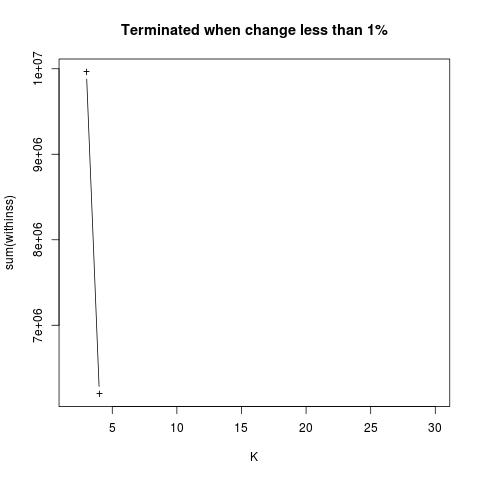
\includegraphics[width = .48\textwidth]{bf_optimal.png}}\hspace{1em}%
    \subfloat[Statistically analysed, standard deviation data, optimal no. of clusters which is shown in the plot is 3, but in this dataset there are 3 genes only. Thus, no 2 genes show similar properties to belong to a single cluster. Hence, clustering this dataset won't be helpful.]{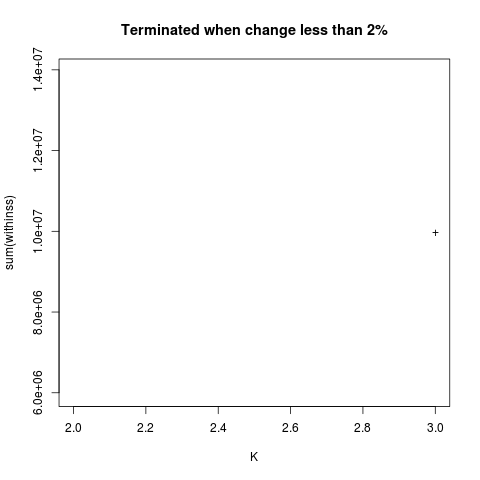
\includegraphics[width = .48\textwidth]{bs_optimal.png}}\hspace{1em}\\%
    \subfloat[Expression based filtered data, optimal no. of clusters are 4]{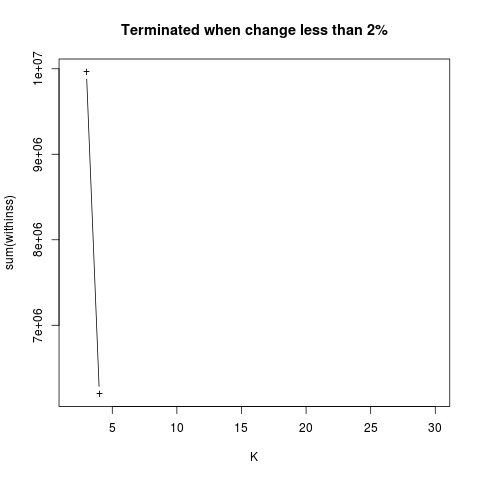
\includegraphics[width = .48\textwidth]{af_optimal.png}}\hspace{1em}%
    \subfloat[Statistically analysed, expression based filtered data, optimal no. of clusters are 4]{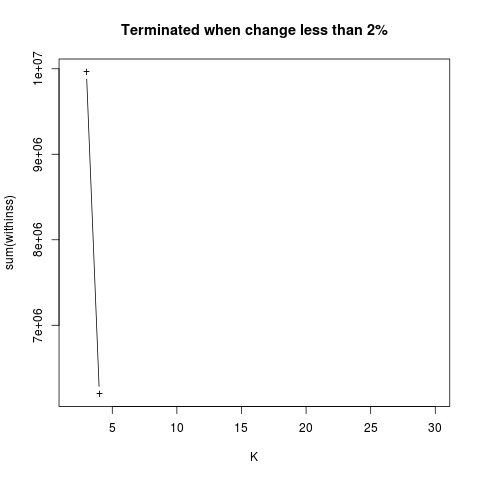
\includegraphics[width = .48\textwidth]{as_optimal.png}}% 
    \caption{\texttt{Optimal clusters plot}, from datasets obtained after filtering before statistical analysis}
\end{figure}

\begin{figure}[h]
    \centering
    \subfloat[Statistically analysed data, optimal no. of clusters are 4]{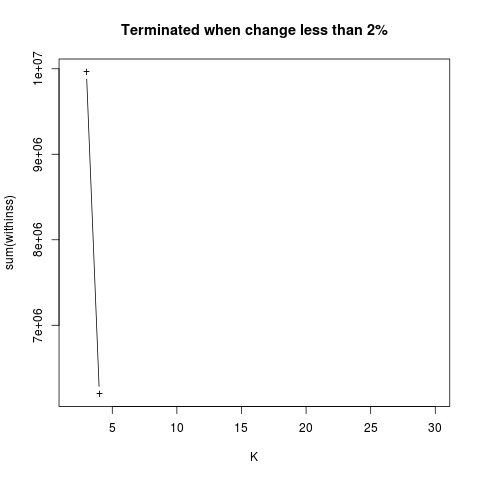
\includegraphics[width = .30\textwidth]{optimal.png}}\hspace{1em}%
    \subfloat[Statistically analysed, standard deviation data, optimal no. of clusters, which is shown in the plot is 3, but in this dataset there are 3 genes only. Thus, no 2 genes show similar properties to belong to a single cluster. Hence, clustering this dataset won't be helpful.]{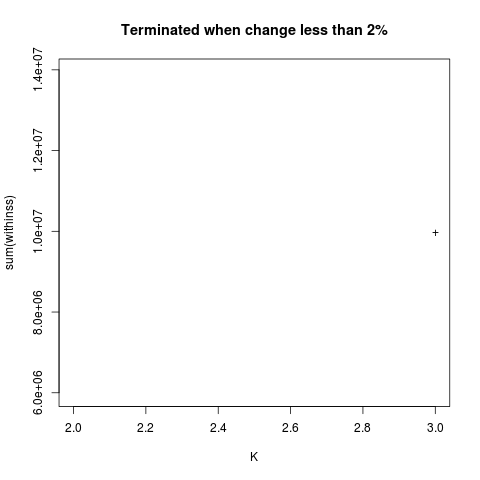
\includegraphics[width = .30\textwidth]{optimal_s.png}}\hspace{1em}%
    \subfloat[Statistically analysed, expression based filtered data, optimal no. of clusters are 4]{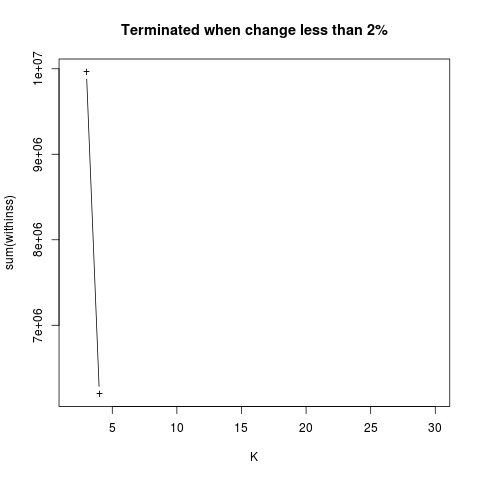
\includegraphics[width = .30\textwidth]{optimal_e.png}}% 
    \caption{\texttt{Optimal clusters plot}, from datasets obtained after filtering after statistical analysis}
\end{figure}

\subsection{Visualizing}
K-means clustering is usually visualized by drawing the gene expression pattern across the arrays using a single line graph per cluster. Command \texttt{matplot()} does the actual plotting. Every single gene is represented by one line in the plot.

\begin{lstlisting}[language=R, caption=k-means Clustering]
clustering <- function(dat, clusters, fname){
    km <- kmeans(x=as.matrix(dat), algorithm="Lloyd",
    centers=clusters, iter.max=200000, nstart=10)
    
    # K-means clustering is usually visualized by drawing the gene expression
    # pattern across the arrays using a single line graph per cluster.
    # Function matplot() does the actual plotting.
    # The idea is to get a general view of the pattern in the data.
    
    max.dat <- max(dat)
    min.dat <- min(dat)
    
    k <- c(clusters)

    # Plot the number of K against the within SS
    png(paste(fname, "kmeans.png"), width=12, height=7, units="in", res=250)
    par(mfrow=c(ceiling(sqrt(k)), ceiling(sqrt(k))))
    
    for(i in 1:k) {
        matplot(t(dat[km$cluster==i,]), type="l",
        main=paste("cluster:", i), ylab="log expression",
        col=1, lty=1, ylim=c(min.dat, max.dat))
    }
    dev.off()
}

# Clustering before the stat test
# Standard deviation filtered data
clustering(dat.f, 4, "BeforeStatTest/StdFilter/f_")
# Expression based filtered data
clustering(dat.fo, 4, "BeforeStatTest/ExpFilter/f_")
# Statistically analysed, expression based filtered data
clustering(dat.s2, 4, "BeforeStatTest/ExpFilter/s_")

# Analysis after the stat test.
# Statistically analysed data
clustering(dat.s, 4, "AfterStatTest/")
# Statistically analysed, expression based filtered data
clustering(dat.s.fo, 4, "AfterStatTest/ExpFilter/")
\end{lstlisting}

\begin{figure}
    \centering
    \subfloat[\texttt{k-means clustering}, standard deviation filtered data clustering]{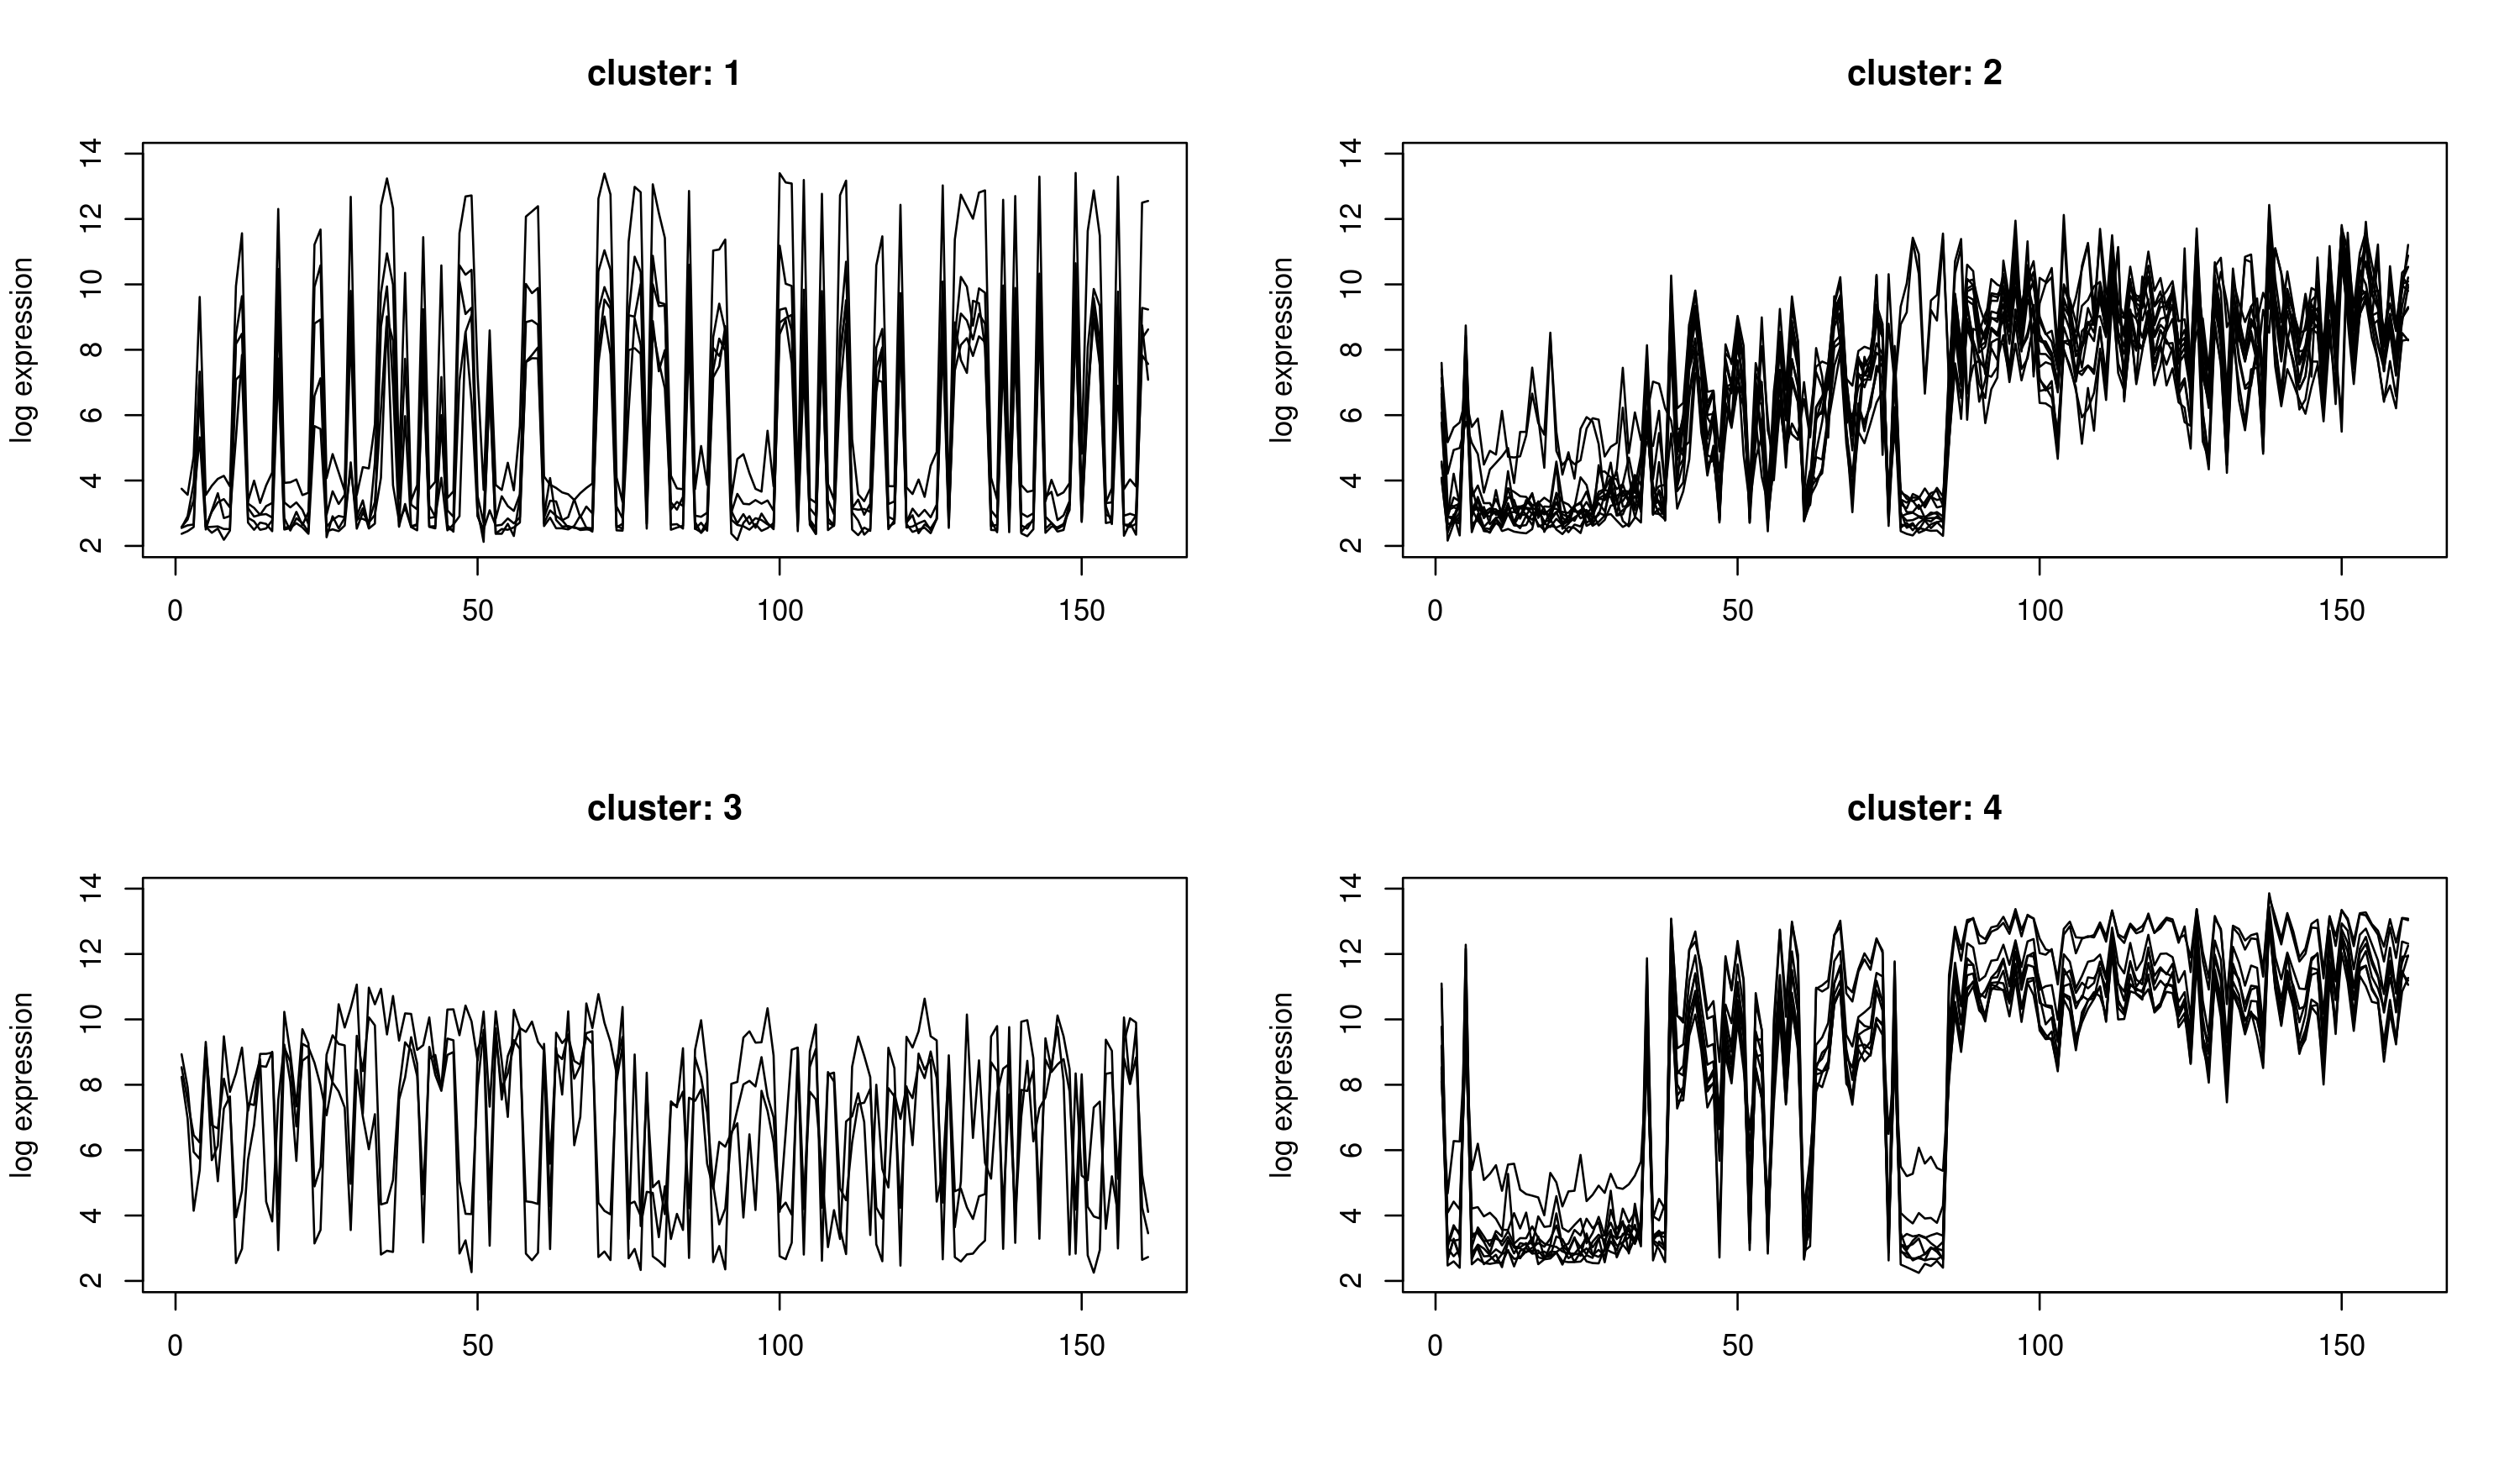
\includegraphics[width = \textwidth]{bf_kmeans.png}}\\%
\end{figure}

\begin{figure}
    \centering
    \ContinuedFloat
    \subfloat[\texttt{k-means clustering}, expression based filtered data]{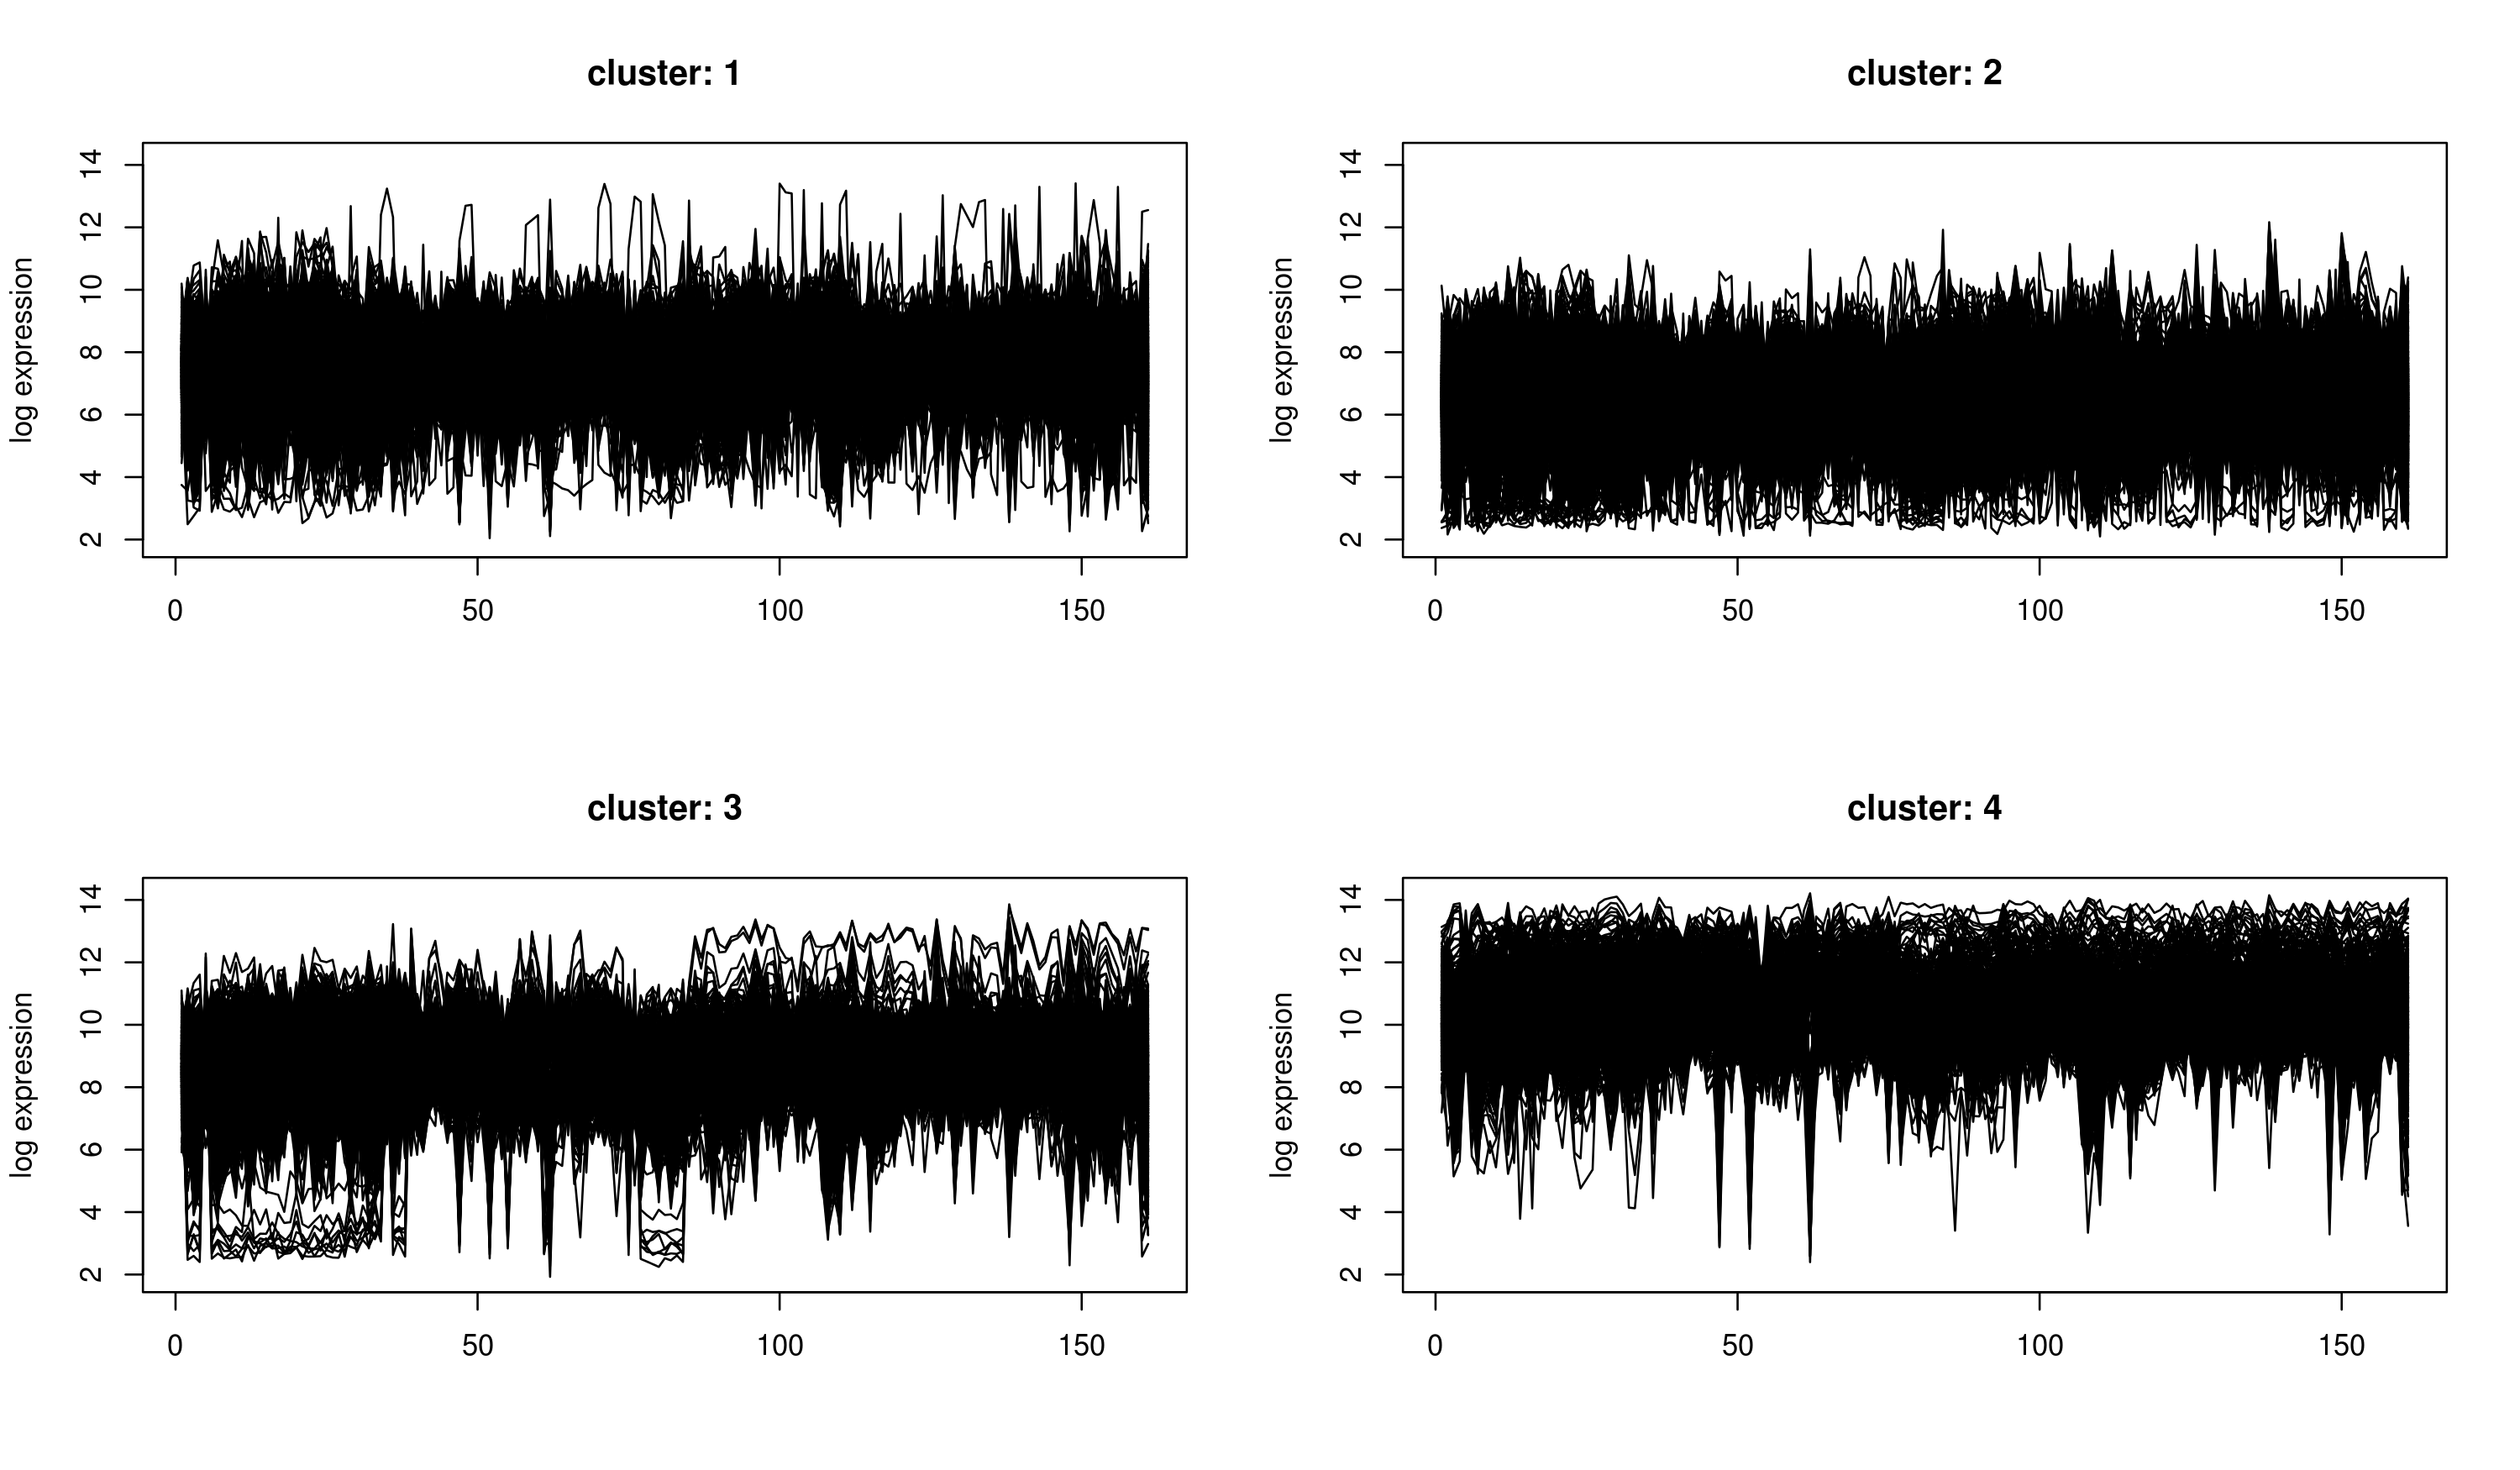
\includegraphics[width = \textwidth]{af_kmeans.png}}\\%
    \subfloat[\texttt{k-means clustering}, statistically analysed, expression based filtered data]{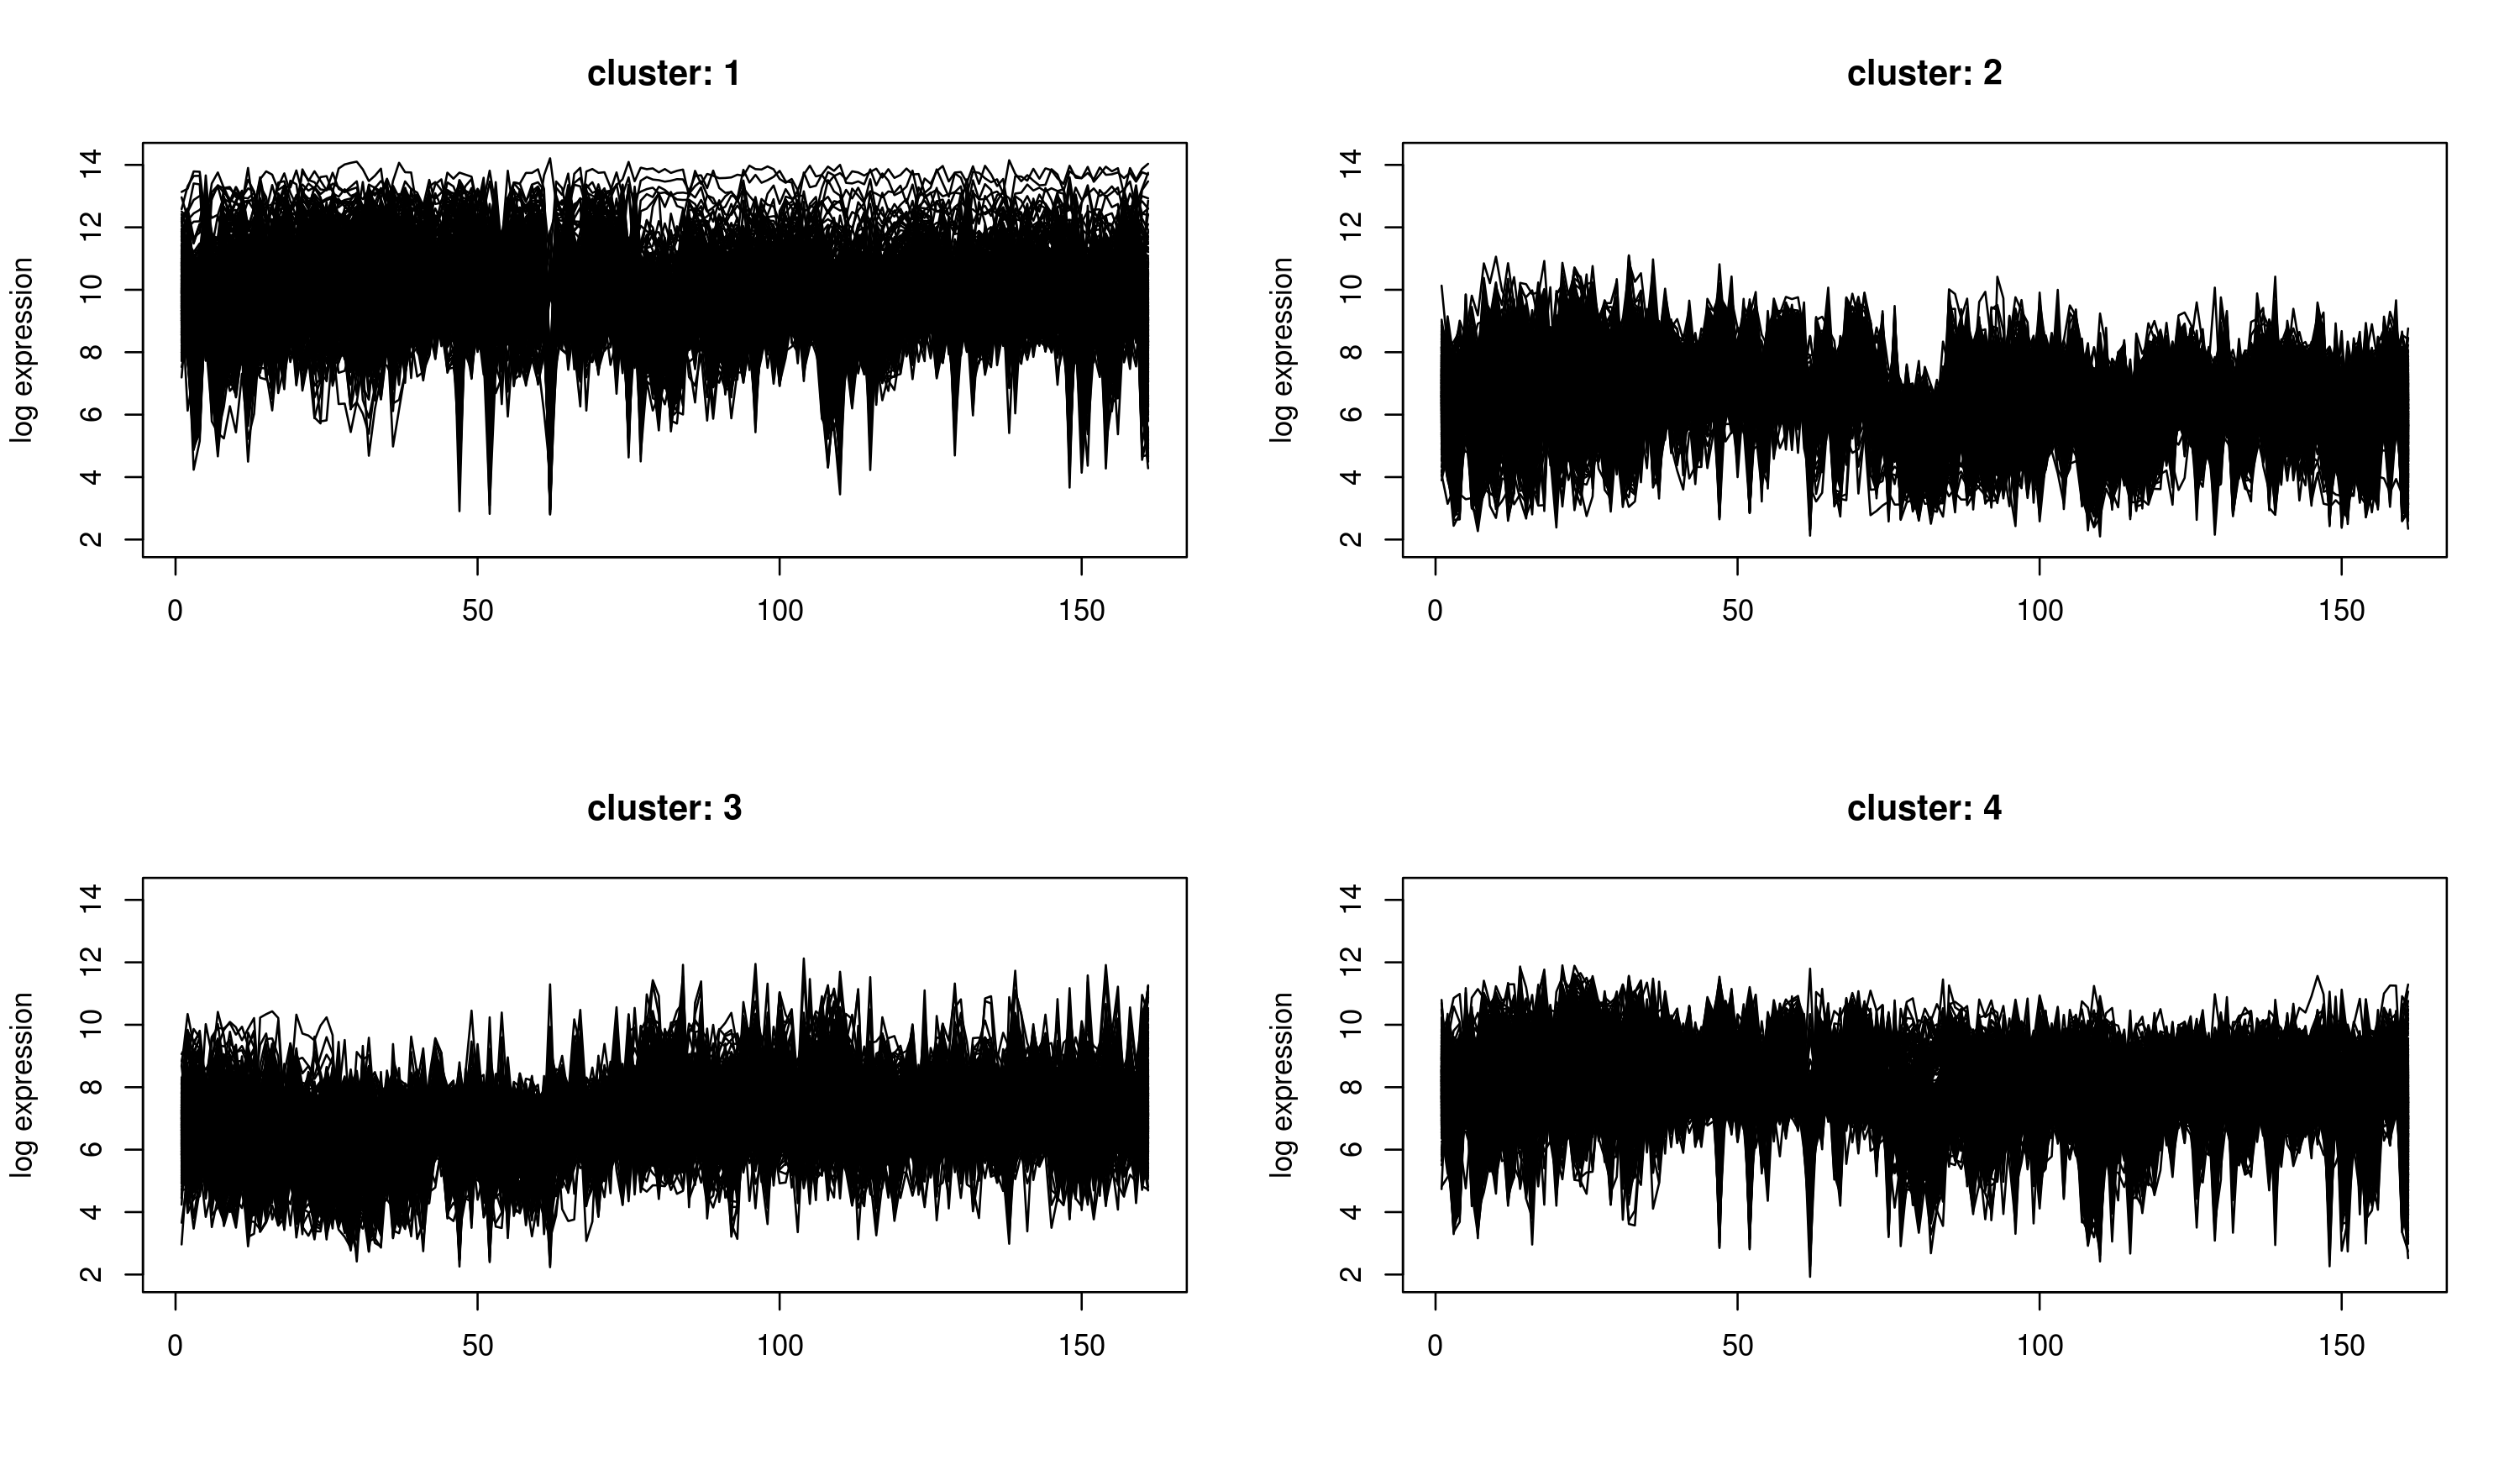
\includegraphics[width = \textwidth]{as_kmeans.png}}%
    \caption{\texttt{k-means clustering}, for data obtained after doing statistical analysis on the filtered data}
\end{figure}

\begin{figure}
    \centering
    \subfloat[\texttt{k-means clustering}, statistically analysed data]{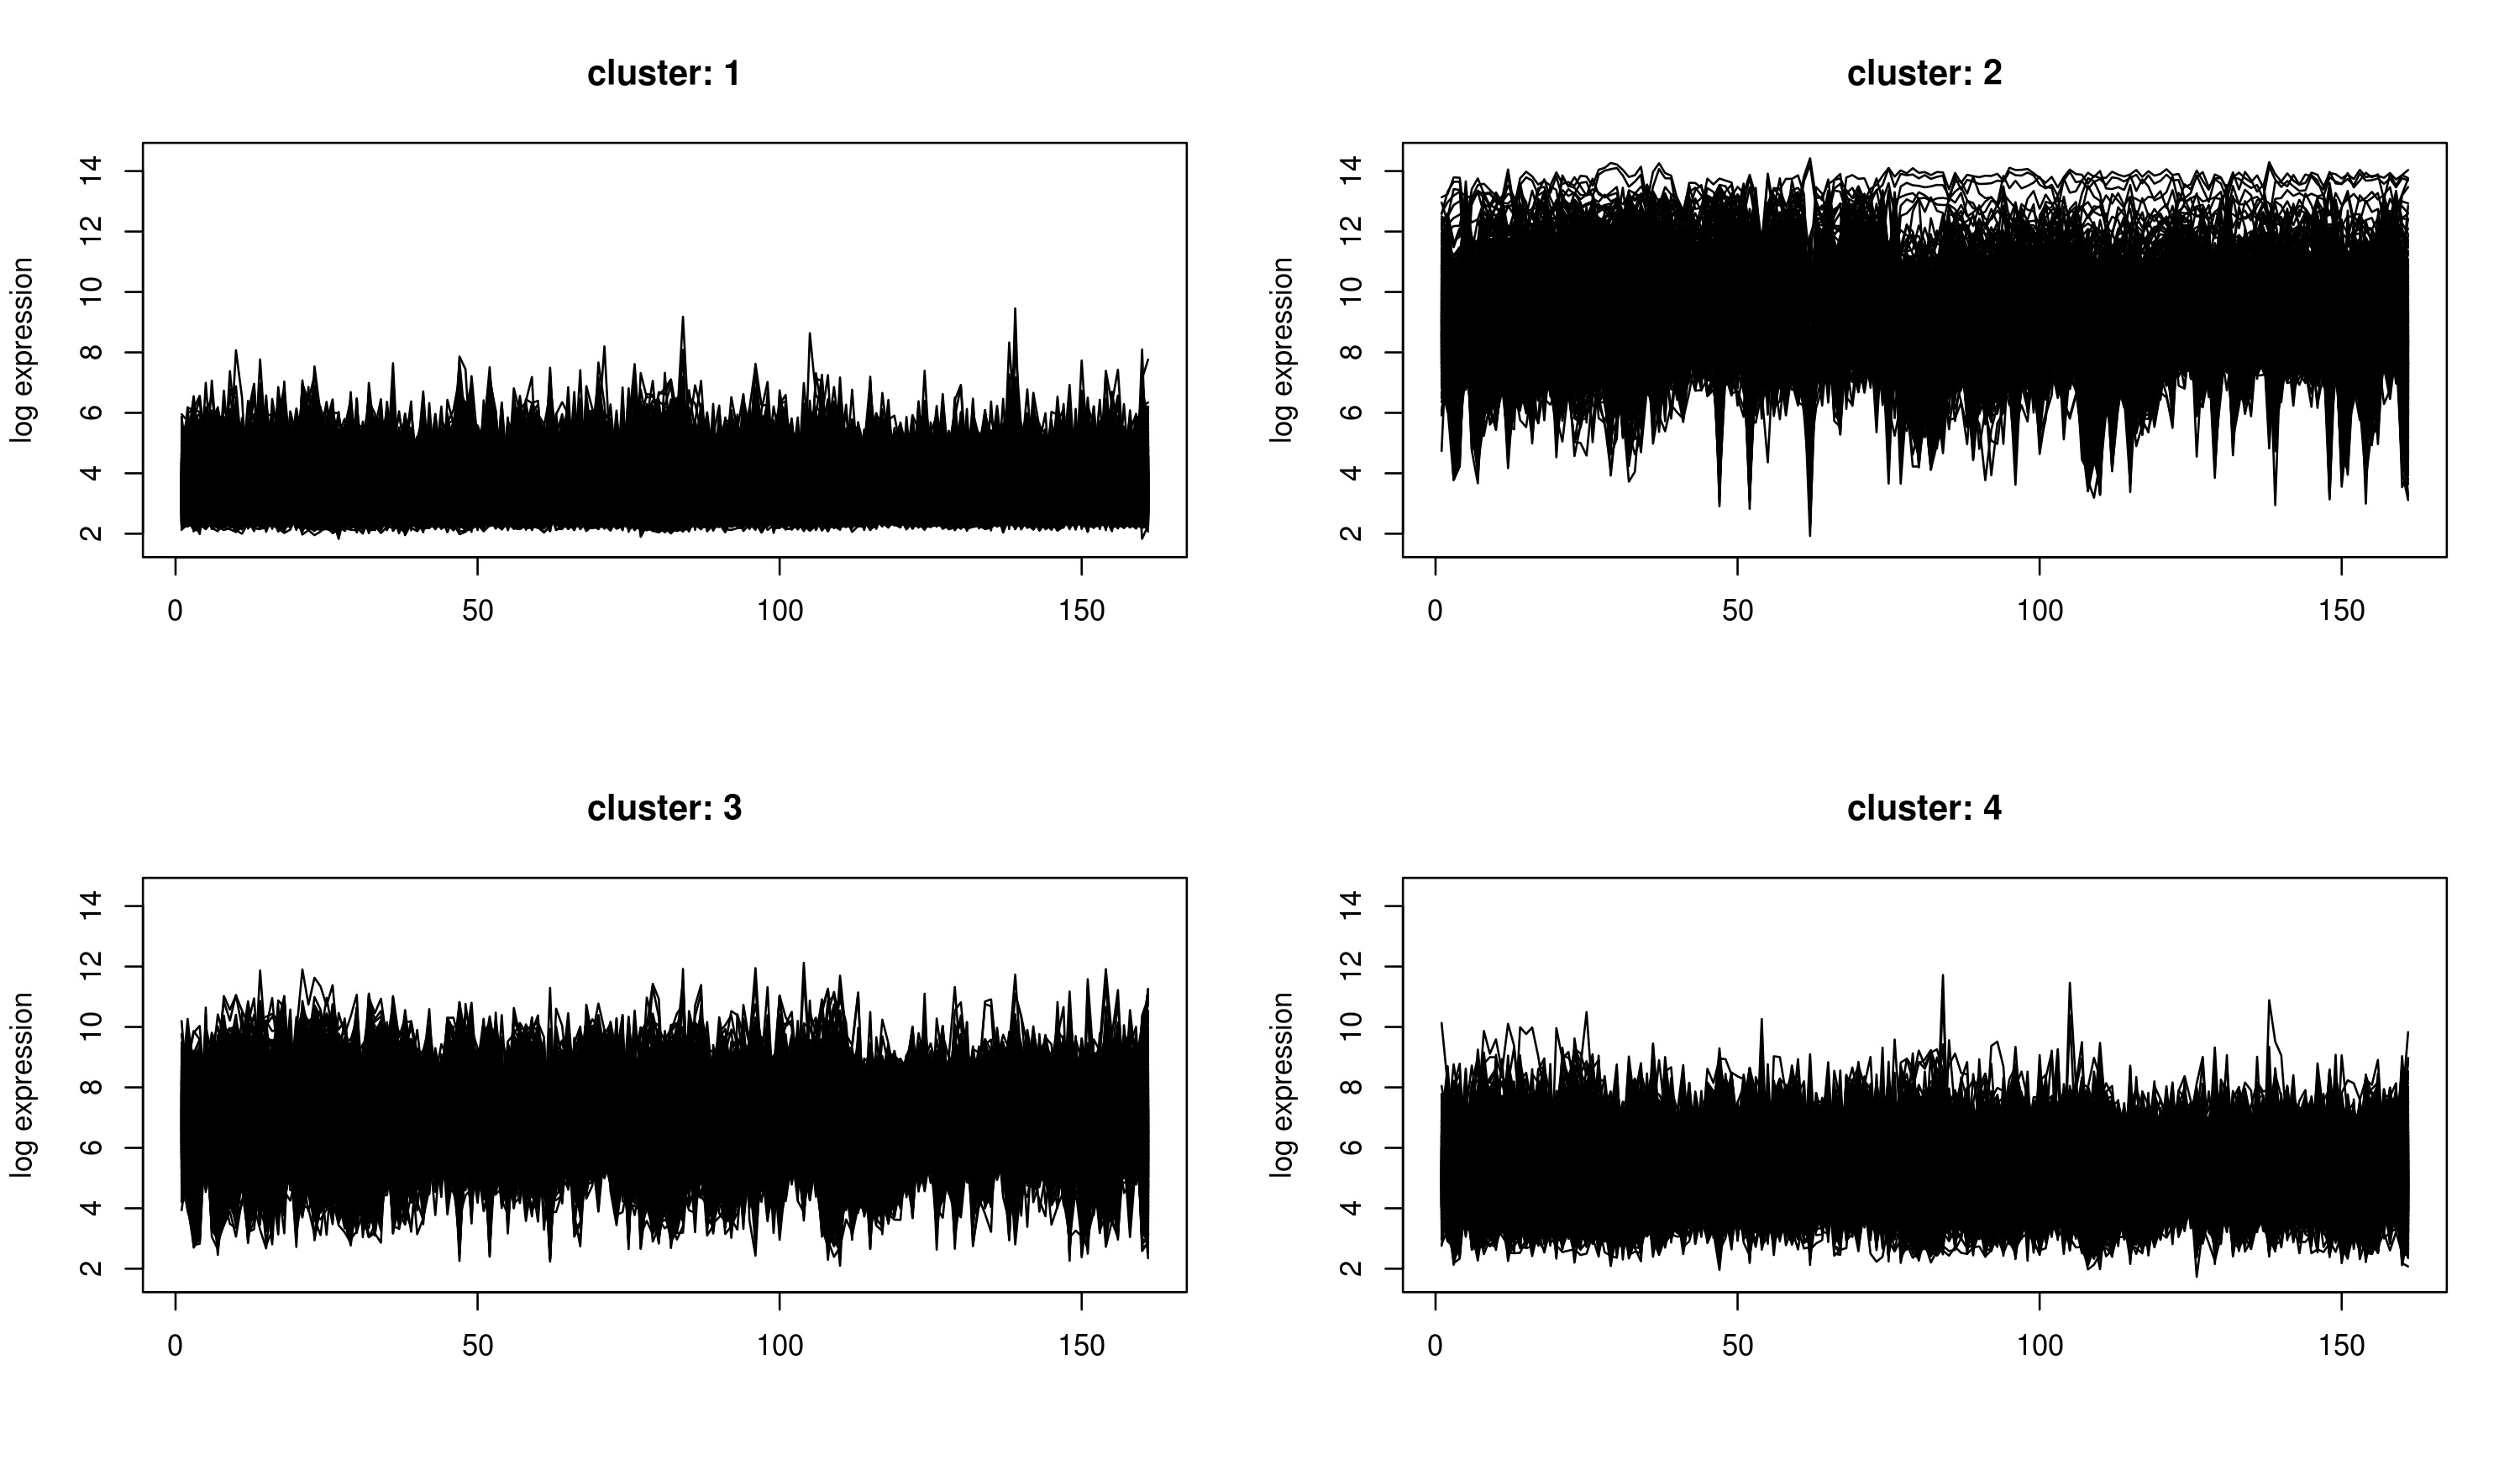
\includegraphics[width = \textwidth]{a_kmeans.png}}\\%
    \subfloat[\texttt{k-means clustering}, expression based filtered data]{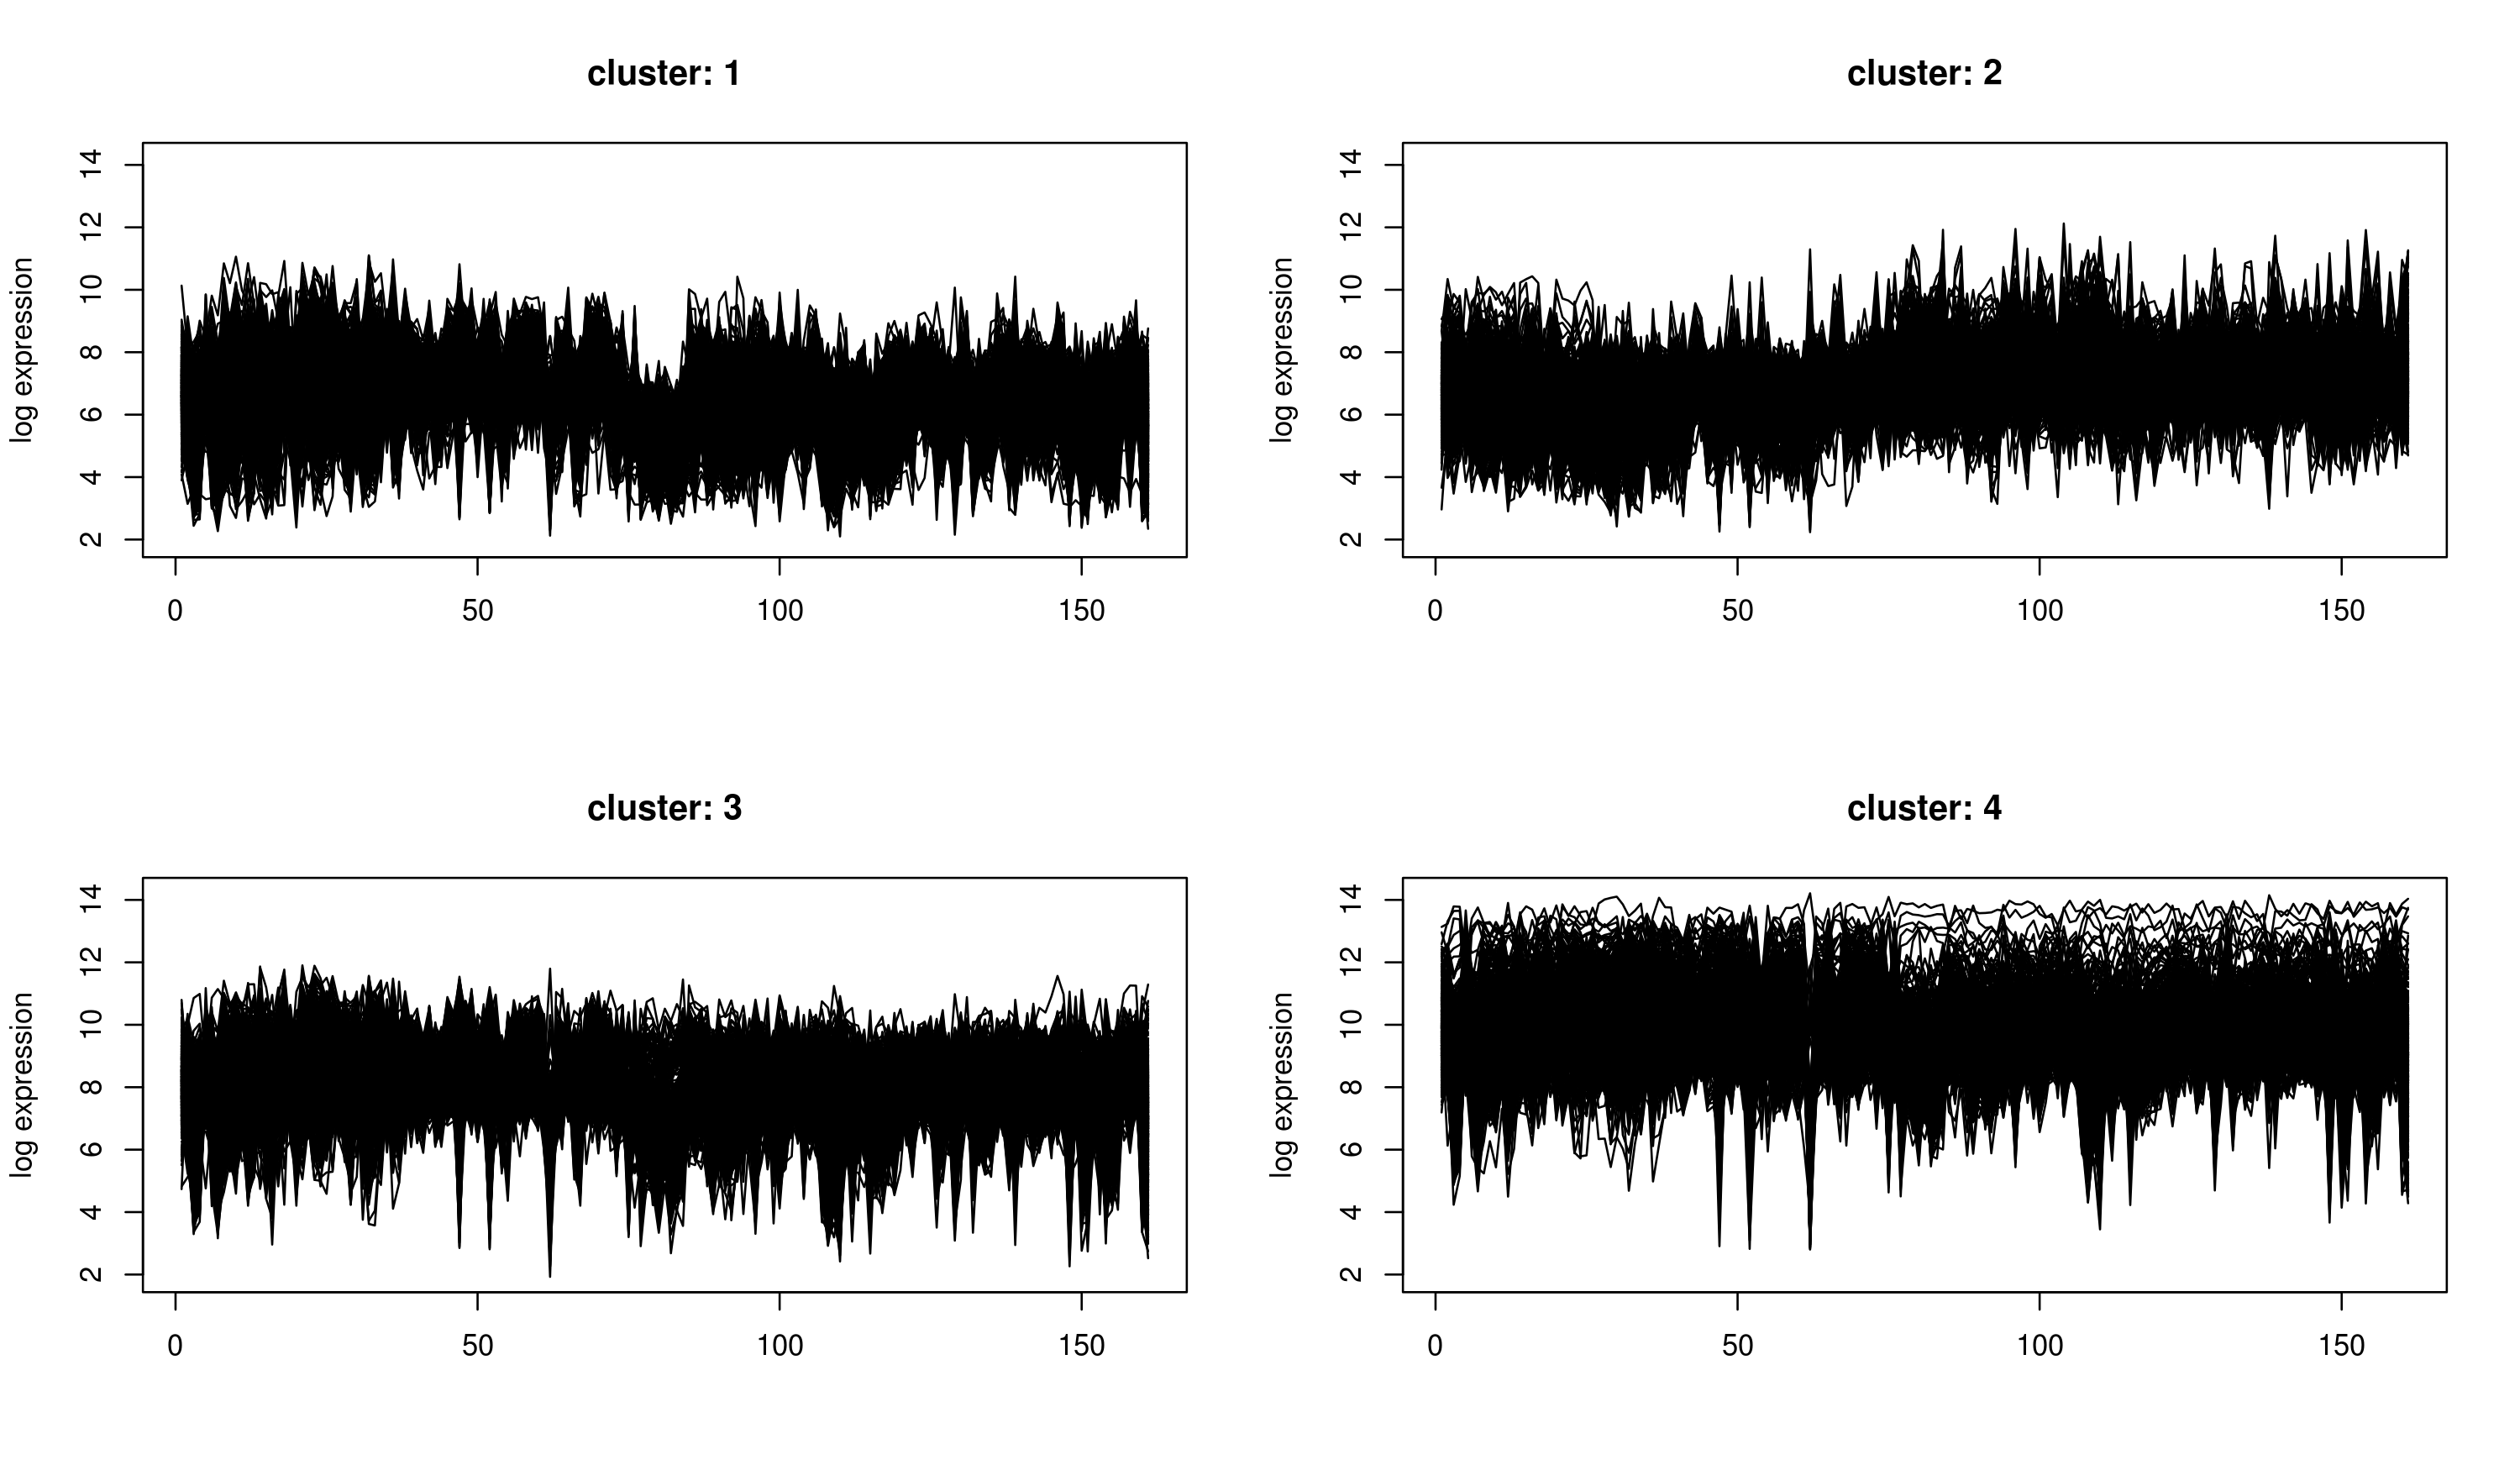
\includegraphics[width = \textwidth]{kmeans_e.png}}%
    \caption{\texttt{k-means clustering}, for data obtained after doing statistical analysis before the filtering}
\end{figure}


%%%%%%%%%%%%%%%%%%%
%%%%% RESULTS %%%%%
%%%%%%%%%%%%%%%%%%%
\chapter{Results}
\markboth{}{}
Thus, in this study I learned the basic of microarray data analysis. I loaded the data using R in a Linux environment. Then pre-processed it using normalization and filtering techniques. Pre-processing was followed by the statistical analyses, namely, getting differentially expressed genes using linear model and gene set enrichment analysis. The expressed genes extracted in the previous step were clustered and visualized.

During this whole process I skipped over some details and processes to get to the objective. Hence, a lot of work remains to be done to do this study satisfactorily, but I covered some of the major ground in this study and learned various aspects of computational biology and computer science as well.


%%%%%%%%%%%%%%%%%%%%%%%%%%%%%%%%%%%%%%%
%%%%% CONCLUSIONS AND FUTURE WORK %%%%%
%%%%%%%%%%%%%%%%%%%%%%%%%%%%%%%%%%%%%%%
\chapter{Conclusions and Future Work}
\markboth{}{}
This was the initial part of the study. Just getting to know the basic steps of the microarray data analysis. Now, there are many directions in which we can move after this. Or may be, keeping the same objective and modelling a GRN by opting one of various computational tools.

\section{Mutual Information}
This is a pre-processing step for the modelling of GRNs. By systematically analyzing the mutual information (governed by Shannon's entropy) between input states and output states, one is able to infer the sets of input elements controlling each element or gene in the network\cite{liang, wang, adam}. This technique gives us which genes may regulate a particular gene, but it doesn't tell us about the relationship between the genes. Finding that relationship is the major task, but mutual information, reduces a lot of computation to find that relationship.
\newline

\section{Distributed Programming}
This study contained the analysis with a limited data and with limited processing (4 GB Ram, i7 intel core processor) without any parallelism. To operate on larger dataset or a combination of many datasets, this study will require greater computation capability and usage of other specific tools like \textbf{Apache Hadoop} and \textbf{GPU programming}. The Apache Hadoop software library is a framework that allows for the distributed processing of large data sets across clusters of computers using simple programming models.
\newline

\section{Visualization}
Generating a GRN, although an important task, is not enough. We will also require proper and efficient visualization of the network to do the further experimentation and exploration. This will again, require better computation power and graphics rendering engine (for eg. \href{https://gephi.github.io/}{Gephi}\footnote{https://gephi.github.io/}, \href{https://github.com/ccluri/Moogli}{Moogli}\footnote{https://github.com/ccluri/Moogli}, \href{http://neuronvisio.org/}{Neuronvisio}\footnote{http://neuronvisio.org/}) or graphics libraries (for eg. \href{http://d3js.org/}{Data-Driven-Documents}\footnote{http://d3js.org/} or \href{http://sigmajs.org/}{sigmajs}\footnote{http://sigmajs.org/}).
\medskip

Thus, there is surely a lot of ground to cover before generating a useful Genetic Regulatory Network.


\begin{thebibliography}{9}

\bibitem{streib} 
F. Streib et al.
\textit{Gene Regulatory Networks and their Applications: Understanding Biological and Medical Problems in terms of Networks}.

\bibitem{bolouri} 
H. Bolouri
\textit{Modeling genomic regulatory networks with big data}.
2014 IEEE International Conference on Big Data

\bibitem{heckerman} 
D. Heckerman et al.
\textit{Learning Bayesian Networks: The Combination of Knowledge and Statistical Data}.
Machine Learning, Kluwer Academic Publishers, Boston, 197-243 (1995)

\bibitem{zou} 
M. Zou et al.
\textit{A new dynamic Bayesian network (DBN) approach for identifying gene regulatory networks from time course microarray data}, Vol. 21 no. 1 2005, pages 71–79

\bibitem{vladmir}
V. Filkov
\textit{Identifying Gene Regulatory Networks from Gene Expression Data}

\bibitem{hamerly}
Hamerly, G. and Elkan, C. (2002)
\textit{Alternatives to the k-means algorithm that find better clusterings}, Proceedings of the eleventh international conference on Information and knowledge management (CIKM).

\bibitem{liang}
S. Liang
\textit{Reveal, a General Reverse Engineering Algorithm for Inference of Genetic Network Architectures}
Pacific Symposium on Biocomputing 3:18-29 (1998)

\bibitem{wang}
KC. Liang, X. Wang
\textit{Gene Regulatory Network Reconstruction Using Conditional Mutual Information}
EURASIP Journal on Bioinformatics and Systems Biology, Vol. 2008, 14 pages

\bibitem{adam}
AA. Margolin et al.
\textit{ARACNE: An Algorithm for the Reconstruction of Gene Regulatory Networks in a Mammalian Cellular Context}
from NIPS workshop on New Problems and Methods in Computational Biology, Whistler, Canada. 18 December 2004

\bibitem{niu} 
S.Niu et al.
\textit{Combining Hadoop and GPU to Preprocess Large Affymetrix Microarray Data}.
2014 IEEE International Conference on Big Data

\end{thebibliography}

\end{document}